%==============================================================================
% PACKAGES  — deduplicated; graphicx before hyperref; cleveref last
%==============================================================================
% Required for \LetLtxMacro
%==============================================================================
% FONT FALLBACKS  — silences "Font shape ... not available" warnings.
%==============================================================================
%==============================================================================
% PAGE HEADERS / FOOTERS
%==============================================================================
%==============================================================================
% ARRAYS
%==============================================================================
%==============================================================================
% VERBATIM
%==============================================================================
%==============================================================================
% AMS METADATA
%==============================================================================
%==============================================================================
% ABSTRACT
%==============================================================================
%==============================================================================
% SECTIONING
%==============================================================================
%==============================================================================
% TOC
%==============================================================================
%==============================================================================
% COUNTERS + INLINE TAGGING HELPERS
%==============================================================================
%==============================================================================
% THEOREM ENVIRONMENTS
%==============================================================================
%==============================================================================
% HYPERREF + CLEVEREF COUNTER NAMES
%==============================================================================
%==============================================================================
% TITLE BLOCK
%==============================================================================
% Save the original proof environment
% Redefine the proof environment to add a line break
% Preload t1lmss.fd, t1lmtt.fd AND t1lmr.fd.  On old fontenc (TL2007 and
% earlier) t1lmr.fd is NOT loaded automatically by fontenc, so the
% \DeclareFontShape{T1}{lmr}{...} calls below would abort with
% "Font family `T1+lmr' unknown".  Selecting a font in each family in a
% throw-away box forces the corresponding .fd to load, declaring the
% family before we override its shapes.
% tcilatex.tex (loaded above) pre-defines a whole family of theorem-like
% environments (theorem, lemma, corollary, proposition, remark, definition,
% axiom, example, exercise), together with their counters \c@..., their
% printed forms \the..., their reset lists \cl@... and their prefixes \p@...
% Undefine every one of these before \newtheorem rebuilds them, otherwise
% \newtheorem fails either with "Command \c@theorem already defined" (when
% re-creating the counter) or "Command \lemma already defined" (when the
% environment name still exists).


\documentclass[11pt,reqno]{amsart}
%%%%%%%%%%%%%%%%%%%%%%%%%%%%%%%%%%%%%%%%%%%%%%%%%%%%%%%%%%%%%%%%%%%%%%%%%%%%%%%%%%%%%%%%%%%%%%%%%%%%%%%%%%%%%%%%%%%%%%%%%%%%%%%%%%%%%%%%%%%%%%%%%%%%%%%%%%%%%%%%%%%%%%%%%%%%%%%%%%%%%%%%%%%%%%%%%%%%%%%%%%%%%%%%%%%%%%%%%%%%%%%%%%%%%%%%%%%%%%%%%%%%%%%%%%%%
\usepackage{lmodern}
\usepackage[T1]{fontenc}
\usepackage[utf8]{inputenc}
\usepackage{amsmath,amssymb,amsthm}
\usepackage{ragged2e}
\usepackage{float}
\usepackage{array}
\usepackage{graphicx}
\usepackage{setspace}
\usepackage{xcolor}
\usepackage[left=1in,right=1in,bottom=1in,top=1in,
headheight=15pt,headsep=40pt]{geometry}
\usepackage{tikz}
\usepackage{fancyvrb}
\usepackage{fancyhdr}
\usepackage{titlesec,titletoc}
\usepackage{letltxmacro}
\usepackage[colorlinks=true,
linkcolor=blue,
citecolor=green,
urlcolor=magenta]{hyperref}
\usepackage{cleveref}
\usepackage{microtype}

\setcounter{MaxMatrixCols}{10}
%TCIDATA{OutputFilter=Latex.dll}
%TCIDATA{Version=5.50.0.2960}
%TCIDATA{<META NAME="SaveForMode" CONTENT="1">}
%TCIDATA{BibliographyScheme=Manual}
%TCIDATA{LastRevised=Friday, November 06, 2026 19:21:37}
%TCIDATA{<META NAME="GraphicsSave" CONTENT="32">}

\hypersetup{pageanchor=false}
\sloppy
\setlength{\emergencystretch}{10em}
\raggedbottom
\hbadness=3000
\setbox0=\hbox{\fontencoding{T1}\fontfamily{lmss}\selectfont.}
\setbox0=\hbox{\fontencoding{T1}\fontfamily{lmtt}\selectfont.}
\setbox0=\hbox{\fontencoding{T1}\fontfamily{lmr}\selectfont.}
\DeclareFontShape{T1}{lmr}{b}{it}{<->ssub*lmr/b/sl}{}
\DeclareFontShape{T1}{lmr}{b}{sc}{<->ssub*lmr/b/n}{}
\DeclareFontShape{T1}{lmss}{m}{it}{<->ssub*lmss/m/sl}{}
\DeclareFontShape{T1}{lmss}{m}{sc}{<->ssub*lmr/m/sc}{}
\DeclareFontShape{T1}{lmss}{bx}{it}{<->ssub*lmss/bx/sl}{}
\DeclareFontShape{T1}{lmss}{bx}{sc}{<->ssub*lmss/bx/n}{}
\DeclareFontShape{T1}{lmtt}{bx}{n}{<->ssub*lmtt/b/n}{}
\IfFileExists{tcilatex.tex}{\input{tcilatex}}{}
\DeclareUnicodeCharacter{03B9}{\ensuremath{\iota}}
\DeclareUnicodeCharacter{2200}{\ensuremath{\forall}}
\DeclareUnicodeCharacter{2203}{\ensuremath{\exists}}
\DeclareUnicodeCharacter{2218}{\ensuremath{\circ}}
\DeclareUnicodeCharacter{2264}{\ensuremath{\leq}}
\DeclareUnicodeCharacter{2265}{\ensuremath{\geq}}
\DeclareUnicodeCharacter{2192}{\ensuremath{\to}}
\DeclareUnicodeCharacter{21A6}{\ensuremath{\mapsto}}
\DeclareUnicodeCharacter{2260}{\ensuremath{\neq}}
\DeclareUnicodeCharacter{00D7}{\ensuremath{\times}}
\DeclareUnicodeCharacter{2115}{\ensuremath{\mathbb{N}}}
\DeclareUnicodeCharacter{211D}{\ensuremath{\mathbb{R}}}
\DeclareUnicodeCharacter{27E8}{\ensuremath{\langle}}
\DeclareUnicodeCharacter{27E9}{\ensuremath{\rangle}}
\providecommand{\R}{\mathbb{R}}
\providecommand{\N}{\mathbb{N}}
\newcommand{\comma}{,\,\allowbreak}
\newcommand{\pagenumside}{C}
\newlength{\pageNumberOffset}
\setlength{\pageNumberOffset}{0pt}
\newcommand{\PagenumSideC}{C}
\newcommand{\applypagehead}[1]{	\expandafter\fancyhead\expandafter[\pagenumside]{#1}	\ifx\pagenumside\PagenumSideC\else
	\ifdim\pageNumberOffset=0pt \else
	\expandafter\fancyheadoffset\expandafter[\pagenumside]{\pageNumberOffset}	\fi\fi}
\newcommand{\applypagefoot}[1]{	\expandafter\fancyfoot\expandafter[\pagenumside]{#1}	\ifx\pagenumside\PagenumSideC\else
	\ifdim\pageNumberOffset=0pt \else
	\expandafter\fancyfootoffset\expandafter[\pagenumside]{\pageNumberOffset}	\fi\fi}
\pagestyle{fancy}
\fancyhf{}
\applypagehead{\thepage}
\renewcommand{\headrulewidth}{0pt}
\renewcommand{\footrulewidth}{0pt}
\fancypagestyle{plain}{	\fancyhf{}	\applypagehead{\thepage}	\renewcommand{\headrulewidth}{0pt}}
\setlength{\arraycolsep}{1.5pt}
\setlength{\tabcolsep}{1.5pt}
\renewcommand{\arraystretch}{1.0}
\setlength{\arrayrulewidth}{0.4pt}
\setlength{\doublerulesep}{1pt}
\setlength{\extrarowheight}{0pt}
\newcolumntype{C}{>{\centering\arraybackslash}m{40pt}}
\newcolumntype{R}{>{\centering\arraybackslash\scriptsize$}m{3cm}<{$}}
\newcolumntype{L}{>{\raggedright\arraybackslash\scriptsize$}m{8cm}<{$}}
\fvset{frame=lines,framerule=0.7pt,rulecolor=\color{blue!60!black},
	framesep=2pt,fontsize=\scriptsize,xleftmargin=4pt,xrightmargin=4pt}
\RecustomVerbatimEnvironment{verbatim}{Verbatim}{}
\DefineVerbatimEnvironment{verbatimbox}{Verbatim}{
	frame=single,framerule=0.7pt,rulecolor=\color{blue!60!black},
	framesep=2pt,fontsize=\scriptsize,xleftmargin=4pt,xrightmargin=4pt}
\subjclass{\textbf{2020 Mathematics Subject Classification.}\,
	Primary 03F35, 03B30; Secondary 26A06, 26A24, 26A42, 03E25.}
\makeatletter
\def\@setsubjclass{\ifx\@subjclass\@empty\else\@subjclass\fi}
\makeatother
\keywords{reverse mathematics, RCA0, WKL0, ACA0, ZFC, LLPO, Barrow,
	fundamental theorem of calculus, mean-value theorem, Taylor's theorem,
	logarithm, exponential, Dedekind completeness, Cauchy completeness,
	dependent choice, axiom of choice, intermediate value theorem,
	dependency-ordered exposition}
\renewcommand{\abstractname}{\fontsize{14}{16}\selectfont Abstract}
\newcommand{\abstractfont}{\normalfont\fontsize{11}{13.2}\selectfont}
\newcommand{\abstractheadingsep}{\vspace{0.5em}}
\makeatletter
\renewenvironment{abstract}{\ifx\maketitle\relax
	\ClassWarning{\@classname}{Abstract should precede
		\protect\maketitle\space in AMS document classes; reported}\fi
	\global\setbox\abstractbox=\vtop \bgroup
	\abstractfont
	{\centering\abstractname\par}\abstractheadingsep
	\list{}{\labelwidth\z@\leftmargin3pc \rightmargin\leftmargin
		\listparindent\normalparindent \itemindent\z@
		\parsep\z@ \@plus\p@\let\fullwidthdisplay\relax}\item\relax
}{  \endlist\egroup
	\ifx\@setabstract\relax \@setabstracta \fi}
\makeatother
\setcounter{secnumdepth}{3}
\newcommand{\SecAbove}{1.0ex plus 0.3ex minus 0.1ex}
\newcommand{\SecBelow}{0pt}
\newcommand{\SubsecAbove}{0.8ex plus 0.2ex minus 0.1ex}
\newcommand{\SubsecBelow}{0pt}
\newcommand{\SubsubsecAbove}{0.6ex plus 0.2ex minus 0.1ex}
\newcommand{\SubsubsecBelow}{0pt}
\makeatletter
\titleformat{\section}{\normalfont\fontsize{16}{18}\selectfont\bfseries}{\thesection.}{0.5em}{}
\titleformat{\subsection}{\normalfont\fontsize{14}{16}\selectfont\bfseries}{\thesubsection.}{0.5em}{}
\titleformat{\subsubsection}{\normalfont\fontsize{12}{14}\selectfont\bfseries}{\thesubsubsection.}{0.5em}{}
\titlespacing*{\section}{\z@}{\SecAbove}{\SecBelow}
\titlespacing*{\subsection}{\z@}{\SubsecAbove}{\SubsecBelow}
\titlespacing*{\subsubsection}{\z@}{\SubsubsecAbove}{\SubsubsecBelow}
\makeatother
\titlecontents{part}[1.5em]
{\vspace{0.15em}\large}
{\let\oldlabel\thecontentslabel
\def\thecontentslabel{\oldlabel.}
\contentslabel{1.5em}}
{\hspace*{-2.5em}}
{\titlerule*[0.5pc]{.}\contentspage}
\titlecontents{section}[1.5em]
{\vspace{0.15em}\small}
{\let\oldlabel\thecontentslabel
\def\thecontentslabel{\oldlabel.}
\contentslabel{1.5em}}
{\hspace*{-2.5em}}
{\titlerule*[0.5pc]{.}\contentspage}
\titlecontents{subsection}[4em]
{\vspace{0.05em}\scriptsize}
{\let\oldlabel\thecontentslabel
\def\thecontentslabel{\oldlabel.}
\contentslabel{2.5em}}
{\hspace*{-3.5em}}
{\titlerule*[0.5pc]{.}\contentspage}
\titlecontents{subsubsection}[7.5em]
{\vspace{0.02em}\scriptsize}
{\let\oldlabel\thecontentslabel
\def\thecontentslabel{\oldlabel.}
\contentslabel{2.5em}}
{\hspace*{-4.5em}}
{\titlerule*[0.5pc]{.}\contentspage}
\newcounter{axctr}\newcounter{posctr}\newcounter{defctr}
\newcounter{lemctr}\newcounter{thmctr}\newcounter{propctr}\newcounter{corctr}
\renewcommand{\theaxctr}{\arabic{axctr}}
\renewcommand{\theposctr}{\arabic{posctr}}
\renewcommand{\thedefctr}{\arabic{defctr}}
\renewcommand{\thelemctr}{\arabic{lemctr}}
\renewcommand{\thethmctr}{\arabic{thmctr}}
\renewcommand{\thepropctr}{\arabic{propctr}}
\renewcommand{\thecorctr}{\arabic{corctr}}
\renewcommand{\theHaxctr}{axctr.\thesection.\arabic{axctr}}
\renewcommand{\theHposctr}{posctr.\thesection.\arabic{posctr}}
\renewcommand{\theHdefctr}{defctr.\thesection.\arabic{defctr}}
\renewcommand{\theHlemctr}{lemctr.\thesection.\arabic{lemctr}}
\renewcommand{\theHthmctr}{thmctr.\thesection.\arabic{thmctr}}
\renewcommand{\theHpropctr}{propctr.\thesection.\arabic{propctr}}
\renewcommand{\theHcorctr}{corctr.\thesection.\arabic{corctr}}
\newcommand{\swpax}[2]{\refstepcounter{axctr}\hypertarget{#1}{\mbox{\textbf{Ax\,\theaxctr}}}\label{#2}}
\newcommand{\swppos}[2]{\refstepcounter{posctr}\hypertarget{#1}{\mbox{\textbf{Pos\,\theposctr}}}\label{#2}}
\newcommand{\swpdef}[2]{\refstepcounter{defctr}\hypertarget{#1}{\mbox{\textbf{Def\,\thedefctr}}}\label{#2}}
\newcommand{\swpcor}[2]{\refstepcounter{corctr}\hypertarget{#1}{\mbox{\textbf{Cor\,\thecorctr}}}\label{#2}}
\newcommand{\swpthm}[2]{\refstepcounter{thmctr}\hyperref[#1]{\mbox{\textbf{Thm\,\thethmctr}}}\label{#2}}
\newcommand{\swplem}[2]{\refstepcounter{lemctr}\hyperref[#1]{\mbox{\textbf{Lem\,\thelemctr}}}\label{#2}}
\newcommand{\swpthmht}[2]{\refstepcounter{thmctr}\hypertarget{#1}{\mbox{\textbf{Thm\,\thethmctr}}}\label{#2}}
\newcommand{\swplemht}[2]{\refstepcounter{lemctr}\hypertarget{#1}{\mbox{\textbf{Lem\,\thelemctr}}}\label{#2}}
\newcommand{\tagged}[2]{\hypertarget{#1}{\mbox{\textbf{#2}}}}
\newcommand{\refto}[2]{\hyperlink{#1}{#2}}
\newcommand{\mcite}[1]{\text{\cite{#1}}}
\newtheoremstyle{redplain}
{2pt plus 1pt minus 0.5pt}
{1pt plus 0.5pt minus 0.3pt}
{\itshape}{}{\bfseries\color{red}}{.}{\newline}
{\thmname{#1}\thmnumber{ #2}\thmnote{ {\bfseries\color{red}(#3)}}}
\theoremstyle{redplain}
\makeatletter
\newcommand{\undefswpthm}[1]{  \@ifundefined{#1}{}{    \expandafter\let\csname #1\endcsname\relax
    \expandafter\let\csname end#1\endcsname\relax
    \expandafter\let\csname c@#1\endcsname\relax
    \expandafter\let\csname the#1\endcsname\relax
    \expandafter\let\csname cl@#1\endcsname\relax
    \expandafter\let\csname p@#1\endcsname\relax
  }}
\undefswpthm{theorem}
\undefswpthm{lemma}
\undefswpthm{corollary}
\undefswpthm{proposition}
\undefswpthm{remark}
\undefswpthm{definition}
\undefswpthm{axiom}
\undefswpthm{example}
\undefswpthm{exercise}
\makeatother
\newtheorem{theorem}{Theorem}
\newtheorem{lemma}[theorem]{Lemma}
\newtheorem{corollary}[theorem]{Corollary}
\newtheorem{proposition}[theorem]{Proposition}
\newtheorem{remark}[theorem]{Remark}
\newtheorem{definition}[theorem]{Definition}
\renewenvironment{proof}[1][Proof]{\noindent\textbf{#1.}\ }{\ }
\renewcommand{\theHtheorem}{theorem.\thesection.\arabic{theorem}}
\providecommand{\axctrautorefname}{Axiom}
\providecommand{\posctrautorefname}{Postulate}
\providecommand{\defctrautorefname}{Definition}
\providecommand{\lemctrautorefname}{Lemma}
\providecommand{\thmctrautorefname}{Theorem}
\providecommand{\propctrautorefname}{Proposition}
\providecommand{\corctrautorefname}{Corollary}
\crefname{axctr}{axiom}{axioms}
\crefname{posctr}{postulate}{postulates}
\crefname{defctr}{definition}{definitions}
\crefname{lemctr}{lemma}{lemmas}
\crefname{thmctr}{theorem}{theorems}
\crefname{propctr}{proposition}{propositions}
\crefname{corctr}{corollary}{corollaries}
\Crefname{axctr}{Axiom}{Axioms}
\Crefname{posctr}{Postulate}{Postulates}
\Crefname{defctr}{Definition}{Definitions}
\Crefname{lemctr}{Lemma}{Lemmas}
\Crefname{thmctr}{Theorem}{Theorems}
\Crefname{propctr}{Proposition}{Propositions}
\Crefname{corctr}{Corollary}{Corollaries}
\newcommand{\thmref}[1]{\hyperref[#1]{Theorem~\ref*{#1}}}
\newcommand{\lemref}[1]{\hyperref[#1]{Lemma~\ref*{#1}}}
\newcommand{\corref}[1]{\hyperref[#1]{Corollary~\ref*{#1}}}
\newcommand{\propref}[1]{\hyperref[#1]{Proposition~\ref*{#1}}}
\newcommand{\defref}[1]{\hyperref[#1]{Definition~\ref*{#1}}}
\makeatletter
\let\orig@maketitle\maketitle
\renewcommand{\maketitle}{	\begingroup
	\let\MakeUppercase\@firstofone
	\let\uppercase\@firstofone
	\hypersetup{pageanchor=false}	\orig@maketitle
	\endgroup}
\newlength{\titleToAuthorSkip}
\newlength{\authorToAbstractSkip}
\setlength{\titleToAuthorSkip}{6pt plus 2pt minus 1pt}
\setlength{\authorToAbstractSkip}{10pt plus 3pt minus 2pt}
\renewcommand{\@maketitle}{\normalfont\normalsize
	\let\@makefnmark\relax
	\let\@thefnmark\relax
	\ifx\@empty\@subjclass\else\@footnotetext{\@setsubjclass}\fi
	\ifx\@empty\@keywords\else\@footnotetext{\@setkeywords}\fi
	\ifx\@empty\@thanks\else\@footnotetext{\@setthanks}\fi
	\@settitle
	\ifx\@empty\@authors\else\vspace{\titleToAuthorSkip}\@setauthors\fi
	\ifx\@empty\@date\else\vspace{3pt}\@setdate\fi
	\ifx\@empty\@abstract\else\vspace{\authorToAbstractSkip}\fi
	\@setabstract}
\makeatother
\titleformat{\part}[display]
{\normalfont\Huge\centering\sffamily\bfseries}
{Part \thepart}
{1em}
{}
\renewcommand{\contentsname}{	\texorpdfstring{		{\color{blue!60!black}			\sffamily\Large\selectfont\bfseries
			Contents}}	{Contents}}
\makeatletter
\LetLtxMacro{\proof@ORIG}{\proof}
\LetLtxMacro{\endproof@ORIG}{\endproof}
\renewenvironment{proof}[1][\proofname]{	\proof@ORIG[#1]\mbox{}\par\nobreak
}{	\endproof@ORIG
}
\makeatother
\renewcommand{\seriesdefault}{\bfdefault}
\boldmath

\begin{document}
\title{\bfseries{\Huge \emph{Choice-Free Reverse Mathematics.}}\\
[10pt] {\Large \emph{From Barrow's Geometry to}}\\
[4pt] {\Large \emph{the $\mathsf{R}$ecursive $\mathsf{C}$omprehension $%
\mathsf{A}$xiom\,$\mathsf{RCA}_0$}}}
\author{ 
\bfseries{\large \hspace{1.5in} Brahimi Mahdi Tahar\newline
		\text{ \  } \newline
		\text{ \  } \hspace{0.5in}\text{ \  } University of Mohamed Boudiaf of M'sila\comma Algeria\newline
		\text{ \  } \newline
		\href{mailto:mahditahar.brahimi@univ-msila.dz}{mahditahar.brahimi@univ-msila.dz}}%
}
\maketitle

\begin{abstract}
\thispagestyle{empty}\setstretch{1.5} \autoref{part:part1} develops
classical single-variable real analysis in Barrow's geometric language of
areas,\,\allowbreak ordinates,\,\allowbreak and subtangents. \autoref%
{part:part2} classifies each theorem in reverse mathematics. MVT and Rolle
are $\mathsf{RCA}_0$ via Hardin--Velleman; the mean-value theorem for
integrals,\,\allowbreak the inverse-function theorem (Yokoyama's strong-$C^1$
form),\,\allowbreak and the $\ln$/$\exp$ chain are $\mathsf{RCA}_0$;
IVT,\,\allowbreak EVT,\,\allowbreak Darboux,\,\allowbreak and the weighted
MVT are $\mathsf{WKL}_0$ as proved here. All $C^k$ hypotheses in \autoref%
{part:part2} are read as strong $C^k$-coding; strength tags are upper bounds
of the displayed proofs. No \autoref{part:part2} entry uses Cauchy
completeness or any form of Choice.
\end{abstract}

\tableofcontents

\begin{figure}[tbp]
\centering
\fcolorbox{blue!60!black}{white}{		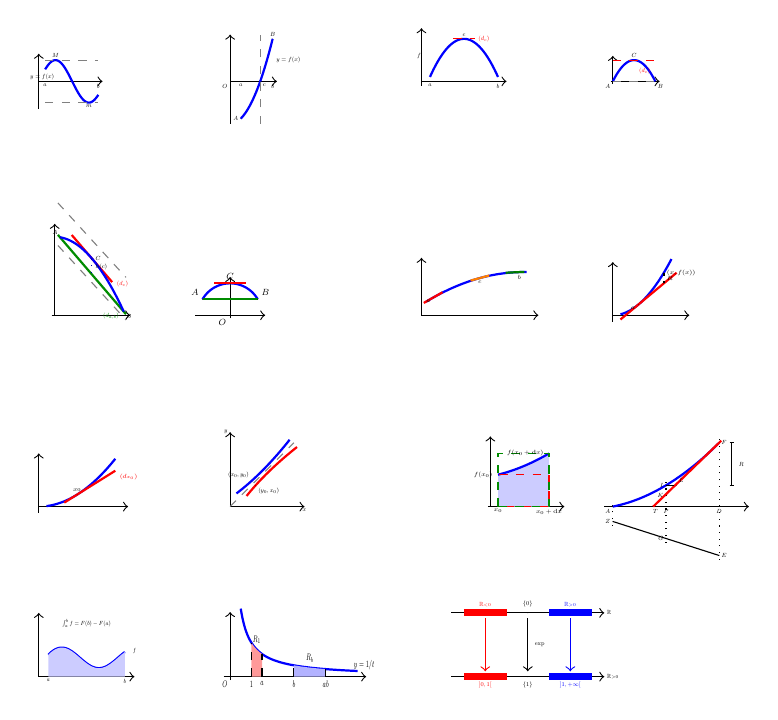
\begin{tikzpicture}[scale=0.27, transform shape, font=\footnotesize]
		
		\begin{scope}[shift={(0,0)}]
		\draw[->] (0,-1.3) -- (0,0) -- (3,0);
		\draw[->] (0,0) -- (0,1.3);
		\draw[blue,thick,domain=0.3:2.8,samples=80,smooth] plot (\x,{sin(2*\x r)});
		\draw[dashed,gray] (0.3,1) -- (2.8,1);
		\draw[dashed,gray] (0.3,-1) -- (2.8,-1);
		\fill (0.785,1) circle (0.4pt);  \node[above] at (0.785,1) {$M$};
		\fill (2.356,-1) circle (0.4pt); \node[below] at (2.356,-1) {$m$};
		\node[below] at (0.3,0) {$a$};   \node[below] at (2.8,0) {$b$};
		\node[left] at (0.85,0.2) {$y=f(x)$};
		\end{scope}
		
		\begin{scope}[shift={(9,0)}]
		\draw[->] (0,-2) -- (0,0) -- (2.2,0);
		\draw[->] (0,0) -- (0,2.2);
		\draw[blue,thick,domain=0.5:2,samples=60,smooth] plot (\x,{\x*\x-2});
		\draw[dotted] (0,0) -- (2.1,0);
		\draw[dashed,gray] (1.414,-2) -- (1.414,2.2);
		\fill (0.5,-1.75) circle (0.4pt); \node[left] at (0.5,-1.75) {$A$};
		\fill (2,2) circle (0.4pt);       \node[above] at (2,2) {$B$};
		\fill (1.414,0) circle (0.4pt);   \node[below right] at (1.414,0) {$c$};
		\node[below] at (0.5,0) {$a$};    \node[below] at (2,0) {$b$};
		\node[below left] at (0,0) {$O$};
		\node[right] at (2.05,1) {$y=f(x)$};
		\end{scope}
		
		\begin{scope}[shift={(18,0)}]
		\draw[->] (0,0) -- (4,0);
		\draw[->] (0,-0.2) -- (0,2.5);
		\draw[blue,thick,domain=0.4:3.6,samples=60,smooth] plot (\x,{2-0.7*(\x-2)*(\x-2)});
		\draw[dashed,red] (1.5,2) -- (2.5,2);
		\fill (2,2) circle (0.4pt); \node[above] at (2,2) {$c$};
		\node[below] at (0.4,0) {$a$}; \node[below] at (3.6,0) {$b$};
		\node[left] at (0.1,1.2) {$f$};
		\node[right] at (2.55,2) {\textcolor{red}{$(d_c)$}};
		\end{scope}
		
		\begin{scope}[shift={(27,0)}]
		\draw[->] (-0.1,0) -- (2.2,0); \draw[->] (0,-0.1) -- (0,1.2);
		\draw[blue,thick,domain=0:2,samples=80] plot (\x,{\x*(2-\x)});
		\draw[dashed,gray] (0,0)--(2,0); \draw[dashed,red] (0,1)--(2,1);
		\fill (0,0) circle (0.4pt); \node[below left] at (0,0) {$A$};
		\fill (2,0) circle (0.4pt); \node[below right] at (2,0) {$B$};
		\fill (1,1) circle (0.4pt); \node[above] at (1,1) {$C$};
		\node[below] at (1.5,0.75) {\textcolor{red}{$(d_c)$}};
		\end{scope}
		
		\begin{scope}[shift={(0,-11)}]
		\draw[->] (0.6,0) -- (4.3,0); \draw[->] (0.75,0) -- (0.75,4.3);
		\draw[dashed,gray] (0.9,3.283)--(4.1,-0.217); \draw[dashed,gray] (0.9,5.283)--(4.1,1.783);
		\draw[green!55!black,thick] (0.9,3.783)--(4.1,0.05);
		\draw[red,thick] (1.55,3.775)--(3.45,1.559);
		\draw[blue,thick,domain=1:4,samples=120,smooth] plot (\x,{-\x*\x/3+\x/2+3.5});
		\fill (1,3.667) circle (0.4pt); \node[above left] at (1,3.667) {$A$};
		\fill (4,0.167) circle (0.4pt); \node[below right] at (4,0.167) {$B$};
		\fill (2.5,2.667) circle (0.4pt); \node[right] at (2.55,2.667) {$C$};
		\draw[dotted,blue!70!black] (2.5,2.667) -- (2.5,1.917);
		\node[right] at (2.55,2.29) {$h(c)$};
		\node[below] at (3.4,0.25) {\textcolor{green!55!black}{$(d_{a,b})$}};
		\node[right] at (3.55,1.45) {\textcolor{red}{$(d_c)$}};
		\end{scope}
		
		\begin{scope}[shift={(9,-11)},xscale=1.5,yscale=1.5]
		\draw[->] (-1.1,0) -- (1.1,0); \draw[->] (0,-0.1) -- (0,1.2);
		\draw[blue,thick,domain=0.5236:2.618,samples=100,smooth] plot ({cos(\x r)},{sin(\x r)});
		\draw[green!55!black,thick] (-0.866,0.5)--(0.866,0.5);
		\draw[red,thick] (-0.5,1)--(0.5,1);
		\fill (-0.866,0.5) circle (0.4pt); \node[above left] at (-0.866,0.5) {$A$};
		\fill (0.866,0.5) circle (0.4pt); \node[above right] at (0.866,0.5) {$B$};
		\fill (0,1) circle (0.4pt); \node[above] at (0,1) {$C$};
		\node[below left] at (0,0) {$O$};
		\end{scope}
		
		\begin{scope}[shift={(18,-11)},xscale=1.1]
		\draw[->] (0,0) -- (5,0); \draw[->] (0,0) -- (0,2.7);
		\draw[blue,thick,domain=0.2:4.5,samples=100] plot (\x,{0.5+0.7*\x-0.08*\x*\x});
		\draw[red,thick] (0.1,0.58)--(0.9,1.08);
		\draw[orange,thick] (2.1,1.63)--(2.9,1.87);
		\draw[green!50!black,thick] (3.6,2.00)--(4.4,2.04);
		\fill (0.5,0.83) circle (0.4pt); \node[below left] at (0.5,0.83) {$a$};
		\fill (2.5,1.75) circle (0.4pt); \node[below] at (2.5,1.75) {$c$};
		\fill (4,2.02) circle (0.4pt); \node[below right] at (4,2.02) {$b$};
		\end{scope}
		
		\begin{scope}[shift={(27,-11)},xscale=1.2]
		\draw[->] (0,0) -- (3,0); \draw[->] (0,-0.3) -- (0,2.5);
		\draw[blue,thick,domain=0.3:2.3,samples=60] plot (\x,{\x*\x/2});
		\draw[red,thick] (0.3,-0.2)--(2.5,2.0);
		\fill (1,0.5) circle (0.4pt); \node[below left] at (1,0.5) {$a$};
		\fill (2,2) circle (0.4pt); \node[right] at (2,2) {$(x,f(x))$};
		\fill (2,1.5) circle (0.4pt);
		\draw[dotted,thick] (2,1.5)--(2,2);
		\node[right] at (2,1.75) {$R$};
		\end{scope}
		
		\begin{scope}[shift={(0,-20)},xscale=1.2]
		\draw[->] (0,0) -- (3.5,0); \draw[->] (0,-0.3) -- (0,2.5);
		\draw[blue,thick,domain=0.3:3,samples=60] plot (\x,{\x*\x/4});
		\draw[red,thick] (1,0.1875)--(3,1.6875);
		\fill (1.5,0.5625) circle (0.4pt); \node[above] at (1.5,0.5625) {$x_0$};
		\node[right] at (3.05,1.40) {\textcolor{red}{$(d_{x_0})$}};
		\end{scope}
		
		\begin{scope}[shift={(9,-20)}]
		\draw[->] (0,0) -- (3.5,0) node[below] {$x$};
		\draw[->] (0,0) -- (0,3.5) node[left] {$y$};
		\draw[dashed,gray] (0,0)--(3,3);
		\draw[blue,thick,domain=0.3:2.8,samples=80] plot (\x,{0.4+0.7*\x+0.1*\x*\x});
		\draw[red,thick,domain=0.5:2.8,samples=80] plot ({0.4+0.7*\x+0.1*\x*\x},{\x});
		\fill (1,1.2) circle (0.4pt); \node[above left] at (1,1.2) {$(x_0,y_0)$};
		\fill (1.2,1) circle (0.4pt); \node[below right] at (1.2,1) {$(y_0,x_0)$};
		\end{scope}
		
		\begin{scope}[shift={(18,-20)},xscale=1.2,yscale=1.0]
		\draw[->] (2.6,0) -- (5.6,0); \draw[->] (2.7,0) -- (2.7,3.3);
		\fill[blue!20] (3,0) -- plot[domain=3:5,samples=60] (\x,{1.5+0.3*(\x-3)+0.1*(\x-3)*(\x-3)}) -- (5,0) -- cycle;
		\draw[blue,thick,domain=3:5,samples=60,smooth] plot (\x,{1.5+0.3*(\x-3)+0.1*(\x-3)*(\x-3)});
		\draw[dashed,red] (3,0) rectangle (5,1.5);
		\draw[dashed,green!55!black] (3,0) rectangle (5,2.5);
		\fill (3,0) circle (0.4pt); \node[below] at (3,0) {$x_0$};
		\fill (5,0) circle (0.4pt); \node[below] at (5,0) {$x_0+\mathrm{d}x$};
		\node[left] at (2.9,1.5) {$f(x_0)$};
		\node[left] at (4.9,2.5) {$f(x_0+\mathrm{d}x)$};
		\end{scope}
		
		\begin{scope}[shift={(27,-20)}]
		\draw[->] (-0.4,0) -- (6.4,0);
		\draw[dotted] (0,-0.9) -- (0,0.3);
		\draw[dotted] (2.5,-1.7) -- (2.5,1.3);
		\draw[dotted] (5,-2.5) -- (5,3.4);
		\draw plot[smooth,tension=0.7] coordinates {(0,-0.7) (2.5,-1.5) (5,-2.3)};
		\draw[blue,thick,domain=0:5,samples=100,smooth] plot (\x,{0.08*\x*\x+0.2*\x});
		\draw[red,thick] (1.9,0)--(5.1,3.1);
		\draw[dashed] (2.5,1) -- (3,1);
		\fill (0,0) circle (0.4pt);    \node[below left]  at (0,0)    {$A$};
		\fill (2,0) circle (0.4pt);    \node[below]       at (2,0)    {$T$};
		\fill (2.5,0) circle (0.4pt);  \node[below]       at (2.5,0)  {$P$};
		\fill (5,0) circle (0.4pt);    \node[below]       at (5,0)    {$D$};
		\fill (0,-0.7) circle (0.4pt); \node[left]        at (0,-0.7) {$Z$};
		\fill (2.5,-1.5) circle (0.4pt);\node[left]       at (2.5,-1.5){$G$};
		\fill (5,-2.3) circle (0.4pt); \node[right]       at (5,-2.3) {$E$};
		\fill (2.5,1) circle (0.4pt);  \node[left]        at (2.5,1)  {$I$};
		\fill (2.5,0.5) circle (0.4pt);\node[left]        at (2.5,0.5){$K$};
		\fill (3,1) circle (0.4pt);    \node[above right] at (3,1)    {$L$};
		\fill (5,3) circle (0.4pt);    \node[right]       at (5,3)    {$F$};
		\draw (5.5,1) -- (5.7,1); \draw (5.5,3) -- (5.7,3); \draw (5.6,1) -- (5.6,3);
		\node[right] at (5.8,2) {$R$};
		\end{scope}
		
		\begin{scope}[shift={(0,-28)},xscale=0.9]
		\draw[->] (0,0) -- (5,0); \draw[->] (0,0) -- (0,3);
		\draw[blue,thick,domain=0.5:4.5,samples=80] plot (\x,{0.5+0.6*sin(\x*1.5 r)+0.5*sin(\x*0.5 r)});
		\fill[blue!20] (0.5,0) -- plot[domain=0.5:4.5,samples=80] (\x,{0.5+0.6*sin(\x*1.5 r)+0.5*sin(\x*0.5 r)}) -- (4.5,0) -- cycle;
		\node[above] at (2.5,2.2) {$\int_a^b f = F(b)-F(a)$};
		\node[below] at (0.5,0) {$a$}; \node[below] at (4.5,0) {$b$};
		\node[right] at (4.8,1.2) {$f$};
		\end{scope}
		
		\begin{scope}[shift={(9,-28)},xscale=1.0,yscale=1.6]
		\draw[->] (-0.3,0) -- (6.4,0); \draw[->] (0,-0.1) -- (0,1.9);
		\draw[blue,thick,domain=0.5:6,samples=150,smooth] plot (\x,{1/\x});
		\fill[red!40] (1,0) -- plot[domain=1:1.5,samples=30] (\x,{1/\x}) -- (1.5,0) -- cycle;
		\fill[blue!30] (3,0) -- plot[domain=3:4.5,samples=30] (\x,{1/\x}) -- (4.5,0) -- cycle;
		\draw[dashed] (1,0) -- (1,1); \draw[dashed] (1.5,0) -- (1.5,0.667);
		\draw[dashed] (3,0) -- (3,0.333); \draw[dashed] (4.5,0) -- (4.5,0.222);
		\node[below] at (1,0) {$1$}; \node[below] at (1.5,0) {$a$};
		\node[below] at (3,0) {$b$}; \node[below] at (4.5,0) {$ab$};
		\node[above] at (1.25,0.85) {$R_1$};
		\node[above] at (3.75,0.30) {$R_b$};
		\node[right] at (5.7,0.35) {$y=1/t$};
		\node[below left] at (0,0) {$O$};
		\end{scope}
		
	\begin{scope}[shift={(20,-25)}]
	\draw[->] (-0.6,0) -- (6.6,0) node[right] {$\R$};
	\draw[red,line width=2.5pt] (0,0)--(2,0);
	\draw[blue,line width=2.5pt] (4,0)--(6,0);
	\fill (3,0) circle (0.5pt);
	\node[above=4pt] at (1,0) {\textcolor{red}{$\R_{<0}$}};
	\node[above=4pt] at (3,0) {$\{0\}$};
	\node[above=4pt] at (5,0) {\textcolor{blue}{$\R_{>0}$}};
	\draw[->,red]  (1,-0.25) -- (1,-2.75);
	\draw[->]      (3,-0.25) -- (3,-2.75);
	\draw[->,blue] (5,-0.25) -- (5,-2.75);
	\node[right=6pt] at (3,-1.5) {$\exp$};
	\draw[->] (-0.6,-3) -- (6.6,-3) node[right] {$\R_{>0}$};
	\draw[red,line width=2.5pt] (0,-3)--(2,-3);
	\draw[blue,line width=2.5pt] (4,-3)--(6,-3);
	\fill (3,-3) circle (0.5pt);
	\node[below=4pt] at (1,-3) {\textcolor{red}{${]}0,1[$}};
	\node[below=4pt] at (3,-3) {$\{1\}$};
	\node[below=4pt] at (5,-3) {\textcolor{blue}{${]}1,+\infty[$}};
	\end{scope}
		\end{tikzpicture}}
\end{figure}
\newpage \thispagestyle{empty} \newpage \hypersetup{pageanchor=true} %
\pagestyle{plain}\pagenumbering{arabic}

\section*{Introduction}

\label{sec:introduction} \setstretch{1.3} \noindent Barrow's \emph{%
Geometrical Lectures} (1670) give the first calculus textbook and the first
geometric proof of the Fundamental Theorem of Calculus; see \cite%
{Barrow1916,Lopez2026}.

\autoref{part:part1} develops the classical theorems of single-variable real
analysis --- EVT,\,\allowbreak IVT,\,\allowbreak Fermat,\,\allowbreak
Rolle,\,\allowbreak MVT and its refinements,\,\allowbreak
convexity,\,\allowbreak inverse function,\,\allowbreak the Fundamental
Theorems of Calculus,\,\allowbreak and the $\ln$/$\exp$ addition and image
theorems --- in Barrow's geometric idiom,\,\allowbreak with figures and
geometric proofs.

\autoref{part:part2} classifies each theorem in reverse mathematics. Every
axiom,\,\allowbreak postulate,\,\allowbreak definition and statement of %
\autoref{part:part1} reappears as a tagged entry with a dependency table and
an exact strength. Classification: all entries are $\mathsf{RCA}_0$ except
IVT,\,\allowbreak EVT,\,\allowbreak Darboux,\,\allowbreak and the weighted
MVT,\,\allowbreak which are $\mathsf{WKL}_0$. No \autoref{part:part2} entry
uses Cauchy completeness or any form of Choice \cite{Propp2012,Jech1973}.
Coding conventions are in \S \ref{sec:coding}.

\part{A Geometric Development of Classical Real Analysis}

\label{part:part1} \noindent Following Barrow \cite[Lecture~X, \S 11]%
{Barrow1916},\,\allowbreak we state and prove the classical theorems in
Barrow's geometric idiom. See \cite{Lopez2026} for commentary.

\section{Axioms, definitions and geometric conventions}

\label{sec:conventions}

Let $[a,\,\allowbreak b]\subseteq\R$ and let $f\colon[a,\,\allowbreak b]\to%
\R
$ be continuous. The \emph{area function of $f$} is the function $A_{a,f}$
defined for $x\in[a,\,\allowbreak b]$ by 
\begin{equation}  \label{eq:area}
A_{a,f}^{x}:=\text{(signed) area of }\{(t,\,\allowbreak y): a\le t\le
x,\,\allowbreak\ 0\le y\le f(t)\},\,\allowbreak
\end{equation}
and we write $A_a^x$ for $A_{a,f}^x$ whenever the ambient function $f$ is
clear from context.

with Barrow's orientation: for all $u,\,\allowbreak w\in[a,\,\allowbreak b]$%
, 
\begin{equation}  \label{eq:oriented-area}
A_u^{u}=0,\,\allowbreak\qquad A_u^{w}=-A_w^{u},\,\allowbreak
\end{equation}
and in particular $A_x^{x+\mathrm{d}x}=-A_{x+\mathrm{d}x}^{x}$ for $\mathrm{d%
}x<0$. Equivalently, $A$ is additive over intervals: $A_u^w=A_u^v+A_v^w$ for
all $u,\,\allowbreak v,\,\allowbreak w\in[a,\,\allowbreak b]$, which is %
\autoref{eq:lin-int}. The curve $u\mapsto A_a^u$ is Barrow's $AIF$; $f(x_0)$
is his $DE$; the unit is his $R$.

\paragraph{$\mathsf{\protect\underline{Differentiability.}}$}

\text{\ } $f$ is differentiable at $x$ if 
\begin{equation}  \label{eq:diff}
\lim_{h\to 0}(f(x+h)-f(x))/h=f^{\prime }(x)
\end{equation}
exists.

\paragraph{\textsf{\protect\underline{Tangency (little-\textit{o} form).}}}

Let $G$ be defined on an open interval containing $x_0\in\R$, and let $%
L(u)=m(u-x_0)+b$ be a line ($m,\,\allowbreak b\in\R$). Then $G$ is
differentiable at $x_0$ with tangent line $L$ if and only if 
\begin{equation}  \label{eq:little-o}
L(x_0)=G(x_0)\quad\text{and}\quad G(x_0+\Delta x)=G(x_0)+m\,\Delta x+\Delta
x\cdot o(\Delta x)\quad(\Delta x\to0),\,\allowbreak
\end{equation}
in which case $G^{\prime }(x_0)=m$; cf.\ \cite[Theorem~2]{Lopez2026}.

\paragraph{$\mathsf{\protect\underline{Lin-Integ.}}$}

\text{\ } 
\begin{equation}  \label{eq:lin-int}
\forall u,\,\allowbreak v,\,\allowbreak w\in[a,\,\allowbreak b]:\
A_u^w=A_u^v+A_v^w.
\end{equation}

\paragraph{$\mathsf{\protect\underline{Int-Mono.}}$}

\text{\ } 
\begin{equation}  \label{eq:int-mono}
f\le g\ \text{on}\ [a,\,\allowbreak b]\Rightarrow\int_a^b f\le\int_a^b g.
\end{equation}

\paragraph{$\mathsf{\protect\underline{Similarity.}}$}

\text{\ } For $b>0$,\,\allowbreak 
\begin{equation}  \label{eq:similarity}
\int_b^{ab} h(t)\,\mathrm{d}t=\int_1^a h(bu)\,b\,\mathrm{d}u.
\end{equation}

\paragraph{$\mathsf{\protect\underline{Inv-Cont.}}$}

\text{\ } 
\begin{equation}  \label{eq:inv-cont}
t\mapsto1/t\in C^0(\R_{>0}).
\end{equation}

\paragraph{$\mathsf{\protect\underline{Image-Union.}}$}

\text{\ } 
\begin{equation}  \label{eq:image-union}
f(A\cup B)=f(A)\cup f(B).
\end{equation}

\paragraph{$\mathsf{\protect\underline{Product\,rule.}}$}

\text{\ } 
\begin{equation}  \label{eq:product-rule}
(fg)^{\prime }(x)=f^{\prime }(x)g(x)+f(x)g^{\prime }(x).
\end{equation}

\paragraph{$\mathsf{\protect\underline{Chain\,rule.}}$}

\text{\ } 
\begin{equation}  \label{eq:chain-rule}
(f\circ g)^{\prime }(x)=f^{\prime }(g(x))\,g^{\prime }(x).
\end{equation}

\paragraph{$\mathsf{\protect\underline{Logarithm.}}$}

\text{\ } For $x>0$,\,\allowbreak set 
\begin{equation}  \label{eq:def-ln}
\ln(x):=\int_1^x \frac{\mathrm{d}t}{t}.
\end{equation}
By \autoref{eq:inv-cont} the integrand $t\mapsto 1/t$ is continuous on $\R%
_{>0}$,\,\allowbreak so the integral is well defined.

\paragraph{$\mathsf{\protect\underline{Sign-Law.}}$}

\text{\ } 
\begin{equation}  \label{eq:sign-law}
\forall u>0:\ \bigl(\ln u<0\iff u<1\bigr)\wedge\bigl(\ln u=0\iff u=1\bigr)%
\wedge\bigl(\ln u>0\iff u>1\bigr).
\end{equation}

\paragraph{$\mathsf{\protect\underline{Ln-Bij.}}$}

\text{\ } The map $\ln:\R_{>0}\to\R$ of \autoref{eq:def-ln} is bijective;
the \emph{exponential} is defined as its inverse: 
\begin{equation}  \label{eq:ln-bij}
\ln:\R_{>0}\to\R\ \text{bijective},\,\allowbreak\qquad \exp:=\ln^{-1}\colon\R%
\to\R_{>0}.
\end{equation}
Equivalently, $\ln(\exp u)=u$ for all $u\in\R$ and $\exp(\ln a)=a$ for all $%
a>0$.

\paragraph{$\mathsf{\protect\underline{Barrow-tangency.}}$}

\text{\ } Let $G$ be differentiable at $x_0$,\,\allowbreak and let $%
L(u)=m(u-x_0)+G(x_0)$ be the line through $(x_0,\,\allowbreak G(x_0))$ of
slope $m$. If $L\le G$ (or $L\ge G$) on a punctured neighbourhood of $x_0$%
,\,\allowbreak then\footnote{%
The two-sided hypothesis strengthens Barrow's one-sided
criterion,\,\allowbreak which fails at inflections \cite{Lopez2026}. Every
use in \autoref{part:part1} is in a convex or concave setting,\,\allowbreak
where the two-sided hypothesis holds.} 
\begin{equation}  \label{eq:barrow-tangency}
m=G^{\prime }(x_0).
\end{equation}

\section{Statements of the classical theorems}

\subsection{Topological theorems}

\begin{theorem}[Extreme Value Theorem]
\label{thm:evt} If $f:[a,\,\allowbreak b]\to\R$ is continuous,\,\allowbreak
then 
\begin{equation}  \label{eq:evt}
\exists x_{\max},\,\allowbreak x_{\min}\in[a,\,\allowbreak b],\,\allowbreak\
\forall x\in[a,\,\allowbreak b]:\ f(x_{\min})\le f(x)\le f(x_{\max}).
\end{equation}
\end{theorem}

\begin{theorem}[Intermediate Value Theorem]
\label{thm:ivt} If $f:[a,\,\allowbreak b]\to\R$ is continuous and $f(a)f(b)<0
$,\,\allowbreak then 
\begin{equation}  \label{eq:ivt}
\exists c\in(a,\,\allowbreak b):\ f(c)=0.
\end{equation}
\end{theorem}

\subsection{Differentiation theorems}

\paragraph{$\mathsf{\protect\underline{Chord and tangent lines.}}$}

\text{\ } For $f:[a,\,\allowbreak b]\to\R$ and distinct $u,\,\allowbreak v\in%
[a,\,\allowbreak b]$, the \emph{chord line of $f$ through $u$ and $v$} is
the unique affine line through the points $(u,\,\allowbreak f(u))$ and $%
(v,\,\allowbreak f(v))$; in coordinates, 
\begin{equation}  \label{eq:chord-line}
d_{u,v}:=\Bigl\{(x,\,\allowbreak y)\in\R^{2}:\ y=\frac{f(v)-f(u)}{v-u}%
\,(x-u)+f(u)\Bigr\}.
\end{equation}
For $x_0\in(a,\,\allowbreak b)$ at which $f$ is differentiable, the \emph{%
tangent line to $f$ at $x_0$} is 
\begin{equation}  \label{eq:tangent-line}
d_{x_0}:=\bigl\{(x,\,\allowbreak y)\in\R^{2}:\ y=f^{\prime
}(x_0)\,(x-x_0)+f(x_0)\bigr\}.
\end{equation}
Two such lines are \emph{parallel}, written $(d_1)\parallel (d_2)$, iff they
have the same slope; in particular, $(d_c)\parallel (d_{a,b})$ iff $%
f^{\prime }(c)=\dfrac{f(b)-f(a)}{b-a}$.

\begin{theorem}[Fermat]
\label{thm:fermat} If $f$ has a local extremum at $c\in(a,\,\allowbreak b)$
and is differentiable at $c$,\,\allowbreak then 
\begin{equation}  \label{eq:fermat}
f^{\prime }(c)=0.
\end{equation}
\end{theorem}

\begin{theorem}[Rolle]
\label{thm:rolle} If $f$ is continuous on $[a,\,\allowbreak b]$%
,\,\allowbreak differentiable on $(a,\,\allowbreak b)$,\,\allowbreak and $%
f(a)=f(b)$,\,\allowbreak then 
\begin{equation}
\exists c\in(a,\,\allowbreak b):\,f^{\prime }(c)=0.
\end{equation}
\end{theorem}

\begin{theorem}[Mean-Value Theorem]
\label{thm:mvt} If $f$ is continuous on $[a,\,\allowbreak b]$ and
differentiable on $(a,\,\allowbreak b)$,\,\allowbreak then 
\begin{equation}  \label{eq:mvt}
\exists c\in(a,\,\allowbreak b):\ f^{\prime }(c)=\frac{f(b)-f(a)}{b-a}.
\end{equation}
Geometrically,\,\allowbreak $(d_c)\parallel (d_{a,\,\allowbreak b})$.
\end{theorem}

\begin{theorem}[Constant-function]
\label{thm:const} If $f$ is continuous on $[a,\,\allowbreak b]$%
,\,\allowbreak differentiable on $(a,\,\allowbreak b)$,\,\allowbreak and $%
f^{\prime }=0$ on $(a,\,\allowbreak b)$,\,\allowbreak then 
\begin{equation}  \label{eq:const}
f(x)=f(a)\quad\text{for all }x\in[a,\,\allowbreak b].
\end{equation}
\end{theorem}

\begin{theorem}[Monotonicity]
\label{thm:monotone} If $f$ is continuous on $[a,\,\allowbreak b]$%
,\,\allowbreak differentiable on $(a,\,\allowbreak b)$,\,\allowbreak and $%
f^{\prime }\ge0$ (resp.\ $f^{\prime }>0$),\,\allowbreak then 
\begin{equation}  \label{eq:monotone}
x<y\Rightarrow f(x)\le f(y)\quad\text{(resp.\ }f(x)<f(y)\text{)}
\end{equation}
for all $x,\,\allowbreak y\in[a,\,\allowbreak b]$.
\end{theorem}

\begin{theorem}[Cauchy MVT]
\label{thm:cauchy-mvt} If $f,\,\allowbreak g$ are continuous on $%
[a,\,\allowbreak b]$,\,\allowbreak differentiable on $(a,\,\allowbreak b)$%
,\,\allowbreak and $g^{\prime }\ne0$ on $(a,\,\allowbreak b)$,\,\allowbreak
then 
\begin{equation}  \label{eq:cauchy-mvt}
\exists c\in(a,\,\allowbreak b):\ \frac{f^{\prime }(c)}{g^{\prime }(c)}=%
\frac{f(b)-f(a)}{g(b)-g(a)}.
\end{equation}
\end{theorem}

\begin{theorem}[Darboux]
\label{thm:darboux} If $f$ is differentiable on $[a,\,\allowbreak b]$ and $%
f^{\prime }(a)<\lambda<f^{\prime }(b)$,\,\allowbreak then 
\begin{equation}  \label{eq:darboux}
\exists c\in(a,\,\allowbreak b):\ f^{\prime }(c)=\lambda.
\end{equation}
\end{theorem}

\begin{theorem}[L'H\^opital]
\label{thm:lhopital} Let $f,\,\allowbreak g$ be differentiable near $a$%
,\,\allowbreak with $f(a)=g(a)=0$,\,\allowbreak $g^{\prime }\ne0$ near $a$%
,\,\allowbreak and 
\begin{equation*}
\lim_{x\to a}f^{\prime }(x)/g^{\prime }(x)=L.
\end{equation*}
Then 
\begin{equation}  \label{eq:lhopital}
\lim_{x\to a}f(x)/g(x)=L.
\end{equation}
\end{theorem}

\begin{theorem}[Taylor,\,\allowbreak Lagrange remainder]
\label{thm:taylor} If $f$ is $(n+1)$-times differentiable on an interval
containing $a$ and $x$,\,\allowbreak then 
\begin{equation}  \label{eq:taylor}
\exists c\ \text{between}\ a,\,\allowbreak x:\ f(x)=\sum_{k=0}^{n}\frac{%
f^{(k)}(a)}{k!}(x-a)^{k}+\frac{f^{(n+1)}(c)}{(n+1)!}(x-a)^{n+1}.
\end{equation}
\end{theorem}

\begin{theorem}[Convexity]
\label{thm:convexity} If $f$ is twice differentiable on $[a,\,\allowbreak b] 
$ and $f^{\prime \prime }\ge0$ on $(a,\,\allowbreak b)$,\,\allowbreak then 
\begin{equation}  \label{eq:convexity}
f(x)\ge f(x_0)+f^{\prime }(x_0)(x-x_0)\quad\text{for all }x,\,\allowbreak x_0%
\in[a,\,\allowbreak b].
\end{equation}
\end{theorem}

\begin{theorem}[Inverse function]
\label{thm:inverse} If $f:I\to\R$ is continuous and strictly monotone on $I$%
,\,\allowbreak $x_0$ lies in the interior $I^\circ$ of $I$,\,\allowbreak and 
$f$ is differentiable at $x_0$ with $f^{\prime }(x_0)\ne0$,\,\allowbreak
then $f^{-1}$ is differentiable at $y_0=f(x_0)$ with 
\begin{equation}  \label{eq:inverse}
(f^{-1})^{\prime }(y_0)=1/f^{\prime }(x_0).
\end{equation}
\end{theorem}

\subsection{Integration theorems}

\begin{lemma}[Barrow's area inequality]
\label{lem:barrow-area} If $f$ is continuous and increasing on $%
[a,\,\allowbreak b]$ and $x_0,\,\allowbreak x_0+\mathrm{d}x\in[%
a,\,\allowbreak b]$,\,\allowbreak $\mathrm{d}x\ne0$,\,\allowbreak then 
\begin{equation}  \label{eq:barrow-area}
f(x_0)\,\mathrm{d}x\le A_{x_0}^{x_0+\mathrm{d}x}\le f(x_0+\mathrm{d}x)\,%
\mathrm{d}x,
\end{equation}
and both inequalities are strict when $f$ is strictly increasing on the
interval with endpoints $x_0$ and $x_0+\mathrm{d}x$.
\end{lemma}

\begin{lemma}[MVT for integrals]
\label{lem:mvt-int} If $f$ is continuous on $[a,\,\allowbreak b]$ and $%
x_0,\,\allowbreak x_0+\mathrm{d}x\in[a,\,\allowbreak b]$,\,\allowbreak $%
\mathrm{d}x\ne0$,\,\allowbreak then 
\begin{equation}  \label{eq:mvt-int}
\exists\theta\ \text{between}\ x_0,\,\allowbreak x_0+\mathrm{d}x:\
A_{x_0}^{x_0+\mathrm{d}x}=f(\theta)\,\mathrm{d}x.
\end{equation}
\end{lemma}

\begin{theorem}[First FTC; Barrow]
\label{thm:fftc} If $f$ is continuous on $[a,\,\allowbreak b]$,\,\allowbreak
then 
\begin{equation}  \label{eq:fftc}
\frac{d}{dx}\int_a^x f=f(x)
\end{equation}
for every $x\in(a,\,\allowbreak b)$,\,\allowbreak with one-sided versions at 
$a,\,\allowbreak b$.
\end{theorem}

\begin{theorem}[Second FTC]
\label{thm:second-ftc} If $F$ is differentiable on $[a,\,\allowbreak b]$ and 
$F^{\prime }=f$ is continuous,\,\allowbreak then 
\begin{equation}  \label{eq:second-ftc}
\int_a^b f=F(b)-F(a).
\end{equation}
\end{theorem}

\begin{theorem}[Integration by parts]
\label{thm:ibp} If $f,\,\allowbreak g\in C^1([a,\,\allowbreak b])$%
,\,\allowbreak then 
\begin{equation}  \label{eq:ibp}
\int_a^b fg^{\prime }=[fg]_a^b-\int_a^b f^{\prime }g.
\end{equation}
\end{theorem}

\begin{theorem}[Change of variables]
\label{thm:subst} If $g\in C^1([a,\,\allowbreak b])$ and $f$ is continuous
on $g([a,\,\allowbreak b])$,\,\allowbreak then 
\begin{equation}  \label{eq:subst}
\int_{g(a)}^{g(b)}f=\int_a^b f(g)\,g^{\prime }.
\end{equation}
\end{theorem}

\begin{theorem}[Weighted MVT]
\label{thm:weighted-mvt} If $f$ is continuous on $[a,\,\allowbreak b]$%
,\,\allowbreak $w\ge0$ is Riemann integrable,\,\allowbreak and $\int_a^b w>0$%
,\,\allowbreak then 
\begin{equation}  \label{eq:weighted-mvt}
\exists c\in[a,\,\allowbreak b]:\ \int_a^b fw=f(c)\int_a^b w.
\end{equation}
\end{theorem}

\subsection{The logarithm and the exponential}

\begin{theorem}[Log\,-Property]
\label{thm:log} With $\ln(x):=\int_1^x \mathrm{d}t/t$ ($x>0$),\,\allowbreak 
\begin{equation}  \label{eq:log}
\forall a,\,\allowbreak b>0:\ \ln(a)+\ln(b)=\ln(ab).
\end{equation}
\end{theorem}

\begin{theorem}[Exp\,-Property]
\label{thm:exp} With $\exp:=\ln^{-1}$,\,\allowbreak 
\begin{equation}  \label{eq:exp}
\forall u,\,\allowbreak v\in\R:\ \exp(u)\exp(v)=\exp(u+v).
\end{equation}
\end{theorem}

\begin{theorem}[Exp\,-Image]
\label{thm:image} 
\begin{equation}  \label{eq:image}
\exp(\R)=\R_{>0},\,\allowbreak\qquad \ln(\R_{>0})=\R.
\end{equation}
\end{theorem}

\section{Geometrical proofs}

\subsection{Topological theorems}

\begin{proof}[Proof of \autoref{thm:evt}]
Set $S=f([a,b])$; $S$ is nonempty and bounded. Let 
\begin{equation*}
M=\sup S,\qquad m=\inf S.
\end{equation*}
Were $M$ unattained, the function $1/(M-f)$ would be continuous and
unbounded on $[a,b]$, a contradiction. Hence 
\begin{equation*}
M=f(x_{\max})
\end{equation*}
for some $x_{\max}\in[a,b]$; symmetrically $m=f(x_{\min})$. Combining, 
\begin{equation*}
f(x_{\min})\le f(x)\le f(x_{\max})\qquad(x\in[a,b]),
\end{equation*}
which is \autoref{eq:evt}.\hfill$\square$
\end{proof}

\begin{figure}[]
\centering
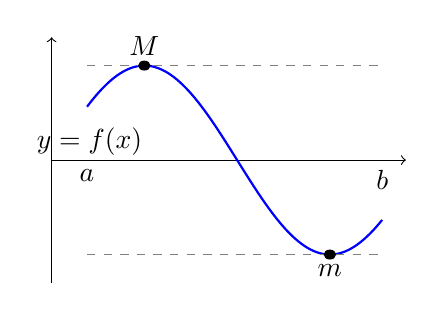
\begin{tikzpicture}[xscale=1.5,yscale=1.2]
	\draw[->] (0,-1.3) -- (0,0) -- (3,0); \draw[->] (0,0) -- (0,1.3);
	\draw[blue,thick,domain=0.3:2.8,samples=100,smooth] plot (\x,{sin(2*\x r)});
	\draw[dashed,gray] (0.3,1)--(2.8,1); \draw[dashed,gray] (0.3,-1)--(2.8,-1);
	\fill (0.785,1) circle (1.5pt); \node[above] at (0.785,1) {$M$};
	\fill (2.356,-1) circle (1.5pt); \node[below] at (2.356,-1) {$m$};
	\node[below] at (0.3,0) {$a$}; \node[below] at (2.8,0) {$b$};
	\node[left] at (0.85,0.2) {$y=f(x)$};
	\end{tikzpicture}
\caption{EVT.}
\label{fig:evt}
\end{figure}

\begin{proof}[Proof of \autoref{thm:ivt}]
Assume $f(a)<0<f(b)$ and set 
\begin{equation*}
c=\sup\{x\in[a,b]:f(x)<0\}.
\end{equation*}
By continuity, $f(c)\le 0$. If $f(c)<0$, then $f<0$ on a neighbourhood of $c$
intersected with $[a,b]$, contradicting the definition of $c$ as an upper
bound. Hence 
\begin{equation*}
f(c)=0,
\end{equation*}
which is \autoref{eq:ivt}.\hfill$\square$
\end{proof}

\begin{figure}[]
\centering
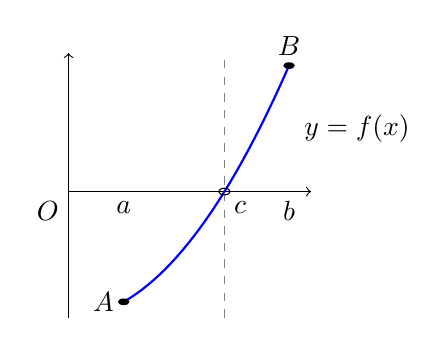
\begin{tikzpicture}[xscale=1.4,yscale=0.8]
	\draw[->] (0,-2) -- (0,0) -- (2.2,0); \draw[->] (0,0) -- (0,2.2);
	\draw[blue,thick,domain=0.5:2,samples=80,smooth] plot (\x,{\x*\x-2});
	\draw[dotted] (0,0)--(2.1,0); \draw[dashed,gray] (1.414,-2)--(1.414,2.2);
	\fill (0.5,-1.75) circle (1.5pt); \node[left] at (0.5,-1.75) {$A$};
	\fill (2,2) circle (1.5pt); \node[above] at (2,2) {$B$};
	\draw (1.414,0) circle (1.5pt); \node[below right] at (1.414,0) {$c$};
	\node[below] at (0.5,0) {$a$}; \node[below] at (2,0) {$b$};
	\node[below left] at (0,0) {$O$};
	\node[right] at (2.05,1) {$y=f(x)$};
	\end{tikzpicture}
\caption{IVT.}
\label{fig:ivt}
\end{figure}

\begin{proof}[Proof of \autoref{thm:fermat}]
Assume $c$ is a local maximum; the local-minimum case is symmetric. For $%
h>0^{+}$ small, 
\begin{equation*}
\frac{f(c+h)-f(c)}{h}\le 0 \quad\Longrightarrow\quad f^{\prime }(c)\le 0;
\end{equation*}
for $h<0^{-}$ small, 
\begin{equation*}
\frac{f(c+h)-f(c)}{h}\ge 0 \quad\Longrightarrow\quad f^{\prime }(c)\ge 0.
\end{equation*}
Hence 
\begin{equation*}
f^{\prime }(c)=0.
\end{equation*}
\hfill$\square$
\end{proof}

\begin{figure}[]
\centering
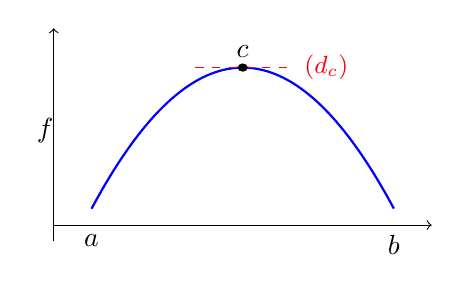
\begin{tikzpicture}[xscale=1.2]
	\draw[->] (0,0) -- (4,0); \draw[->] (0,-0.2) -- (0,2.5);
	\draw[blue,thick,domain=0.4:3.6,samples=80] plot (\x,{2-0.7*(\x-2)*(\x-2)});
	\draw[dashed,red] (1.5,2)--(2.5,2); \fill (2,2) circle (1.5pt); \node[above] at (2,2) {$c$};
	\node[below] at (0.4,0) {$a$}; \node[below] at (3.6,0) {$b$};
	\node[left] at (0.1,1.2) {$f$};
	\node[right] at (2.55,2) {\textcolor{red}{\small $(d_c)$}};
	\end{tikzpicture}
\caption{Fermat.}
\label{fig:fermat}
\end{figure}

\begin{proof}[Proof of \autoref{thm:rolle}]
By EVT, $f$ attains $M=\max_{[a,b]} f$ and $m=\min_{[a,b]} f$. If $M=m$,
then $f$ is constant and 
\begin{equation*}
f^{\prime }(c)=0\qquad(c\in(a,b)).
\end{equation*}
Otherwise $f(a)=f(b)$ forces an interior extremum $c\in(a,b)$, and Fermat's
theorem gives 
\begin{equation*}
f^{\prime }(c)=0.
\end{equation*}
\hfill$\square$
\end{proof}

\begin{figure}[]
\centering
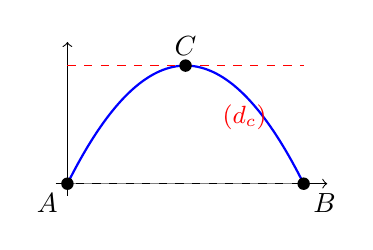
\begin{tikzpicture}[xscale=1.5,yscale=1.5]
	\draw[->] (-0.1,0) -- (2.2,0); \draw[->] (0,-0.1) -- (0,1.2);
	\draw[blue,thick,domain=0:2,samples=80] plot (\x,{\x*(2-\x)});
	\draw[dashed,gray] (0,0)--(2,0); \draw[dashed,red] (0,1)--(2,1);
	\fill (0,0) circle (1.5pt); \node[below left] at (0,0) {$A$};
	\fill (2,0) circle (1.5pt); \node[below right] at (2,0) {$B$};
	\fill (1,1) circle (1.5pt); \node[above] at (1,1) {$C$};
	\node[below] at (1.5,0.75) {\textcolor{red}{\small $(d_c)$}};
	\end{tikzpicture}
\caption{Rolle.}
\label{fig:rolle}
\end{figure}

\begin{proof}[Proof of \autoref{thm:mvt} (Barrow's sliding tangent)]
Let $L$ be the affine function whose graph is the chord line $(d_{a,b})$ of %
\autoref{eq:chord-line}, so that $L^{\prime }\equiv(f(b)-f(a))/(b-a)$; set $%
g:=f-L$. Then $g(a)=g(b)=0$. By EVT, $g$ attains $M=\max g$ and $m=\min g$. 
\emph{Case $M>0$:} the maximum is attained at some $c\in(a,b)$; the
translate $L+M$ touches $f$ at $C$ and lies above, so by concave
Barrow-tangency, 
\begin{equation*}
f^{\prime }(c)=L^{\prime }(c)=\frac{f(b)-f(a)}{b-a}.
\end{equation*}
\emph{Case $M=0$:} if $f\equiv L$ the result is trivial; otherwise $m<0$
with minimum at interior $c$, and the same argument via convex
Barrow-tangency yields 
\begin{equation*}
f^{\prime }(c)=\frac{f(b)-f(a)}{b-a}.
\end{equation*}
In either case, $(d_c)\parallel (d_{a,b})$.\hfill$\square$
\end{proof}

\begin{figure}[]
\centering
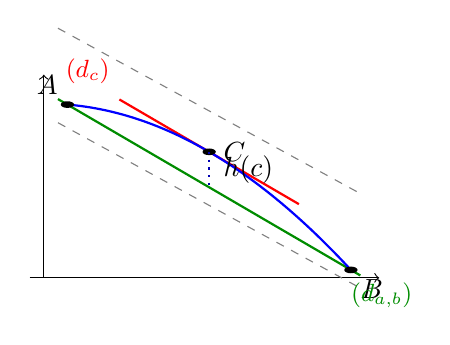
\begin{tikzpicture}[xscale=1.2,yscale=0.6]
	\draw[->] (0.6,0) -- (4.3,0); \draw[->] (0.75,0) -- (0.75,4.3);
	\draw[dashed,gray] (0.9,3.283)--(4.1,-0.217); \draw[dashed,gray] (0.9,5.283)--(4.1,1.783);
	\draw[green!55!black,thick] (0.9,3.783)--(4.1,0.05);
	\draw[red,thick] (1.55,3.775)--(3.45,1.559);
	\draw[blue,thick,domain=1:4,samples=120,smooth] plot (\x,{-\x*\x/3+\x/2+3.5});
	\fill (1,3.667) circle (2pt); \node[above left] at (1,3.667) {$A$};
	\fill (4,0.167) circle (2pt); \node[below right] at (4,0.167) {$B$};
	\fill (2.5,2.667) circle (2pt); \node[right] at (2.55,2.667) {$C$};
	\draw[dotted,blue!70!black,thick] (2.5,2.667) -- (2.5,1.917);
	\node[right] at (2.55,2.29) {$h(c)$};
	\node[below right] at (3.9,0.10) {\textcolor{green!55!black}{\small $(d_{a,b})$}};
	\node[above left] at (1.55,3.90) {\textcolor{red}{\small $(d_c)$}};
	\end{tikzpicture}
\caption{MVT sliding tangent: chord $(d_{a,b})$ (green) and tangent $(d_c)$
(red), with $(d_c)\parallel (d_{a,b})$.}
\label{fig:mvt}
\end{figure}

\begin{proof}[Proof of \autoref{thm:const}]
Apply MVT on $[a,x]$ with $x\in(a,b]$: 
\begin{equation*}
f(x)-f(a)=f^{\prime }(c)(x-a)=0.
\end{equation*}
Hence 
\begin{equation*}
f(x)=f(a)\qquad(x\in[a,b]).
\end{equation*}
\hfill$\square$
\end{proof}

\begin{proof}[Proof of \autoref{thm:monotone}]
Let $x_1<x_2$ in $[a,b]$. By MVT on $[x_1,x_2]$, there is $c\in(x_1,x_2)$
with 
\begin{equation*}
f(x_2)-f(x_1)=f^{\prime }(c)(x_2-x_1).
\end{equation*}
If $f^{\prime }\ge 0$, the right-hand side is $\ge 0$, hence $f(x_2)\ge
f(x_1)$; if $f^{\prime }>0$, it is $>0$, hence $f(x_2)>f(x_1)$.\hfill$%
\square $
\end{proof}

\begin{proof}[Proof of \autoref{thm:cauchy-mvt}]
Define 
\begin{equation*}
h:=(f(b)-f(a))\,g-(g(b)-g(a))\,f.
\end{equation*}
Then $h(a)=h(b)$, so Rolle's theorem gives $c\in(a,b)$ with 
\begin{equation*}
(f(b)-f(a))\,g^{\prime }(c)=(g(b)-g(a))\,f^{\prime }(c).
\end{equation*}
Since $g^{\prime }$ is nonzero on $(a,b)$ and $g(b)\ne g(a)$, dividing
yields 
\begin{equation*}
\frac{f^{\prime }(c)}{g^{\prime }(c)}=\frac{f(b)-f(a)}{g(b)-g(a)}.
\end{equation*}
\hfill$\square$
\end{proof}

\begin{figure}[]
\centering
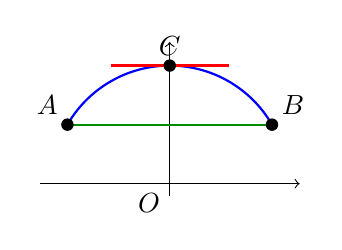
\begin{tikzpicture}[xscale=1.5,yscale=1.5]
	\draw[->] (-1.1,0) -- (1.1,0); \draw[->] (0,-0.1) -- (0,1.2);
	\draw[blue,thick,domain=0.5236:2.618,samples=100,smooth] plot ({cos(\x r)},{sin(\x r)});
	\draw[green!55!black,thick] (-0.866,0.5)--(0.866,0.5);
	\draw[red,thick] (-0.5,1)--(0.5,1);
	\fill (-0.866,0.5) circle (1.5pt); \node[above left] at (-0.866,0.5) {$A$};
	\fill (0.866,0.5) circle (1.5pt); \node[above right] at (0.866,0.5) {$B$};
	\fill (0,1) circle (1.5pt); \node[above] at (0,1) {$C$};
	\node[below left] at (0,0) {$O$};
	\end{tikzpicture}
\caption{Cauchy MVT.}
\label{fig:cauchy-mvt}
\end{figure}

\begin{proof}[Proof of \autoref{thm:darboux}]
Set $g:=f-\lambda x$; then 
\begin{equation*}
g^{\prime }(a)=f^{\prime }(a)-\lambda<0,\qquad g^{\prime }(b)=f^{\prime
}(b)-\lambda>0.
\end{equation*}
For small $h>0$, 
\begin{equation*}
g(a+h)<g(a),\qquad g(b-h)<g(b).
\end{equation*}
By EVT, $g$ attains its minimum at some $c\in[a,b]$; the above inequalities
exclude $c=a$ and $c=b$, so $c\in(a,b)$. By Fermat's theorem, 
\begin{equation*}
g^{\prime }(c)=0,\qquad\text{i.e.}\qquad f^{\prime }(c)=\lambda.
\end{equation*}
\hfill$\square$
\end{proof}

\begin{figure}[]
\centering
\begin{tikzpicture}[xscale=1.1]
	\draw[->] (0,0) -- (5,0); \draw[->] (0,0) -- (0,2.7);
	\draw[blue,thick,domain=0.2:4.5,samples=100] plot (\x,{0.5+0.7*\x-0.08*\x*\x});
	\draw[red,thick] (0.1,0.58)--(0.9,1.08);
	\draw[orange,thick] (2.1,1.63)--(2.9,1.87);
	\draw[green!50!black,thick] (3.6,2.00)--(4.4,2.04);
	\fill (0.5,0.83) circle (1.5pt); \node[below left] at (0.5,0.83) {$a$};
	\fill (2.5,1.75) circle (1.5pt); \node[below] at (2.5,1.75) {$c$};
	\fill (4,2.02) circle (1.5pt); \node[below right] at (4,2.02) {$b$};
	\end{tikzpicture}
\caption{Darboux.}
\label{fig:darboux}
\end{figure}

\begin{proof}[Proof of \autoref{thm:lhopital}]
By Cauchy MVT on $[a,x]$ with $x>a$, 
\begin{equation*}
\frac{f(x)}{g(x)}=\frac{f^{\prime }(c_x)}{g^{\prime }(c_x)},\qquad
c_x\in(a,x).
\end{equation*}
Since $c_x\to a$ as $x\to a^{+}$, 
\begin{equation*}
\lim_{x\to a^{+}}\frac{f(x)}{g(x)} =\lim_{x\to a^{+}}\frac{f^{\prime }(c_x)}{%
g^{\prime }(c_x)} =L.
\end{equation*}
The case $x\to a^{-}$ is symmetric, so the two-sided limit is $L$.\hfill$%
\square$
\end{proof}

\begin{proof}[Proof of \autoref{thm:taylor}]
Let 
\begin{equation*}
P(t):=\sum_{k=0}^{n}\frac{f^{(k)}(a)}{k!}\,(t-a)^{k}, \qquad M:=\frac{%
f(x)-P(x)}{(x-a)^{n+1}},
\end{equation*}
and define $h(t):=f(t)-P(t)-M(t-a)^{n+1}$. Then 
\begin{equation*}
h^{(j)}(a)=0\quad(j=0,\dots,n), \qquad h(x)=0.
\end{equation*}
Applying Rolle's theorem $n+1$ times gives $c$ strictly between $a$ and $x$
with 
\begin{equation*}
h^{(n+1)}(c)=0.
\end{equation*}
Since $h^{(n+1)}(t)=f^{(n+1)}(t)-M\,(n+1)!$, this yields 
\begin{equation*}
M=\frac{f^{(n+1)}(c)}{(n+1)!},
\end{equation*}
hence 
\begin{equation*}
f(x)=\sum_{k=0}^{n}\frac{f^{(k)}(a)}{k!}\,(x-a)^{k} +\frac{f^{(n+1)}(c)}{%
(n+1)!}\,(x-a)^{n+1}.
\end{equation*}
\hfill$\square$
\end{proof}

\begin{figure}[]
\centering
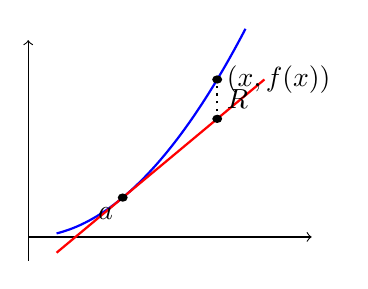
\begin{tikzpicture}[xscale=1.2]
	\draw[->] (0,0) -- (3,0); \draw[->] (0,-0.3) -- (0,2.5);
	\draw[blue,thick,domain=0.3:2.3,samples=60] plot (\x,{\x*\x/2});
	\draw[red,thick] (0.3,-0.2)--(2.5,2.0);
	\fill (1,0.5) circle (1.5pt); \node[below left] at (1,0.5) {$a$};
	\fill (2,2) circle (1.5pt); \node[right] at (2,2) {$(x,f(x))$};
	\fill (2,1.5) circle (1.5pt);
	\draw[dotted,thick] (2,1.5)--(2,2);
	\node[right] at (2,1.75) {$R$};
	\end{tikzpicture}
\caption{Taylor ($n=1$).}
\label{fig:taylor}
\end{figure}

\begin{proof}[Proof of \autoref{thm:convexity}]
Set $g(x):=f(x)-f(x_0)-f^{\prime }(x_0)(x-x_0)$. Then 
\begin{equation*}
g^{\prime \prime }=f^{\prime \prime }\ge 0,\qquad g^{\prime }(x_0)=0,\qquad
g(x_0)=0.
\end{equation*}
Since $g^{\prime }$ is nondecreasing and $g^{\prime }(x_0)=0$, we have $%
g^{\prime }(x)\le 0$ for $x<x_0$ and $g^{\prime }(x)\ge 0$ for $x>x_0$. By
the monotonicity criterion, $g$ is nonincreasing on $[a,x_0]$ and
nondecreasing on $[x_0,b]$. With $g(x_0)=0$, 
\begin{equation*}
g(x)\ge 0\qquad(x\in[a,b]),
\end{equation*}
i.e. 
\begin{equation*}
f(x)\ge f(x_0)+f^{\prime }(x_0)(x-x_0).
\end{equation*}
\hfill$\square$
\end{proof}

\begin{figure}[]
\centering
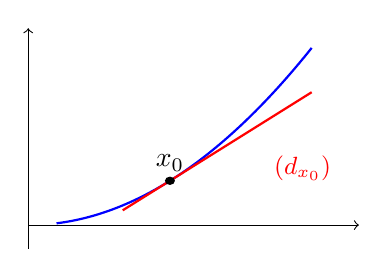
\begin{tikzpicture}[xscale=1.2]
	\draw[->] (0,0) -- (3.5,0); \draw[->] (0,-0.3) -- (0,2.5);
	\draw[blue,thick,domain=0.3:3,samples=60] plot (\x,{\x*\x/4});
\draw[red,thick] (1,0.1875)--(3,1.6875);
\fill (1.5,0.5625) circle (1.5pt); \node[above] at (1.5,0.5625) {$x_0$};
\node[below right] at (2.5,1.0) {\textcolor{red}{\small $(d_{x_0})$}};
	\end{tikzpicture}
\caption{Convexity.}
\label{fig:convexity}
\end{figure}

\begin{proof}[Proof of \autoref{thm:inverse}]
Let $c:=f^{\prime }(x_0)\ne 0$. Since $x_0\in I^\circ$, choose $\rho>0$ with 
$(x_0-\rho,x_0+\rho)\subseteq I$.

\emph{Local surjectivity.} Assume w.l.o.g.\ that $f$ is strictly increasing
on $I$ (the strictly decreasing case is symmetric). Choose $%
x_0^{-},x_0^{+}\in(x_0-\rho,x_0+\rho)$ with $x_0^{-}<x_0<x_0^{+}$. Then 
\begin{equation*}
f(x_0^{-})<y_0<f(x_0^{+}).
\end{equation*}
By IVT on the closed subinterval $[x_0^{-},x_0^{+}]\subseteq I$, every $%
y\in(f(x_0^{-}),f(x_0^{+}))$ is attained at some $x\in(x_0^{-},x_0^{+})%
\subseteq I$. Hence $(f(x_0^{-}),f(x_0^{+}))\subseteq f(I)$ is an open
neighbourhood of $y_0$, and $f^{-1}$ is defined on it.

\underline{\emph{Continuity of $f^{-1}$ at $y_0$:}}\newline
Differentiability of $f$ at $x_0$ gives $\delta_0\in(0,\rho)$ such that for
all $x$ with $|x-x_0|<\delta_0$, 
\begin{equation*}
|f(x)-f(x_0)-c(x-x_0)|<\tfrac{|c|}{2}\,|x-x_0|,
\end{equation*}
whence by the reverse triangle inequality 
\begin{equation*}
|f(x)-f(x_0)|\ge\tfrac{|c|}{2}\,|x-x_0|.
\end{equation*}
Given $\varepsilon>0$, set $\varepsilon^{\prime
}:=\min(\varepsilon,\delta_0) $ and 
\begin{equation*}
\eta:=\min\Bigl(\tfrac{|c|}{2}\,\varepsilon^{\prime },\; y_0-f(x_0^{-}),\;
f(x_0^{+})-y_0\Bigr)>0.
\end{equation*}
Suppose $|y-y_0|<\eta$.\newline
Since $y\in(f(x_0^{-}),f(x_0^{+}))\subseteq f(I)$, the value $%
x:=f^{-1}(y)\in(x_0-\rho,x_0+\rho)\subseteq I$ is defined. In the case $%
|x-x_0|<\delta_0$, the bound above gives $|y-y_0|\ge\tfrac{|c|}{2}|x-x_0|$,
so $|x-x_0|<\varepsilon^{\prime }\le\varepsilon$. In the case $%
|x-x_0|\ge\delta_0$, let $x_1:=x_0+\func{sgn}(x-x_0)\,\delta_0\in(x_0-%
\rho,x_0+\rho)\subseteq I$.\newline
By strict monotonicity of $f$, $|y-y_0|\ge|f(x_1)-f(x_0)|$;\newline
passing the bound $|f(u)-f(x_0)|\ge\tfrac{|c|}{2}|u-x_0|$ to the limit $u\to
x_1$ from inside $(x_0,x_1)$ yields 
\begin{equation*}
|f(x_1)-f(x_0)|\ge\tfrac{|c|}{2}\,\delta_0 \ge\tfrac{|c|}{2}%
\,\varepsilon^{\prime } \ge\eta,
\end{equation*}
contradicting $|y-y_0|<\eta$. Hence $|y-y_0|<\eta\Rightarrow|f^{-1}(y)-x_0|<%
\varepsilon$, so $f^{-1}$ is continuous at $y_0$.

\underline{\emph{Derivative of $f^{-1}$ at $y_0$:}}\newline
Changing variable $y=f(x)$, i.e.\ $x=f^{-1}(y)\to x_0$ as $y\to y_0$
(continuity of $f^{-1}$ at $y_0$ just established justifies the
substitution), 
\begin{equation*}
(f^{-1})^{\prime }(y_0) =\lim_{y\to y_0}\frac{f^{-1}(y)-f^{-1}(y_0)}{y-y_0}
=\lim_{x\to x_0}\frac{x-x_0}{f(x)-f(x_0)} =\frac{1}{f^{\prime }(x_0)},
\end{equation*}
which is \autoref{eq:inverse}.\hfill$\square$
\end{proof}

\begin{figure}[]
\centering
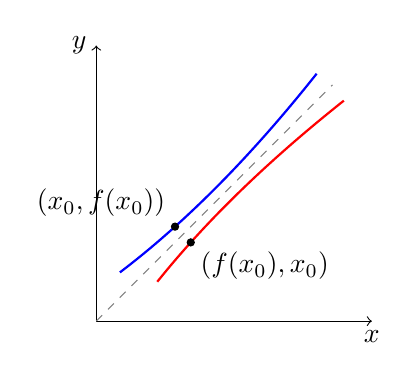
\begin{tikzpicture}[xscale=1.0]
	\draw[->] (0,0) -- (3.5,0) node[below] {$x$};
	\draw[->] (0,0) -- (0,3.5) node[left] {$y$};
	\draw[dashed,gray] (0,0)--(3,3);
	\draw[blue,thick,domain=0.3:2.8,samples=80] plot (\x,{0.4+0.7*\x+0.1*\x*\x});
	\draw[red,thick,domain=0.5:2.8,samples=80] plot ({0.4+0.7*\x+0.1*\x*\x},{\x});
	\fill (1,1.2) circle (1.5pt); \node[above left] at (1,1.2) {$(x_0, f(x_0))$};
	\fill (1.2,1) circle (1.5pt); \node[below right] at (1.2,1) {$(f(x_0), x_0)$};
	\end{tikzpicture}
\caption{Inverse.}
\label{fig:inverse}
\end{figure}

\subsection{Integration theorems}

\begin{proof}[Proof of \autoref{lem:barrow-area}]
For $\mathrm{d}x>0$, $f(x_0)\le f\le f(x_0+\mathrm{d}x)$ on the interval, so
inscribed/circumscribed rectangles bound $A$: 
\begin{equation*}
f(x_0)\,\mathrm{d}x \le A_{x_0}^{x_0+\mathrm{d}x} \le f(x_0+\mathrm{d}x)\,%
\mathrm{d}x.
\end{equation*}
For $\mathrm{d}x<0$, apply \autoref{eq:oriented-area} to reverse both
sides.\hfill$\square$
\end{proof}

\begin{figure}[]
\centering
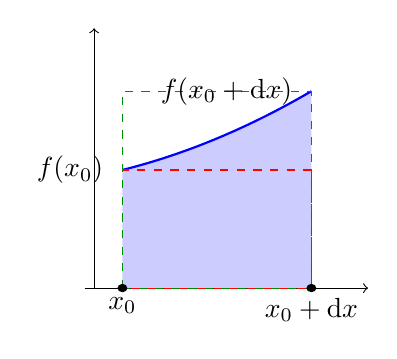
\begin{tikzpicture}[xscale=1.2,yscale=1.0]
	\draw[->] (2.6,0) -- (5.6,0); \draw[->] (2.7,0) -- (2.7,3.3);
	\fill[blue!20] (3,0) -- plot[domain=3:5,samples=60] (\x,{1.5+0.3*(\x-3)+0.1*(\x-3)*(\x-3)}) -- (5,0) -- cycle;
	\draw[blue,thick,domain=3:5,samples=60,smooth] plot (\x,{1.5+0.3*(\x-3)+0.1*(\x-3)*(\x-3)});
	\draw[dashed,red] (3,0) rectangle (5,1.5);
	\draw[dashed,green!55!black] (3,0) rectangle (5,2.5);
	\fill (3,0) circle (1.5pt); \node[below] at (3,0) {$x_0$};
	\fill (5,0) circle (1.5pt); \node[below] at (5,0) {$x_0+\mathrm{d}x$};
	\node[left] at (2.9,1.5) {$f(x_0)$};
	\node[left] at (4.9,2.5) {$f(x_0+\mathrm{d}x)$};
	\end{tikzpicture}
\caption{Barrow's area inequality.}
\label{fig:area-ineq}
\end{figure}

\begin{proof}[Proof of \autoref{lem:mvt-int}]
Define $G(t):=A_{x_0}^{t}$. By FFTC, $G$ is differentiable with $G^{\prime
}=f$.\newline
MVT on the interval with endpoints $x_0$ and $x_0+\mathrm{d}x$ gives $\theta$
between them with 
\begin{equation*}
G^{\prime }(\theta)=\frac{G(x_0+\mathrm{d}x)-G(x_0)}{\mathrm{d}x}.
\end{equation*}
Since $G(x_0)=0$ and $G(x_0+\mathrm{d}x)=A_{x_0}^{x_0+\mathrm{d}x}$, 
\begin{equation*}
A_{x_0}^{x_0+\mathrm{d}x}=f(\theta)\,\mathrm{d}x.
\end{equation*}
\hfill$\square$
\end{proof}

\begin{proof}[Proof of \autoref{thm:fftc}]
Fix $x_0\in(a,b)$ and $\varepsilon>0$. For $h\ne 0$ with $x_0+h\in[a,b]$,
let $I_h$ be the closed interval with endpoints $x_0$ and $x_0+h$. Since $f$
is continuous at $x_0$, for $|h|$ small there exist $m_\varepsilon,M_%
\varepsilon$ with 
\begin{equation*}
m_\varepsilon\le f(u)\le M_\varepsilon\ (u\in I_h), \qquad
|m_\varepsilon-f(x_0)|<\varepsilon, \qquad
|M_\varepsilon-f(x_0)|<\varepsilon.
\end{equation*}
By integral monotonicity applied on $I_h$ to the constants $%
m_\varepsilon,M_\varepsilon$, for $h>0$, 
\begin{equation*}
m_\varepsilon h \le A_{x_0}^{x_0+h} \le M_\varepsilon h;
\end{equation*}
for $h<0$, the same inequality holds with both directions reversed (the
oriented convention \autoref{eq:oriented-area} changes the sign of both $%
A_{x_0}^{x_0+h}$ and $h$). In either case, dividing by $h$ preserves the
direction, giving 
\begin{equation*}
m_\varepsilon \le \frac{A_a^{x_0+h}-A_a^{x_0}}{h} \le M_\varepsilon,
\end{equation*}
where the numerator uses additivity \autoref{eq:lin-int}.\newline
Since $\varepsilon>0$ was arbitrary and $m_\varepsilon,M_\varepsilon\to
f(x_0)$ as $\varepsilon\to 0$, the squeeze theorem yields 
\begin{equation*}
\frac{d}{dx}A_a^{x}\Big|_{x_0}=f(x_0).
\end{equation*}
As $x_0\in(a,b)$ was arbitrary, \autoref{eq:fftc} holds on $(a,b)$; the
one-sided cases follow by one-sided limits.\hfill$\square$
\end{proof}

\noindent\emph{Remark (Barrow's original argument).} Barrow's proof of the
FFTC \cite[Lecture~X, \S 11]{Barrow1916} (see \cite[\S 2--3]{Lopez2026})
assumes \emph{additionally} that $f$ is \emph{increasing}, which makes the
rectangle estimate immediate: for $\mathrm{d}x>0$, 
\begin{equation*}
f(x_0)\,\mathrm{d}x\le A_{x_0}^{x_0+\mathrm{d}x}\le f(x_0+\mathrm{d}x)\,%
\mathrm{d}x,
\end{equation*}
and both inequalities reverse for $\mathrm{d}x<0$ (by \autoref%
{eq:oriented-area}).\newline
Barrow then shows that the line 
\begin{equation*}
L(u)=f(x_0)(u-x_0)+A_a^{x_0},
\end{equation*}
satisfies 
\begin{equation*}
L(x_0+\mathrm{d}x)\le A_a^{x_0+\mathrm{d}x}
\end{equation*}
(respectively $\ge$ for $\mathrm{d}x<0$) and invokes the tangency principle %
\autoref{eq:barrow-tangency} to conclude 
\begin{equation*}
f(x_0)=dA_a^x/dx|_{x_0}.
\end{equation*}
The proof above removes the monotone assumption and uses only continuity via
the squeeze $m_\varepsilon\le (A_a^{x_0+h}-A_a^{x_0})/h\le M_\varepsilon$;
the conclusion is the same.

\begin{figure}[]
\centering
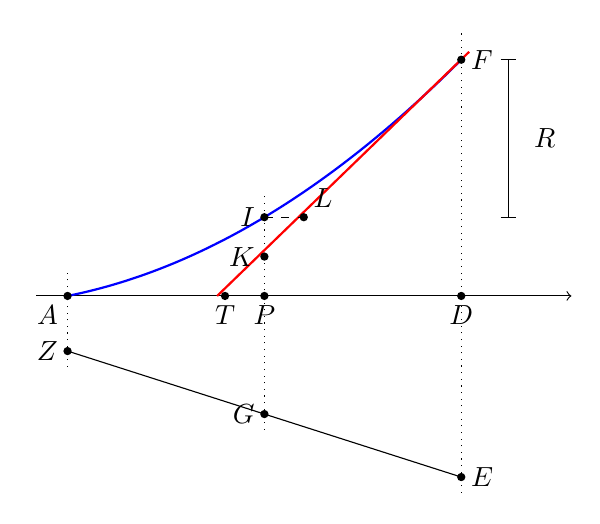
\begin{tikzpicture}[xscale=1.0]
	\draw[->] (-0.4,0) -- (6.4,0);
	\draw[dotted] (0,-0.9) -- (0,0.3);
	\draw[dotted] (2.5,-1.7) -- (2.5,1.3);
	\draw[dotted] (5,-2.5) -- (5,3.4);
	\draw plot[smooth,tension=0.7] coordinates {(0,-0.7) (2.5,-1.5) (5,-2.3)};
	\draw[blue,thick,domain=0:5,samples=100,smooth] plot (\x,{0.08*\x*\x+0.2*\x});
	\draw[red,thick] (1.9,0)--(5.1,3.1);
	\draw[dashed] (2.5,1) -- (3,1);
	\fill (0,0) circle (1.5pt);    \node[below left]  at (0,0)    {$A$};
	\fill (2,0) circle (1.5pt);    \node[below]       at (2,0)    {$T$};
	\fill (2.5,0) circle (1.5pt);  \node[below]       at (2.5,0)  {$P$};
	\fill (5,0) circle (1.5pt);    \node[below]       at (5,0)    {$D$};
	\fill (0,-0.7) circle (1.5pt); \node[left]        at (0,-0.7) {$Z$};
	\fill (2.5,-1.5) circle (1.5pt);\node[left]       at (2.5,-1.5){$G$};
	\fill (5,-2.3) circle (1.5pt); \node[right]       at (5,-2.3) {$E$};
	\fill (2.5,1) circle (1.5pt);  \node[left]        at (2.5,1)  {$I$};
	\fill (2.5,0.5) circle (1.5pt);\node[left]        at (2.5,0.5){$K$};
	\fill (3,1) circle (1.5pt);    \node[above right] at (3,1)    {$L$};
	\fill (5,3) circle (1.5pt);    \node[right]       at (5,3)    {$F$};
	\draw (5.5,1) -- (5.7,1); \draw (5.5,3) -- (5.7,3); \draw (5.6,1) -- (5.6,3);
	\node[right] at (5.8,2) {$R$};
	\end{tikzpicture}
\caption{Barrow's Fig.~109.}
\label{fig:barrow109}
\end{figure}

\begin{proof}[Proof of \autoref{thm:second-ftc}]
Define $G(x):=\int_a^x f$. By FFTC, $G^{\prime }=f$, so $(F-G)^{\prime }=0$
and hence $F-G$ is constant. Therefore 
\begin{equation*}
F(b)-F(a)=\int_a^b f.
\end{equation*}
\hfill$\square$
\end{proof}

\begin{figure}[]
\centering
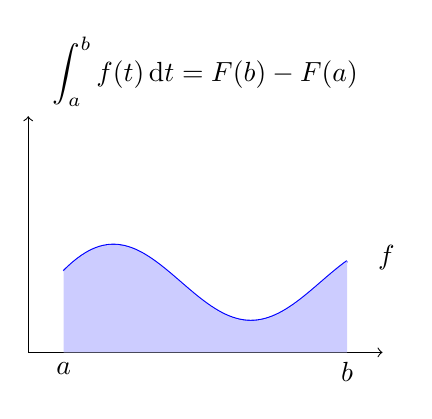
\begin{tikzpicture}[xscale=0.9]
	\draw[->] (0,0) -- (5,0); \draw[->] (0,0) -- (0,3);
	\draw[blue,thick,domain=0.5:4.5,samples=80] plot (\x,{0.5+0.6*sin(\x*1.5 r)+0.5*sin(\x*0.5 r)});
	\fill[blue!20] (0.5,0) -- plot[domain=0.5:4.5,samples=80] (\x,{0.5+0.6*sin(\x*1.5 r)+0.5*sin(\x*0.5 r)}) -- (4.5,0) -- cycle;
	\node[above] at (2.5,3) {$\displaystyle \int_a^b f(t)\,\mathrm{d}t = F(b)-F(a)$};
	\node[below] at (0.5,0) {$a$}; \node[below] at (4.5,0) {$b$};
	\node[right] at (4.8,1.2) {$f$};
	\end{tikzpicture}
\caption{Second FTC.}
\label{fig:second-ftc}
\end{figure}

\begin{proof}[Proof of \autoref{thm:ibp}]
The product rule gives 
\begin{equation*}
(fg)^{\prime }=f^{\prime }g+fg^{\prime }.
\end{equation*}
Integrating with the Second FTC, 
\begin{equation*}
[fg]_a^b =\int_a^b (fg)^{\prime } =\int_a^b f^{\prime }g+\int_a^b fg^{\prime
}.
\end{equation*}
Rearranging, 
\begin{equation*}
\int_a^b f\,g^{\prime }=[fg]_a^b-\int_a^b f^{\prime }\,g.
\end{equation*}
\hfill$\square$
\end{proof}

\begin{proof}[Proof of \autoref{thm:subst}]
Let $F^{\prime }=f$. By the chain rule, 
\begin{equation*}
(F\circ g)^{\prime }=f(g)\,g^{\prime }.
\end{equation*}
Applying the Second FTC on both sides gives 
\begin{equation*}
\int_a^b f(g)\,g^{\prime } =F(g(b))-F(g(a)) =\int_{g(a)}^{g(b)}f.
\end{equation*}
\hfill$\square$
\end{proof}

\begin{proof}[Proof of \autoref{thm:weighted-mvt}]
Since $m\le f\le M$ and $w\ge 0$, 
\begin{equation*}
m\int_a^b w \le\int_a^b fw \le M\int_a^b w.
\end{equation*}
So $A:=\int_a^b fw\big/\int_a^b w\in[m,M]$; by IVT, 
\begin{equation*}
f(c)=A,
\end{equation*}
i.e.\ $\int_a^b fw=f(c)\int_a^b w$.\hfill$\square$
\end{proof}

\subsection{The logarithm and the exponential}

\begin{proof}[Proof of \autoref{thm:log}]
We have 
\begin{equation*}
\ln(ab)-\ln(b)=\int_b^{ab}\frac{\mathrm{d}t}{t}.
\end{equation*}
The substitution $(t,y)\mapsto(t/b,by)$ preserves both area and the identity 
$y=1/t$, so 
\begin{equation*}
\int_b^{ab}\frac{\mathrm{d}t}{t} =\int_1^{a}\frac{\mathrm{d}u}{u} =\ln(a).
\end{equation*}
Hence $\ln(ab)-\ln(b)=\ln(a)$, i.e.\ $\ln(a)+\ln(b)=\ln(ab)$.\hfill$\square$
\end{proof}

\begin{figure}[]
\centering
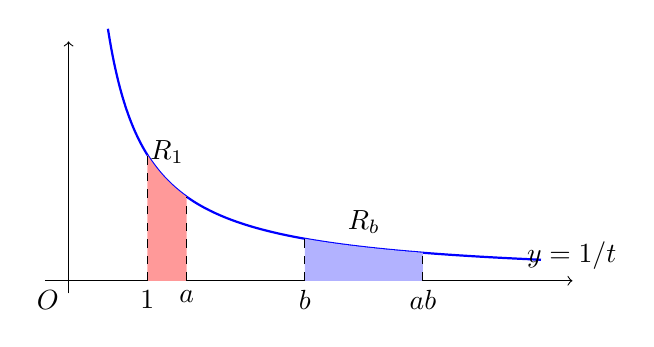
\begin{tikzpicture}[xscale=1.0,yscale=1.6]
	\draw[->] (-0.3,0) -- (6.4,0); \draw[->] (0,-0.1) -- (0,1.9);
	\draw[blue,thick,domain=0.5:6,samples=150,smooth] plot (\x,{1/\x});
	\fill[red!40] (1,0) -- plot[domain=1:1.5,samples=30] (\x,{1/\x}) -- (1.5,0) -- cycle;
	\fill[blue!30] (3,0) -- plot[domain=3:4.5,samples=30] (\x,{1/\x}) -- (4.5,0) -- cycle;
	\draw[dashed] (1,0) -- (1,1); \draw[dashed] (1.5,0) -- (1.5,0.667);
	\draw[dashed] (3,0) -- (3,0.333); \draw[dashed] (4.5,0) -- (4.5,0.222);
	\node[below] at (1,0) {$1$}; \node[below] at (1.5,0) {$a$};
	\node[below] at (3,0) {$b$}; \node[below] at (4.5,0) {$ab$};
	\node[above] at (1.25,0.85) {$R_1$};
	\node[above] at (3.75,0.30) {$R_b$};
	\node[right] at (5.7,0.20) {$y=1/t$};
	\node[below left] at (0,0) {$O$};
	\end{tikzpicture}
\caption{Hyperbolic similarity.}
\label{fig:hyperbola}
\end{figure}

\begin{proof}[Proof of \autoref{thm:exp}]
Since $\ln$ is injective, it suffices to show 
\begin{equation*}
\ln\bigl(\exp(u)\exp(v)\bigr) =\ln(\exp u)+\ln(\exp v) =u+v =\ln\bigl(%
\exp(u+v)\bigr).
\end{equation*}
Injectivity of $\ln$ then gives 
\begin{equation*}
\exp(u)\,\exp(v)=\exp(u+v).
\end{equation*}
\hfill$\square$
\end{proof}

\begin{proof}[Proof of \autoref{thm:image}]
The Sign-Law gives 
\begin{equation*}
\exp(\R_{<0})={]}0,1[, \qquad \exp(\{0\})=\{1\}, \qquad \exp(\R_{>0})={]}%
1,+\infty[.
\end{equation*}
The Image-Union law then gives $\exp(\R)=\R_{>0}$, and bijectivity of $\ln$
gives $\ln(\R_{>0})=\R$.\hfill$\square$
\end{proof}

\begin{figure}[]
\centering
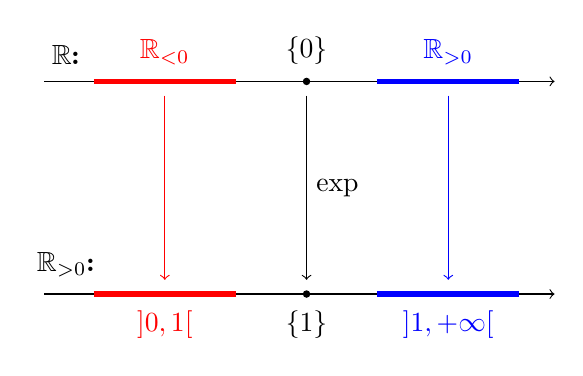
\begin{tikzpicture}[xscale=0.9,yscale=0.9]
	\draw[->] (-0.2,0) -- (7,0);
	\node[above] at (0.1,0.1) {$\R$:};
	\draw[red,line width=2pt] (0.5,0)--(2.5,0);
	\node[above] at (1.5,0.1) {\textcolor{red}{$\R_{<0}$}};
	\fill (3.5,0) circle (1.5pt);
	\node[above] at (3.5,0.1) {$\{0\}$};
	\draw[blue,line width=2pt] (4.5,0)--(6.5,0);
	\node[above] at (5.5,0.1) {\textcolor{blue}{$\R_{>0}$}};
	\draw[->,red]  (1.5,-0.2) -- (1.5,-2.8);
	\draw[->]      (3.5,-0.2) -- (3.5,-2.8);
	\draw[->,blue] (5.5,-0.2) -- (5.5,-2.8);
	\node[right] at (3.5,-1.5) {$\exp$};
	\draw[->] (-0.2,-3) -- (7,-3);
	\node[above] at (0.1,-2.9) {$\R_{>0}$:};
	\draw[red,line width=2pt] (0.5,-3)--(2.5,-3);
	\node[below] at (1.5,-3.1) {\textcolor{red}{${]}0,1[$}};
	\fill (3.5,-3) circle (1.5pt);
	\node[below] at (3.5,-3.1) {$\{1\}$};
	\draw[blue,line width=2pt] (4.5,-3)--(6.5,-3);
	\node[below] at (5.5,-3.1) {\textcolor{blue}{${]}1,+\infty[$}};
	\end{tikzpicture}
\caption{Image of Exponential Function $\exp$}
\label{fig:exp-image}
\end{figure}

\section{Remarks on the geometric development}

Barrow's sliding-tangent MVT proof is retained for its historical content;
the Barrow-tangency principle \autoref{eq:barrow-tangency} is eliminable via
Rolle and Monotone + MVT. The FFTC proof uses only area additivity \autoref%
{eq:lin-int} and rectangle comparison \autoref{eq:barrow-area}; no
Riemann-sum limit is invoked,\,\allowbreak as emphasized by Barrow \cite%
{Barrow1916} and confirmed in \autoref{part:part2}.

\subsection*{Dependency summary}

EVT,\,\allowbreak IVT $\to$ Fermat $\to$ Rolle $\to$ MVT $\to$
Const,\,\allowbreak Monotone,\,\allowbreak Cauchy,\,\allowbreak
Darboux,\,\allowbreak Taylor,\,\allowbreak Convexity,\,\allowbreak Inverse.
Second FTC from FFTC + Const. IBP,\,\allowbreak Subst,\,\allowbreak Weighted
MVT from Second FTC or IVT/IntMono. Log from IntAdd + Similarity; Exp from
Log; Image from LnBij + Sign-Law + ImgUnion. Barrow-area + MVTInt $\to$ FFTC 
$\to$ Log.

\part{\texorpdfstring{Reverse-Mathematical Analysis
in
$\mathsf{RCA}_0$}{Reverse-Mathematical Analysis in RCA0}}

\label{part:part2} \noindent Every \autoref{part:part1} entry reappears as a
tagged statement with a dependency table and an exact strength in $\{\mathsf{%
FOL},\,\allowbreak\mathsf{RCA}_0,\,\allowbreak\mathsf{WKL}_0,\,\allowbreak%
\mathsf{ACA}_0,\,\allowbreak\mathsf{ZF},\,\allowbreak\mathsf{ZFC}\}$.
Geometric proofs are at most $\mathsf{WKL}_0$ as written; \S \ref%
{sec:core-proofs} gives the matching $\mathsf{RCA}_0$-strength tables via
Hardin--Velleman,\,\allowbreak Yokoyama,\,\allowbreak or direct argument.

\section{Coding conventions}

\label{sec:coding}

\noindent Following Yokoyama \cite{Yokoyama2010},\,\allowbreak we
distinguish:

\begin{itemize}
\item \emph{Pointwise differentiability:} the limit exists for each $x\in I$%
; no derivative function needed. Hardin--Velleman's Rolle and MVT in $%
\mathsf{RCA}_0$ use this.

\item \emph{Strong $C^k$-coding:} $C^k_{\mathrm{strong}}(I)(f):\iff\exists
g_0,\,\allowbreak\dots,\,\allowbreak g_k:\ g_0=f\wedge\forall
j<k,\,\allowbreak\ g_{j+1}=g_j^{\prime }$. All $C^k$ hypotheses in \autoref%
{part:part2} mean strong $C^k$-coding.

\item \emph{Inverse function:} Yokoyama \cite[Thm.~3.22]{Yokoyama2010} in $%
\mathsf{RCA}_0$ for strong $C^1$-functions with $f^{\prime }\ne0$ on $I$%
,\,\allowbreak $x_0\in I^\circ$. The pointwise form is not $\mathsf{RCA}_0$%
-provable.
\end{itemize}

\section{Research context}

\label{sec:research}

\subsection{The core hierarchy}

$\mathsf{RCA}_0$ = recursive comprehension + $\Sigma^0_1$-induction; no
choice.

\begin{center}
{\small \ \noindent%
\begin{tabular}{|>{\raggedright\arraybackslash}m{4.5cm}|>{\centering\arraybackslash}m{2.2cm}|>{\centering\arraybackslash}m{3.2cm}|>{\centering\arraybackslash}m{1.3cm}|}
\hline
\textbf{Result} & \textbf{Strength} & \textbf{Reference} & \textbf{Choice}
\\ \hline
\textsf{MVT} & \textsf{RCA$_0$} & \cite{HardinVelleman2001} & \textsf{none}
\\ \hline
\textsf{IVT},\,\allowbreak \textsf{EVT} & \textsf{WKL$_0$} & \cite%
{Simpson2009} & \textsf{none} \\ \hline
\textsf{sequential IVT/MVT} & $\equiv\mathsf{WKL}_0$ & \cite%
{Simpson2009,Sanders2020} & \textsf{none} \\ \hline
$\ln$/$\exp$ chain & \textsf{RCA$_0$} & \cite{Yokoyama2010} & \textsf{none}
\\ \hline
\end{tabular}
}
\end{center}

\noindent Key facts:

\begin{itemize}
\item \textbf{MVT $\in\mathsf{RCA}_0$} (Hardin--Velleman \cite%
{HardinVelleman2001}); no EVT,\,\allowbreak no IVT.

\item \textbf{IVT $\equiv\mathsf{WKL}_0$}: sole non-$\mathsf{RCA}_0$
ingredient is $\sup\{x:f(x)<0\}$.

\item \textbf{Inverse function $\in\mathsf{RCA}_0$} (Yokoyama \cite[Thm.~3.22%
]{Yokoyama2010}).

\item \textbf{$\ln$/$\exp$ $\in\mathsf{RCA}_0$}: definitional plus integral
postulates.
\end{itemize}

\setcounter{theorem}{0}

\begin{remark}[Proofs vs.\ classification]
\autoref{part:part1} proofs use $\sup$,\,\allowbreak $\inf$,\,\allowbreak
LUB (\textsf{ax:R-complete}). MVT is $\mathsf{RCA}_0$ via Hardin--Velleman.
IVT,\,\allowbreak EVT are $\mathsf{WKL}_0$-equivalent over $\mathsf{RCA}_0$
and remain $\mathsf{WKL}_0$.
\end{remark}

\subsection{Illustrative theorems}

\bigskip

\begin{center}
{\small \ 
\begin{tabular}{|>{\raggedright\arraybackslash}m{4.5cm}|>{\centering\arraybackslash}m{2.5cm}|>{\centering\arraybackslash}m{3.2cm}|>{\centering\arraybackslash}m{1.3cm}|}
\hline
\textbf{Theorem} & \textbf{Strength} & \textbf{Reference} & \textbf{Choice}
\\ \hline
\textsf{IVT} & \textsf{WKL$_0$} & \cite{Simpson2009} & \textsf{none} \\ 
\hline
\textsf{MVT} & \textsf{RCA$_0$} & \cite{HardinVelleman2001} & \textsf{none}
\\ \hline
\textsf{Hahn--Banach} & $\equiv\mathsf{WKL}_0$ & \cite{Simpson2009} & 
\textsf{none} \\ \hline
\textsf{Weierstrass approx.} & $\equiv\mathsf{WKL}_0$ & \cite{Simpson2009} & 
\textsf{none} \\ \hline
\textsf{Peano existence} & $\equiv\mathsf{WKL}_0$ & \cite{Simpson2009} & 
\textsf{none} \\ \hline
\textsf{sequential IVT/MVT} & $\equiv\mathsf{WKL}_0$ & \cite{Sanders2020} & 
\textsf{none} \\ \hline
\textsf{separation} & $\equiv\mathsf{ACA}_0$ & \cite{Humphreys2015} & 
\textsf{none} \\ \hline
\textsf{Banach--Alaoglu} & \textsf{ZFC} & \cite{Alaoglu1940} & \textsf{full
AC} \\ \hline
\textsf{Tychonoff} & \textsf{ZFC} & \cite{Kelley1950} & \textsf{full AC} \\ 
\hline
\textsf{well-ordering} & \textsf{ZFC} & \cite{Jech1973} & \textsf{full AC}
\\ \hline
\end{tabular}
}
\end{center}

\medskip \noindent Strictness: $\mathsf{RCA}_0\subsetneq\mathsf{WKL}%
_0\subsetneq\mathsf{ACA}_0\subsetneq\mathsf{ZFC}$.

\subsection{Dedekind vs.\ Cauchy completeness}

\begin{itemize}
\item \textbf{Dedekind (LUB):} every nonempty bounded-above subset has a
supremum. A $\mathsf{ZF}$ theorem; equivalent over ordered fields to
IVT,\,\allowbreak EVT,\,\allowbreak MVT,\,\allowbreak Darboux \cite%
{Propp2012,Teismann2013}. Form used here: \textsf{ax:R-complete}.

\item \textbf{Cauchy completeness:} every Cauchy sequence converges. $%
\mathsf{ZF}$-equivalent to $\mathsf{DC}_\R$. Not a $\mathsf{ZF}$ theorem.
Not used here.
\end{itemize}

Solovay's model \cite{Solovay1970}: under $\mathsf{ZF}+\mathsf{DC}$%
,\,\allowbreak all reals are Lebesgue measurable and $\mathsf{AC}$ fails; $%
\mathsf{DC}\Rightarrow\mathsf{DC}_\R$,\,\allowbreak so Cauchy completeness
holds there. The choice-free classification is strictly finer than $\mathsf{%
DC}_\R$.

\subsection{Constructive RM}

In BISH,\,\allowbreak IVT $\equiv\mathsf{LLPO}$ \cite{Bridges2023}. This
document is classical.

\subsection{Lean~4 and Mathlib}

Lean~4 and Mathlib \cite{Lean4}: about $70.4\%$ of declarations depend
syntactically on \textsf{Classical.choice},\,\allowbreak of which roughly
half reach it only through classical logic (law of excluded
middle,\,\allowbreak \textsf{propext},\,\allowbreak \textsf{Quot.sound})
rather than through genuine choice; $13.1\%$ have choice-free statements
with choice-dependent proofs \cite{Crossref2026}. Our classification is
stronger: it certifies choice-free proofs,\,\allowbreak not just statements.

\section{Axioms}

\label{sec:axioms}

\noindent The fourteen axioms of $\R$ as a complete ordered field.

\medskip

\noindent$%
\begin{array}{|C|L|R|C|}
\hline
\refstepcounter{axctr}\hypertarget{ax:R-add-assoc}{\mbox{\textbf{Ax\,\theaxctr}}}\label{axi:R-add-assoc} &
\textsf{ax{:}add{-}assoc}:\forall (x,\,\allowbreak y,\,\allowbreak z:\R),\,\allowbreak\;(x+y)+z=x+(y+z) &
\textsf{Add.}\allowbreak\textsf{Assoc.} & $\textsf{ZF}$ \\ \hline
\refstepcounter{axctr}\hypertarget{ax:R-add-comm}{\mbox{\textbf{Ax\,\theaxctr}}}\label{axi:R-add-comm} &
\textsf{ax{:}add{-}comm}:\forall (x,\,\allowbreak y:\R),\,\allowbreak\;x+y=y+x &
\textsf{Add.}\allowbreak\textsf{Comm.} & $\textsf{ZF}$ \\ \hline
\end{array}$

\nointerlineskip\noindent$%
\begin{array}{|C|L|R|C|}
\hline
\refstepcounter{axctr}\hypertarget{ax:R-add-zero}{\mbox{\textbf{Ax\,\theaxctr}}}\label{axi:R-add-zero} &
\textsf{ax{:}add{-}zero}:\forall (x:\R),\,\allowbreak\;0+x=x &
\textsf{Add.}\allowbreak\textsf{Id.} & $\textsf{ZF}$ \\ \hline
\refstepcounter{axctr}\hypertarget{ax:R-add-inv}{\mbox{\textbf{Ax\,\theaxctr}}}\label{axi:R-add-inv} &
\textsf{ax{:}add{-}inv}:\forall (x:\R),\,\allowbreak\;x+(-x)=0 &
\textsf{Add.}\allowbreak\textsf{Inv.} & $\textsf{ZF}$ \\ \hline
\end{array}$

\nointerlineskip\noindent$%
\begin{array}{|C|L|R|C|}
\hline
\refstepcounter{axctr}\hypertarget{ax:R-mul-assoc}{\mbox{\textbf{Ax\,\theaxctr}}}\label{axi:R-mul-assoc} &
\textsf{ax{:}mul{-}assoc}:\forall (x,\,\allowbreak y,\,\allowbreak z:\R),\,\allowbreak\;(x\cdot y)\cdot z=x\cdot(y\cdot z) &
\textsf{Mul.}\allowbreak\textsf{Assoc.} & $\textsf{ZF}$ \\ \hline
\refstepcounter{axctr}\hypertarget{ax:R-mul-comm}{\mbox{\textbf{Ax\,\theaxctr}}}\label{axi:R-mul-comm} &
\textsf{ax{:}mul{-}comm}:\forall (x,\,\allowbreak y:\R),\,\allowbreak\;x\cdot y=y\cdot x &
\textsf{Mul.}\allowbreak\textsf{Comm.} & $\textsf{ZF}$ \\ \hline
\end{array}$

\nointerlineskip\noindent$%
\begin{array}{|C|L|R|C|}
\hline
\refstepcounter{axctr}\hypertarget{ax:R-mul-one}{\mbox{\textbf{Ax\,\theaxctr}}}\label{axi:R-mul-one} &
\textsf{ax{:}mul{-}one}:\forall (x:\R),\,\allowbreak\;1\cdot x=x &
\textsf{Mul.}\allowbreak\textsf{Id.} & $\textsf{ZF}$ \\ \hline
\refstepcounter{axctr}\hypertarget{ax:R-mul-inv}{\mbox{\textbf{Ax\,\theaxctr}}}\label{axi:R-mul-inv} &
\textsf{ax{:}mul{-}inv}:\forall (x:\R),\,\allowbreak\;(x\ne0\to x\cdot x^{-1}=1)\wedge(x=0\to x^{-1}=0) &
\textsf{Mul.}\allowbreak\textsf{Inv.} & $\textsf{ZF}$ \\ \hline
\end{array}$

\nointerlineskip\noindent$%
\begin{array}{|C|L|R|C|}
\hline
\refstepcounter{axctr}\hypertarget{ax:R-distrib}{\mbox{\textbf{Ax\,\theaxctr}}}\label{axi:R-distrib} &
\textsf{ax{:}distrib}:\forall (x,\,\allowbreak y,\,\allowbreak z:\R),\,\allowbreak\;x\cdot(y+z)=x\cdot y+x\cdot z &
\textsf{Distrib.} & $\textsf{ZF}$ \\ \hline
\refstepcounter{axctr}\hypertarget{ax:R-nontriv}{\mbox{\textbf{Ax\,\theaxctr}}}\label{axi:R-nontriv} &
\textsf{ax{:}nontriv}:0\ne1 &
\textsf{Nontriv.} & $\textsf{ZF}$ \\ \hline
\end{array}$

\nointerlineskip\noindent$%
\begin{array}{|C|L|R|C|}
\hline
\refstepcounter{axctr}\hypertarget{ax:R-order}{\mbox{\textbf{Ax\,\theaxctr}}}\label{axi:R-order} &
\textsf{ax{:}order}:\bigl(\forall x:\,x\le x\bigr)\wedge\bigl(\forall x,\,\allowbreak y:\,x\le y\wedge y\le x\to x=y\bigr)\wedge\bigl(\forall x,\,\allowbreak y,\,\allowbreak z:\,x\le y\wedge y\le z\to x\le z\bigr)\wedge\bigl(\forall x,\,\allowbreak y:\,x\le y\vee y\le x\bigr) &
\textsf{Linear}\allowbreak\textsf{Order} & $\textsf{ZF}$ \\ \hline
\refstepcounter{axctr}\hypertarget{ax:R-add-monotone}{\mbox{\textbf{Ax\,\theaxctr}}}\label{axi:R-add-monotone} &
\textsf{ax{:}add{-}mon}:\forall (x,\,\allowbreak y,\,\allowbreak z:\R),\,\allowbreak\;x\le y\to x+z\le y+z &
\textsf{Add}\allowbreak\textsf{Mon.} & $\textsf{ZF}$ \\ \hline
\end{array}$

\nointerlineskip\noindent$%
\begin{array}{|C|L|R|C|}
\hline
\refstepcounter{axctr}\hypertarget{ax:R-mul-monotone-pos}{\mbox{\textbf{Ax\,\theaxctr}}}\label{axi:R-mul-monotone-pos} &
\textsf{ax{:}mul{-}mon}:\forall (x,\,\allowbreak y:\R),\,\allowbreak\;0\le x\wedge0\le y\to0\le x\cdot y &
\textsf{Mul}\allowbreak\textsf{Mon.} & $\textsf{ZF}$ \\ \hline
\refstepcounter{axctr}\hypertarget{ax:R-complete}{\mbox{\textbf{Ax\,\theaxctr}}}\label{axi:R-complete} &
\textsf{ax{:}complete}:\bigl(\exists x,\,\allowbreak S(x)\bigr)\wedge\bigl(\exists u,\,\allowbreak\forall x,\,\allowbreak S(x)\to x\le u\bigr)\to\exists s,\,\allowbreak\bigl(\forall x,\,\allowbreak S(x)\to x\le s\bigr)\wedge\bigl(\forall u,\,\allowbreak(\forall x,\,\allowbreak S(x)\to x\le u)\to s\le u\bigr) &
\textsf{Cut} & $\textsf{ZF}$ \\ \hline
\end{array}$

\medskip

\medskip

\noindent The fourteen axioms of $\R$ as a complete ordered field are listed
above. Only the first thirteen are used in \autoref{part:part2}; the
fourteenth, \textsf{ax:R-complete} (Cut), enters no \autoref{part:part2}
proof. It is $\mathsf{ZF}$-realizable via Dedekind cuts without choice.

\section{Postulates}

\label{sec:postulates}

\noindent Unproved internal statements. Each is $\mathsf{RCA}_0$-provable or
first-order logical; none introduces choice.

\subsection{Integral postulates}

\noindent$%
\begin{array}{|C|L|R|C|}
\hline
\refstepcounter{posctr}\hypertarget{pos:int-linear}{\mbox{\textbf{Pos\,\theposctr}}}\label{posi:int-linear} &
\textsf{Pos{:}IntLinear}:\forall (a,b:\R),\;\forall (f,g\in L^{1}([a,b])),\;\forall (\alpha,\beta:\R),\;\int_{a}^{b}(\alpha f(x)+\beta g(x))\,dx=\alpha\int_{a}^{b}f(x)\,dx+\beta\int_{a}^{b}g(x)\,dx &
\textsf{IntLin} & $\textsf{RCA}_0$ \\ \hline
\refstepcounter{posctr}\hypertarget{pos:int-add}{\mbox{\textbf{Pos\,\theposctr}}}\label{posi:int-add} &
\textsf{Pos{:}IntAdd}:\forall (a,b,c:\R),\;\forall (f\in L^{1}([\min(a,b,c),\max(a,b,c)])),\;\int_{a}^{b}f(x)\,dx=\int_{a}^{c}f(x)\,dx+\int_{c}^{b}f(x)\,dx &
\textsf{IntAdd} & $\textsf{RCA}_0$ \\ \hline
\end{array}$ \medskip \text{ \ } \newline

\noindent{\footnotesize \textsf{Note:} $f\in L^1([\alpha,\beta])$ and $%
[\gamma,\delta]\subseteq[\alpha,\beta]$ imply $f\in L^1([\gamma,\delta])$;
cited as \texttt{restrict} in proof tables.}

\nointerlineskip\noindent$%
\begin{array}{|C|L|R|C|}
\hline
\refstepcounter{posctr}\hypertarget{pos:int-mono}{\mbox{\textbf{Pos\,\theposctr}}}\label{posi:int-mono} &
\textsf{Pos{:}IntMono}:\forall (a,b:\R),\;a<b\to\forall (f,g\in L^{1}([a,b])),\;\bigl(\forall (x\in[a,b]),\;f(x)\le g(x)\bigr)\to\int_{a}^{b}f(x)\,dx\le\int_{a}^{b}g(x)\,dx &
\textsf{IntMono} & $\textsf{RCA}_0$ \\ \hline
\refstepcounter{posctr}\hypertarget{pos:int-subst}{\mbox{\textbf{Pos\,\theposctr}}}\label{posi:int-subst} &
\textsf{Pos{:}IntSubst}:\forall (a,b:\R),\;\forall (g:\R\to\R),\;\forall (f:\R\to\R),\;
g\in C^{1}([\min(a,b),\max(a,b)])\wedge
\bigl(\forall t\in[\min(a,b),\max(a,b)],\;g^{\prime}(t)\neq0\bigr)\wedge
f\in C^{0}(g([\min(a,b),\max(a,b)]))
\to\int_{g(a)}^{g(b)}f(x)\,dx=\int_{a}^{b}f(g(t))\,g^{\prime}(t)\,dt &
\textsf{IntSubst} & $\textsf{RCA}_0$ \\ \hline
\end{array}$

\nointerlineskip\noindent$%
\begin{array}{|C|L|R|C|}
\hline
\refstepcounter{posctr}\hypertarget{pos:int-cont-integ}{\mbox{\textbf{Pos\,\theposctr}}}\label{posi:int-cont-integ} &
\textsf{Pos{:}ContInt}:\forall (a,b:\R),\;a<b\to\forall (f:\R\to\R),\;f\in C^{0}([a,b])\to f\in L^{1}([a,b]) &
\textsf{ContInt} & $\textsf{RCA}_0$ \\ \hline
\refstepcounter{posctr}\hypertarget{pos:similarity}{\mbox{\textbf{Pos\,\theposctr}}}\label{posi:similarity} &
\textsf{Pos{:}Similarity}:\forall (a,b:\R),\;0<a\wedge0<b\to\forall (h:\R\to\R),\;\int_{b}^{a\cdot b}h(t)\,dt=\int_{1}^{a}h(bu)\cdot b\,du&
\textsf{Sim.} & $\textsf{RCA}_0$ \\ \hline
\end{array}$

\subsection{Differential postulates}

\noindent$%
\begin{array}{|C|L|R|C|}
\hline
\refstepcounter{posctr}\hypertarget{pos:prod-rule}{\mbox{\textbf{Pos\,\theposctr}}}\label{posi:prod-rule} &
\textsf{Pos{:}ProdRule}:\forall (f,g:\R\to\R),\;\forall (x:\R),\;\mathsf{Diff}(f,x)\wedge\mathsf{Diff}(g,x)\to\mathsf{Diff}(f\cdot g,x)\wedge(f\cdot g)^{\prime}(x)=f^{\prime}(x)g(x)+f(x)g^{\prime}(x) &
\textsf{Prod} & $\textsf{RCA}_0$ \\ \hline
\refstepcounter{posctr}\hypertarget{pos:chain-rule}{\mbox{\textbf{Pos\,\theposctr}}}\label{posi:chain-rule} &
\textsf{Pos{:}ChainRule}:\forall (f,g:\R\to\R),\;\forall (x:\R),\;\mathsf{Diff}(g,x)\wedge\mathsf{Diff}(f,g(x))\to\mathsf{Diff}(f\circ g,x)\wedge(f\circ g)^{\prime}(x)=f^{\prime}(g(x))\cdot g^{\prime}(x) &
\textsf{Chain} & $\textsf{RCA}_0$ \\ \hline
\end{array}$

\nointerlineskip\noindent$%
\begin{array}{|C|L|R|C|}
\hline
\refstepcounter{posctr}\hypertarget{pos:inv-cont}{\mbox{\textbf{Pos\,\theposctr}}}\label{posi:inv-cont} &
\textsf{Pos{:}InvCont}:\bigl(t\mapsto1/t\bigr)\in C^{0}(\R_{>0}) &
\textsf{InvCont} & $\textsf{RCA}_0$ \\ \hline
\refstepcounter{posctr}\hypertarget{pos:barrow-tangency}{\mbox{\textbf{Pos\,\theposctr}}}\label{posi:barrow-tangency} &
\textsf{Pos{:}BarrowTangency}:\forall (G:\R\to\R),\;\forall (x_0,m:\R),\;\mathsf{Diff}(G,x_0)\wedge
\Bigl(\bigl(\forall (u\neq x_0)\ \text{near}\ x_0,\;G(x_0)+m(u-x_0)\le G(u)\bigr)\vee
\bigl(\forall (u\neq x_0)\ \text{near}\ x_0,\;G(x_0)+m(u-x_0)\ge G(u)\bigr)\Bigr)\to m=G^{\prime}(x_0) &
\textsf{Barrow} & $\textsf{RCA}_0$ \\ \hline
\end{array}$

\subsection{Logarithmic postulates}

\noindent$%
\begin{array}{|C|L|R|C|}
\hline
\refstepcounter{posctr}\hypertarget{pos:ln-bij}{\mbox{\textbf{Pos\,\theposctr}}}\label{posi:ln-bij} &
\textsf{Pos{:}LnBij}:\mathsf{Bijective}(\ln:\R_{>0}\to\R) &
\textsf{LnBij} & $\textsf{RCA}_0$ \\ \hline
\refstepcounter{posctr}\hypertarget{pos:ln-sign}{\mbox{\textbf{Pos\,\theposctr}}}\label{posi:ln-sign} &
\textsf{Pos{:}LnSign}:\forall (a:\R_{>0}),\;
\bigl(\ln(a)<0\leftrightarrow a<1\bigr)\wedge
\bigl(\ln(a)=0\leftrightarrow a=1\bigr)\wedge
\bigl(\ln(a)>0\leftrightarrow a>1\bigr) &
\textsf{LnSign} & $\textsf{RCA}_0$ \\ \hline
\end{array}$

\subsection{Logical postulate}

\noindent$%
\begin{array}{|C|L|R|C|}
\hline
\refstepcounter{posctr}\hypertarget{pos:img-union}{\mbox{\textbf{Pos\,\theposctr}}}\label{posi:img-union} &
\textsf{Pos{:}ImgUnion}:\forall (X,Y:\mathsf{Type}),\;\forall (f:X\to Y),\;\forall (A,B:X\to\mathsf{Prop}),\;
f(A\cup B)=f(A)\cup f(B) &
\textsf{ImgUnion} & $\textsf{FOL}$ \\ \hline
\end{array}$

\subsection{External results}

\noindent$%
\begin{array}{|C|L|R|C|}
\hline
\refstepcounter{posctr}\hypertarget{pos:cont-img-bdd}{\mbox{\textbf{Pos\,\theposctr}}}\label{posi:cont-img-bdd} &
\textsf{Pos{:}ContImgBdd}:\forall (f:[a,b]\to\R),\ f\in C^{0}([a,b])\to
\bigl(\exists L,U:\R,\ \forall x:[a,b],\ L\le f(x)\le U\bigr) &
\textsf{BddImg} & $\textsf{RCA}_0$ \\ \hline
\refstepcounter{posctr}\hypertarget{pos:cont-img-attain}{\mbox{\textbf{Pos\,\theposctr}}}\label{posi:cont-img-attain} &
\textsf{Pos{:}ContImgAttain}:\forall (f:[a,b]\to\R),\ f\in C^{0}([a,b])\to
\bigl(\exists x_{\max}:[a,b],\forall x:[a,b],f(x)\le f(x_{\max})\bigr)
\wedge\bigl(\exists x_{\min}:[a,b],\forall x:[a,b],f(x_{\min})\le f(x)\bigr) &
\textsf{Attain} & $\textsf{WKL}_0$ \\ \hline
\end{array}$

\text{\ }\medskip

\noindent{\footnotesize \textsf{Note on \textsf{Pos:ContImgBdd} and the
coding of $C^0([a,b])$.} Under the coding of \S \ref{sec:coding} (following
Simpson \cite{Simpson2009}), a continuous function $f:[a,b]\to\R$ carries a
coded modulus of continuity, from which boundedness of the image $f([a,b])$
follows in $\mathsf{RCA}_0$. The \textsf{Pos:ContImgBdd} tag $\mathsf{RCA}_0$
reflects this standard coding convention. Under an alternative coding ---
pointwise continuity without a coded modulus --- boundedness of continuous
functions on $[a,b]$ rises to $\mathsf{WKL}_0$; the choice between codings
is a foundation choice, not a mathematical error, and \S \ref{sec:coding}
fixes the Simpson convention for this document.} \medskip

\nointerlineskip\noindent$%
\begin{array}{|C|L|R|C|}
\hline
\refstepcounter{posctr}\hypertarget{pos:pi01-sup}{\mbox{\textbf{Pos\,\theposctr}}}\label{posi:pi01-sup} &
\textsf{Pos{:}}\Pi^{0}_{1}\textsf{Sup}:\forall (\varphi:\N\times\R\to\{0,1\}),\;\forall (a,b:\R),\;a\le b\to
\bigl(\exists x\in[a,b],\forall n\,\varphi(n,x)=0\bigr)\to
\exists s\in[a,b],\;
\bigl(\forall x\in[a,b],(\forall n\,\varphi(n,x)=0)\to x\le s\bigr)\wedge
\bigl(\forall u\in[a,b],(\forall x\in[a,b],(\forall n\,\varphi(n,x)=0)\to x\le u)\to s\le u\bigr) &
\textsf{Sup} & $\textsf{WKL}_0$ \\ \hline
\refstepcounter{posctr}\hypertarget{pos:sigma01-choice}{\mbox{\textbf{Pos\,\theposctr}}}\label{posi:sigma01-choice} &
\textsf{Pos{:}}\Sigma^{0}_{1}\textsf{Choice}:\bigl(\forall n,\exists m,R(n,m)\bigr)\to\exists g,\forall n,R(n,g(n)) &
\Sigma^0_1 & 
$\textsf{RCA}_0$ \\ \hline
\end{array}$

\nointerlineskip\noindent$%
\begin{array}{|C|L|R|C|}
\hline
\refstepcounter{posctr}\hypertarget{pos:seq-cont}{\mbox{\textbf{Pos\,\theposctr}}}\label{posi:seq-cont} &
\textsf{Pos{:}SeqCont}:\forall (f:[a,b]\to\R),f\in C^{0}([a,b])\to
\forall x:[a,b],\ \forall (x_n:\N\to[a,b]),\ (x_n\to x)\to \bigl(f(x_n)\to f(x)\bigr) &
\textsf{SeqCont} & $\textsf{RCA}_0$ \\ \hline
\refstepcounter{posctr}\hypertarget{pos:hv-rolle}{\mbox{\textbf{Pos\,\theposctr}}}\label{posi:hv-rolle} &
\textsf{Pos{:}HVRolle}:\forall (f:[a,b]\to\R),\;
f\in C^{0}([a,b])\wedge
\bigl(\forall x:(a,b),\ \mathsf{Diff}(f,x)\bigr)\wedge f(a)=f(b)\to
\exists c:(a,b),\ f^{\prime}(c)=0 &
\textsf{HVRolle} & $\textsf{RCA}_0$ \\ \hline
\end{array}$

\nointerlineskip\noindent$%
\begin{array}{|C|L|R|C|}
\hline
\refstepcounter{posctr}\hypertarget{pos:yokoyama-inv}{\mbox{\textbf{Pos\,\theposctr}}}\label{posi:yokoyama-inv} &
\textsf{Pos{:}YokoyamaInv}:\forall (f:I\to\R),\ \forall (x_0:I^{\circ}),\
C^{1}_{\mathrm{strong}}(I)(f)\wedge(\forall x:I,f^{\prime}(x)\neq 0)\wedge\mathsf{StrictMono}(f)\to
\mathsf{Diff}(f^{-1},f(x_0))\wedge(f^{-1})^{\prime}(f(x_0))=1/f^{\prime}(x_0) &
\textsf{YokInv} & $\textsf{RCA}_0$ \\ \hline
\end{array}$

\section{Definitions}

\label{sec:definitions}

\noindent Definitional abbreviations available in $\mathsf{RCA}_0$: set
notation by $\Delta^0_1$-comprehension; $L^1,\,\allowbreak C^k,\,\allowbreak
C^k_{\mathrm{strong}}$ by $\Sigma^0_1$ predicates; $A_a^x,\,\allowbreak\ln,%
\,\allowbreak\exp$ by unique existence + graphs; \textsf{Diff}%
,\,\allowbreak\allowbreak \textsf{ChordSlope},\,\allowbreak\allowbreak%
\textsf{TangentSlope},\,\allowbreak\allowbreak\textsf{LocalExt}%
,\,\allowbreak\allowbreak\textsf{Increasing},\,\allowbreak\textsf{StrictInc}%
,\,\allowbreak\allowbreak\textsf{StrictDec},\,\allowbreak\allowbreak\textsf{%
StrictMono} by definitional extension.

\text{ \ }\newline
\medskip \noindent \noindent$%
\begin{array}{|C|L|R|C|}
\hline
\refstepcounter{defctr}\hypertarget{def:R-pos}{\mbox{\textbf{Def\,\thedefctr}}}\label{defi:R-pos} &
\mathsf{Def{:}R_{>0}}:\R_{>0}:=\{x:\R\mid x>0\},\;\R_{<0}:=\{x:\R\mid x<0\},\;\R_{\geq0}:=\{x:\R\mid x\geq0\} &
\textsf{R}_{\textsf{>0}} & $\textsf{RCA}_0$ \\ \hline
\refstepcounter{defctr}\hypertarget{def:L1}{\mbox{\textbf{Def\,\thedefctr}}}\label{defi:L1} &
\mathsf{Def{:}L^{1}}:L^{1}([a,b]):=\{f:\R\to\R\mid\int_{a}^{b}|f(x)|\,dx<\infty\} &
\textsf{L}^{\textsf{1}} & $\textsf{RCA}_0$ \\ \hline
\end{array}$

\nointerlineskip\noindent$%
\begin{array}{|C|L|R|C|}
\hline
\refstepcounter{defctr}\hypertarget{def:Ck}{\mbox{\textbf{Def\,\thedefctr}}}\label{defi:Ck} &
\mathsf{Def{:}C^{k}}:\forall (k:\N),\;\forall (U:\R\to\mathsf{Prop}),\;C^{k}(U):=\{f:\R\to\R\mid f\;\textsf{k}{-}\mathsf{times}\allowbreak \mathsf{cont.\ diff.\ on}\;U\} &
\textsf{C}^{\textsf{k}} & $\textsf{RCA}_0$ \\ \hline
\refstepcounter{defctr}\hypertarget{def:strong-Ck}{\mbox{\textbf{Def\,\thedefctr}}}\label{defi:strong-Ck} &
\mathsf{Def{:}C^{k}_{\mathrm{strong}}}:\forall (k:\N),\;\forall (I:\R\to\mathsf{Prop}),\;
C^{k}_{\mathrm{strong}}(I)(f):\iff
\exists (g_0,\dots,g_k:\R\to\R),\;
g_0=f\wedge
\bigl(\forall j\le k,\;g_j\in C^{0}(I)\bigr)\wedge
\bigl(\forall j<k,\;g_{j+1}=(g_j)'\bigr)
& \textsf{Strong\ C}^{\textsf{k}} & $\textsf{RCA}_0$ \\ \hline
\end{array}$

\nointerlineskip\noindent$%
\begin{array}{|C|L|R|C|}
\hline
\refstepcounter{defctr}\hypertarget{def:diff}{\mbox{\textbf{Def\,\thedefctr}}}\label{defi:diff} &
\mathsf{Def{:}Diff}:\forall (f:\R\to\R),\;\forall (x:\R),\;\mathsf{Diff}(f,x):\iff\lim_{h\to0}\tfrac{f(x+h)-f(x)}{h}\ \text{exists};\quad f^{\prime}(x):=\text{that limit} &
\textsf{Diff} & $\textsf{RCA}_0$ \\ \hline
\refstepcounter{defctr}\hypertarget{def:area}{\mbox{\textbf{Def\,\thedefctr}}}\label{defi:area} &
\mathsf{Def{:}Area}:\forall (f:\R\to\R),\;\forall (a,x:\R),\;A_{a}^{x}:=\int_{a}^{x}f(t)\,dt\ \text{with}\ A_{x}^{x}=0,\ A_{x}^{x+\mathrm{d}x}=-A_{x+\mathrm{d}x}^{x}\ (\mathrm{d}x<0) &
\textsf{Area} & $\textsf{RCA}_0$ \\ \hline
\end{array}$

\nointerlineskip\noindent$%
\begin{array}{|C|L|R|C|}
\hline
\refstepcounter{defctr}\hypertarget{def:chord}{\mbox{\textbf{Def\,\thedefctr}}}\label{defi:chord} &
\mathsf{Def{:}chord}:\forall (f:\R\to\R),\;\forall (a,b:\R),\;a\neq b\to\mathsf{ChordSlope}(f,a,b):=\tfrac{f(b)-f(a)}{b-a} &
\textsf{Chord} & $\textsf{RCA}_0$ \\ \hline
\refstepcounter{defctr}\hypertarget{def:tangent}{\mbox{\textbf{Def\,\thedefctr}}}\label{defi:tangent} &
\mathsf{Def{:}tangent}:\forall (f:\R\to\R),\;\forall (c:\R),\;\mathsf{Diff}(f,c)\to\mathsf{TangentSlope}(f,c):=f^{\prime}(c) &
\textsf{Tangent} & $\textsf{RCA}_0$ \\ \hline
\end{array}$

\nointerlineskip\noindent$%
\begin{array}{|C|L|R|C|}
\hline
\refstepcounter{defctr}\hypertarget{def:local-ext}{\mbox{\textbf{Def\,\thedefctr}}}\label{defi:local-ext} &
\mathsf{Def{:}LocExt}:\forall (f:\R\to\R),\;\forall (c:\R),\;\mathsf{LocalExt}(f,c):\iff\exists (\varepsilon>0),\;\bigl(\forall (x\in(c-\varepsilon,c+\varepsilon)),\;f(x)\le f(c)\bigr)\vee\bigl(\forall (x\in(c-\varepsilon,c+\varepsilon)),\;f(x)\ge f(c)\bigr) &
\textsf{LocExt} & $\textsf{RCA}_0$ \\ \hline
\refstepcounter{defctr}\hypertarget{def:increasing}{\mbox{\textbf{Def\,\thedefctr}}}\label{defi:increasing} &
\mathsf{Def{:}Increasing}:\forall (f:\R\to\R),\;\mathsf{Increasing}(f):\iff\forall (x,y:\R),\;x<y\to f(x)\le f(y) &
\textsf{Incr} & $\textsf{RCA}_0$ \\ \hline
\end{array}$

\nointerlineskip\noindent$%
\begin{array}{|C|L|R|C|}
\hline
\refstepcounter{defctr}\hypertarget{def:strict-inc}{\mbox{\textbf{Def\,\thedefctr}}}\label{defi:strict-inc} &
\mathsf{Def{:}StrictInc}:\forall (f:\R\to\R),\;\mathsf{StrictInc}(f):\iff\forall (x,y:\R),\;x<y\to f(x)<f(y) &
\textsf{SIncr} & $\textsf{RCA}_0$ \\ \hline
\refstepcounter{defctr}\hypertarget{def:strict-dec}{\mbox{\textbf{Def\,\thedefctr}}}\label{defi:strict-dec} &
\mathsf{Def{:}StrictDec}:\forall (f:\R\to\R),\;\mathsf{StrictDec}(f):\iff\forall (x,y:\R),\;x<y\to f(x)>f(y) &
\textsf{SDecr} & $\textsf{RCA}_0$ \\ \hline
\refstepcounter{defctr}\hypertarget{def:strict-mono}{\mbox{\textbf{Def\,\thedefctr}}}\label{defi:strict-mono} &
\mathsf{Def{:}StrictMono}:\forall (f:\R\to\R),\;\mathsf{StrictMono}(f):\iff\mathsf{StrictInc}(f)\vee\mathsf{StrictDec}(f) &
\textsf{SMono} & $\textsf{RCA}_0$ \\ \hline
\end{array}$

\nointerlineskip\noindent$%
\begin{array}{|C|L|R|C|}
\hline
\refstepcounter{defctr}\hypertarget{def:ln}{\mbox{\textbf{Def\,\thedefctr}}}\label{defi:ln} &
\mathsf{Def{:}ln}:\forall (x:\R_{>0}),\;\ln(x):=\int_{1}^{x}\frac{1}{t}\,dt &
\textsf{ln} & $\textsf{RCA}_0$ \\ \hline
\refstepcounter{defctr}\hypertarget{def:exp}{\mbox{\textbf{Def\,\thedefctr}}}\label{defi:exp} &
\mathsf{Def{:}exp}:\exp:=\ln^{-1}:\R\to\R_{>0} &
\textsf{exp} & $\textsf{RCA}_0$ \\ \hline
\end{array}$

\text{ \ }

\nointerlineskip\noindent

\section{Statements}

\label{sec:core-statements}

\noindent Statements and their strengths. Proofs in \S \ref{sec:core-proofs}%
. All $C^k$ hypotheses are strong $C^k$-coding (\S \ref{sec:coding});
pointwise differentiability appears only in Hardin--Velleman.

\subsection{Topological theorems}

\noindent$%
\begin{array}{|C|L|R|C|}
\hline
\refstepcounter{thmctr}\hyperref[thm:evt]{\mbox{\textbf{Thm\,\thethmctr}}}\label{thmi:evt} &
\mathsf{EVT}:\forall (f:[a,b]\to\R),\;f\in C^{0}([a,b])\to\exists x_{\max}\in[a,b],\;\exists x_{\min}\in[a,b],\;\forall (x\in[a,b]),\;f(x_{\min})\le f(x)\le f(x_{\max}) &
\textsf{EVT} & $\textsf{WKL}_0$ \\ \hline
\refstepcounter{thmctr}\hyperref[thm:ivt]{\mbox{\textbf{Thm\,\thethmctr}}}\label{thmi:ivt} &
\mathsf{IVT}:\forall (f:[a,b]\to\R),\;f\in C^{0}([a,b])\wedge f(a)\cdot f(b)<0\to\exists (c\in(a,b)),\;f(c)=0 &
\textsf{IVT} & $\textsf{WKL}_0$ \\ \hline
\end{array}$

\subsection{Differentiation theorems}

\noindent$%
\begin{array}{|C|L|R|C|}
\hline
\refstepcounter{thmctr}\hyperref[thm:fermat]{\mbox{\textbf{Thm\,\thethmctr}}}\label{thmi:fermat} &
\mathsf{Fermat}:\forall (f:\R\to\R),\;\forall (a:\R),\;\forall (b:\R),\;\forall (c:\R),\;
a<c\wedge c<b\wedge\mathsf{LocalExt}(f,c)\wedge\mathsf{Diff}(f,c)\to f^{\prime}(c)=0 &
\textsf{Fermat} & $\textsf{RCA}_0$ \\ \hline
\refstepcounter{thmctr}\hyperref[thm:rolle]{\mbox{\textbf{Thm\,\thethmctr}}}\label{thmi:rolle} &
\mathsf{Rolle}:\forall (f:[a,b]\to\R),\;f\in C^{0}([a,b])\wedge f\in C^{1}((a,b))\wedge f(a)=f(b)\to\exists (c\in(a,b)),\;f^{\prime}(c)=0 &
\textsf{Rolle} & $\textsf{RCA}_0$ \\ \hline
\end{array}$

\nointerlineskip\noindent$%
\begin{array}{|C|L|R|C|}
\hline
\refstepcounter{thmctr}\hyperref[thm:mvt]{\mbox{\textbf{Thm\,\thethmctr}}}\label{thmi:mvt} &
\mathsf{MVT}:\forall (f:[a,b]\to\R),\;f\in C^{0}([a,b])\wedge f\in C^{1}((a,b))\to\exists (c\in(a,b)),\;f^{\prime}(c)=\mathsf{ChordSlope}(f,a,b) &
\textsf{MVT} & $\textsf{RCA}_0$ \\ \hline
\refstepcounter{thmctr}\hyperref[thm:const]{\mbox{\textbf{Thm\,\thethmctr}}}\label{thmi:const} &
\mathsf{Const}:\forall (f:[a,b]\to\R),\;f\in C^{0}([a,b])\wedge f\in C^{1}((a,b))\wedge(\forall x\in(a,b),\,f^{\prime}(x)=0)\to(\forall x\in[a,b],\,f(x)=f(a)) &
\textsf{Const} & $\textsf{RCA}_0$ \\ \hline
\end{array}$

\nointerlineskip\noindent$%
\begin{array}{|C|L|R|C|}
\hline
\refstepcounter{thmctr}\hyperref[thm:monotone]{\mbox{\textbf{Thm\,\thethmctr}}}\label{thmi:monotone} &
\mathsf{Monotone}:\forall (f:[a,b]\to\R),\;f\in C^{0}([a,b])\wedge f\in C^{1}((a,b))\to\bigl((\forall x\in(a,b),\,f^{\prime}(x)\ge0)\to\mathsf{Increasing}(f)\bigr)\wedge\bigl((\forall x\in(a,b),\,f^{\prime}(x)>0)\to\mathsf{StrictInc}(f)\bigr) &
\textsf{Mono} & $\textsf{RCA}_0$ \\ \hline
\refstepcounter{thmctr}\hyperref[thm:cauchy-mvt]{\mbox{\textbf{Thm\,\thethmctr}}}\label{thmi:cauchy-mvt} &
\mathsf{CauchyMVT}:\forall (f,g:[a,b]\to\R),\;f,g\in C^{0}([a,b])\wedge f,g\in C^{1}((a,b))\wedge(\forall x\in(a,b),\,g^{\prime}(x)\neq0)\to\exists (c\in(a,b)),\;\frac{f^{\prime}(c)}{g^{\prime}(c)}=\frac{f(b)-f(a)}{g(b)-g(a)} &
\textsf{Cauchy} & $\textsf{RCA}_0$ \\ \hline
\end{array}$

\nointerlineskip\noindent$%
\begin{array}{|C|L|R|C|}
\hline
\refstepcounter{thmctr}\hyperref[thm:darboux]{\mbox{\textbf{Thm\,\thethmctr}}}\label{thmi:darboux} &
\mathsf{Darboux}:\forall (f:[a,b]\to\R),\;\forall (\lambda:\R),\;
\mathsf{Diff}(f,a)\wedge\mathsf{Diff}(f,b)\wedge
\bigl(\forall x\in(a,b),\,\mathsf{Diff}(f,x)\bigr)\wedge f^{\prime}(a)<\lambda<f^{\prime}(b)\to\exists (c\in(a,b)),\;f^{\prime}(c)=\lambda &
\textsf{Darboux} & $\textsf{WKL}_0$ \\ \hline
\refstepcounter{thmctr}\hyperref[thm:lhopital]{\mbox{\textbf{Thm\,\thethmctr}}}\label{thmi:lhopital} &
\mathsf{LHopital}:\forall (f,g:\R\to\R),\;\forall (a:\R),\;\forall (L:\R),\;
f(a)=g(a)=0\wedge
\bigl(\forall x\ \text{near}\ a,\ \mathsf{Diff}(f,x)\wedge\mathsf{Diff}(g,x)\wedge g^{\prime}(x)\neq0\bigr)\wedge
\lim_{x\to a}\tfrac{f^{\prime}(x)}{g^{\prime}(x)}=L\to\lim_{x\to a}\tfrac{f(x)}{g(x)}=L &
\textsf{L'H\^opital} & $\textsf{RCA}_0$ \\ \hline
\end{array}$

\nointerlineskip\noindent$%
\begin{array}{|C|L|R|C|}
\hline
\refstepcounter{thmctr}\hyperref[thm:taylor]{\mbox{\textbf{Thm\,\thethmctr}}}\label{thmi:taylor} &
\mathsf{Taylor}:\forall (f:\R\to\R),\;\forall (a,x:\R),\;\forall (n:\N),\;
a\neq x\wedge C^{n+1}_{\mathrm{strong}}([\min(a,x),\max(a,x)])(f)\to
\exists (c\in(\min(a,x),\max(a,x))),\;
f(x)=\sum_{k=0}^{n}\frac{f^{(k)}(a)}{k!}(x-a)^{k}+\frac{f^{(n+1)}(c)}{(n+1)!}(x-a)^{n+1} &
\textsf{Taylor} & $\textsf{RCA}_0$ \\ \hline
\refstepcounter{thmctr}\hyperref[thm:convexity]{\mbox{\textbf{Thm\,\thethmctr}}}\label{thmi:convexity} &
\mathsf{Convexity}:\forall (f:[a,b]\to\R),\;C^{2}_{\mathrm{strong}}([a,b])(f)\wedge(\forall x\in(a,b),\,f^{\prime\prime}(x)\ge0)\to\forall (x,x_0\in[a,b]),\;f(x)\ge f(x_0)+f^{\prime}(x_0)(x-x_0) &
\textsf{Convex} & $\textsf{RCA}_0$ \\ \hline
\end{array}$

\nointerlineskip\noindent$%
\begin{array}{|C|L|R|C|}
\hline
\refstepcounter{thmctr}\hyperref[thm:inverse]{\mbox{\textbf{Thm\,\thethmctr}}}\label{thmi:inverse} &
\mathsf{Inverse}:\forall (f:I\to\R),\;\forall (x_0\in I^{\circ}),\;
C^{1}_{\mathrm{strong}}(I)(f)\wedge(\forall x\in I,\,f^{\prime}(x)\neq0)\wedge\mathsf{StrictMono}(f)\to\mathsf{Diff}(f^{-1},f(x_0))\wedge(f^{-1})^{\prime}(f(x_0))=1/f^{\prime}(x_0) &
\textsf{Inv} & $\textsf{RCA}_0$ \\ \hline
\end{array}$

\subsection{Integration theorems}

\noindent$%
\begin{array}{|C|L|R|C|}
\hline
\refstepcounter{lemctr}\hyperref[lem:barrow-area]{\mbox{\textbf{Lem\,\thelemctr}}}\label{lemi:barrow-area} &
\mathsf{BarrowArea}:\forall (f:[a,b]\to\R),\;f\in C^{0}([a,b])\wedge\mathsf{Increasing}(f)\to\forall (x_0\in[a,b]),\;\forall (\mathrm{d}x\neq0,\;x_0+\mathrm{d}x\in[a,b]),\;f(x_0)\,\mathrm{d}x\le A_{x_0}^{x_0+\mathrm{d}x}\le f(x_0+\mathrm{d}x)\,\mathrm{d}x &
\textsf{BarrowArea} & $\textsf{RCA}_0$ \\ \hline
\refstepcounter{lemctr}\hyperref[lem:mvt-int]{\mbox{\textbf{Lem\,\thelemctr}}}\label{lemi:mvt-int} &
\mathsf{MVTInt}:\forall (f:[a,b]\to\R),\;f\in C^{0}([a,b])\to\forall (x_0,\mathrm{d}x\neq0),\;x_0+\mathrm{d}x\in[a,b]\to\exists (\theta\ \text{between}\ x_0,x_0+\mathrm{d}x),\;A_{x_0}^{x_0+\mathrm{d}x}=f(\theta)\,\mathrm{d}x &
\textsf{MVTInt} & $\textsf{RCA}_0$ \\ \hline
\end{array}$

\nointerlineskip\noindent$%
\begin{array}{|C|L|R|C|}
\hline
\refstepcounter{thmctr}\hyperref[thm:fftc]{\mbox{\textbf{Thm\,\thethmctr}}}\label{thmi:fftc} &
\mathsf{FFTC}:\forall (f:[a,b]\to\R),\;f\in C^{0}([a,b])\to\forall (x\in(a,b)),\;\frac{d}{dx}A_{a}^{x}=f(x) &
\textsf{FFTC} & $\textsf{RCA}_0$ \\ \hline
\refstepcounter{thmctr}\hyperref[thm:second-ftc]{\mbox{\textbf{Thm\,\thethmctr}}}\label{thmi:second-ftc} &
\mathsf{SecondFTC}:\forall (F:[a,b]\to\R),\;F\in C^{1}([a,b])\to\int_{a}^{b}F^{\prime}(t)\,dt=F(b)-F(a) &
\textsf{SecondFTC} & $\textsf{RCA}_0$ \\ \hline
\end{array}$

\nointerlineskip\noindent$%
\begin{array}{|C|L|R|C|}
\hline
\refstepcounter{thmctr}\hyperref[thm:ibp]{\mbox{\textbf{Thm\,\thethmctr}}}\label{thmi:ibp} &
\mathsf{IBP}:\forall (f,g\in C^{1}([a,b])),\;\int_{a}^{b}f\,g^{\prime}=[fg]_{a}^{b}-\int_{a}^{b}f^{\prime}\,g &
\textsf{IBP} & $\textsf{RCA}_0$ \\ \hline
\refstepcounter{thmctr}\hyperref[thm:subst]{\mbox{\textbf{Thm\,\thethmctr}}}\label{thmi:subst} &
\mathsf{Subst}:\forall (g\in C^{1}([a,b])),\;\forall (f\in C^{0}(g([a,b]))),\;\int_{g(a)}^{g(b)}f(u)\,du=\int_{a}^{b}f(g(t))\,g^{\prime}(t)\,dt &
\textsf{Subst} & $\textsf{RCA}_0$ \\ \hline
\end{array}$

\nointerlineskip\noindent$%
\begin{array}{|C|L|R|C|}
\hline
\refstepcounter{thmctr}\hyperref[thm:weighted-mvt]{\mbox{\textbf{Thm\,\thethmctr}}}\label{thmi:weighted-mvt} &
\mathsf{WeightedMVT}:\forall (f\in C^{0}([a,b])),\;\forall (w\ge0\ \text{Riemann integrable}),\;\int_{a}^{b}w>0\to\exists (c\in[a,b]),\;\int_{a}^{b}f\,w=f(c)\int_{a}^{b}w &
\textsf{WMVT} & $\textsf{WKL}_0$ \\ \hline
\end{array}$

\subsection{The logarithm and the exponential}

\noindent$%
\begin{array}{|C|L|R|C|}
\hline
\refstepcounter{lemctr}\hyperref[proof:pos-closed-mul]{\mbox{\textbf{Lem\,\thelemctr}}}\label{lemi:pos-closed-mul} &
\mathsf{PosClosedMul}:\forall (a,b:\R),\;0<a\wedge0<b\to0<a\cdot b &
\textsf{Pos\ Closed} & $\textsf{RCA}_0$ \\ \hline
\refstepcounter{lemctr}\hyperref[thm:log]{\mbox{\textbf{Lem\,\thelemctr}}}\label{lemi:log-property} &
\mathsf{LogProperty}:\forall (a,b:\R_{>0}),\;\ln(a)+\ln(b)=\ln(a\cdot b) &
\textsf{LogAdd} & $\textsf{RCA}_0$ \\ \hline
\end{array}$

\nointerlineskip\noindent$%
\begin{array}{|C|L|R|C|}
\hline
\refstepcounter{lemctr}\hyperref[thm:exp]{\mbox{\textbf{Lem\,\thelemctr}}}\label{lemi:exp-property} &
\mathsf{ExpProperty}:\forall (u,v:\R),\;\exp(u)\cdot\exp(v)=\exp(u+v) &
\textsf{ExpAdd} & $\textsf{RCA}_0$ \\ \hline
\refstepcounter{thmctr}\hyperref[thm:image]{\mbox{\textbf{Thm\,\thethmctr}}}\label{thmi:image-exp-ln} &
\mathsf{ImageExpLn}:\exp(\R)=\R_{>0}\wedge\ln(\R_{>0})=\R &
\textsf{Image} & $\textsf{RCA}_0$ \\ \hline
\end{array}$

\subsection{Illustrative theorems}

\bigskip

\begin{center}
{\small \ 
\begin{tabular}{|l|c|c|}
\hline
\textbf{Theorem} & \textbf{Strength} & \textbf{Choice} \\ \hline
\textsf{IVT} & \textsf{WKL$_0$} & \textsf{none} \\ \hline
\textsf{MVT} & \textsf{RCA$_0$} & \textsf{none} \\ \hline
\textsf{Hahn--Banach} & \textsf{WKL$_0$} & \textsf{none} \\ \hline
\textsf{Weierstrass} & \textsf{WKL$_0$} & \textsf{none} \\ \hline
\textsf{Peano} & \textsf{WKL$_0$} & \textsf{none} \\ \hline
\textsf{separation} & \textsf{ACA$_0$} & \textsf{none} \\ \hline
\textsf{Banach--Alaoglu} & \textsf{ZFC} & \textsf{full AC} \\ \hline
\textsf{Tychonoff} & \textsf{ZFC} & \textsf{full AC} \\ \hline
\end{tabular}
}
\end{center}

\setcounter{theorem}{1}

\begin{remark}[EVT tag]
\sloppy EVT $\equiv\mathsf{WKL}_0$ over $\mathsf{RCA}_0$ \cite{Simpson2009}.
Entries whose printed proofs invoke EVT transitively: Rolle,\,\allowbreak
MVT,\,\allowbreak Const,\,\allowbreak Monotone,\,\allowbreak
CauchyMVT,\,\allowbreak LHopital,\,\allowbreak Taylor,\,\allowbreak
Convexity,\,\allowbreak Darboux,\,\allowbreak WeightedMVT; \autoref%
{part:part1} proofs are at most $\mathsf{WKL}_0$ as written. Rolle and MVT
are $\mathsf{RCA}_0$ via Hardin--Velleman \cite{HardinVelleman2001}; the
descendants inherit $\mathsf{RCA}_0$ under strong-$C^k$-coding. Darboux and
WeightedMVT are $\mathsf{WKL}_0$ as stated. Fermat,\,\allowbreak
FFTC,\,\allowbreak SecondFTC,\,\allowbreak IBP,\,\allowbreak
Subst,\,\allowbreak BarrowArea,\,\allowbreak MVTInt,\,\allowbreak
Inverse,\,\allowbreak and the $\ln$/$\exp$ chain are $\mathsf{RCA}_0$
(direct; \cite{HardinVelleman2001,Yokoyama2010} for Inverse and MVTInt). IVT
is $\mathsf{WKL}_0$-equivalent for the $\sup$ form; the neighbourhood
argument below uses only continuity.
\end{remark}

\section{Proofs}

\label{sec:core-proofs}

\noindent Starred subsections,\,\allowbreak one per proof,\,\allowbreak in
statement order. Each proof is a four-column dependency table: first row 
\textsf{Hyp},\,\allowbreak last row $\to\mathsf{I}(1,\,\allowbreak\dots,\,%
\allowbreak N-1)$. Justifications use only \textsf{Hyp},\,\allowbreak 
\textsf{def},\,\allowbreak \textsf{intro},\,\allowbreak \textsf{Ax:}%
,\,\allowbreak \textsf{Pos:},\,\allowbreak \textsf{Def:},\,\allowbreak 
\textsf{Lem:},\,\allowbreak \textsf{Thm:},\,\allowbreak $\mathsf{Eq}(\dots)$%
,\,\allowbreak or a logical rule ($\to\mathsf{I},\,\allowbreak\wedge\mathsf{E%
},\,\allowbreak\vee\mathsf{E},\,\allowbreak\forall\mathsf{I}%
,\,\allowbreak\forall\mathsf{E},\,\allowbreak\exists\mathsf{I}%
,\,\allowbreak\exists\mathsf{E},\,\allowbreak\neg\mathsf{I},\,\allowbreak\neg%
\mathsf{E},\,\allowbreak\bot\mathsf{I},\,\allowbreak\bot\mathsf{E}%
,\,\allowbreak\mathsf{RAA},\,\allowbreak\mathsf{DNE},\,\allowbreak\mathsf{LEM%
}$). No external citation appears inside a proof table.

\subsection*{Proof of \autoref{thmi:evt} (\textsf{EVT})}

\noindent$%
\begin{array}{|C|L|R|R|}
\hline
1 & f\in C^0([a,\,\allowbreak b]) & \textsf{hypothesis} & \textsf{Hyp} \\ \hline
2 & \exists L,\,\allowbreak U,\,\allowbreak\ \forall x,\,\allowbreak\ L\le f(x)\le U & \textsf{bdd} & \mbox{Pos:\ref{posi:cont-img-bdd}(1)} \\ \hline
\end{array}$

\nointerlineskip\noindent$%
\begin{array}{|C|L|R|R|}
\hline
3 & \exists x_{\max},\,\allowbreak\ \forall x,\,\allowbreak\ f(x)\le f(x_{\max}) & \textsf{max} & \mbox{Pos:\ref{posi:cont-img-attain}(1)} \\ \hline
4 & \exists x_{\min},\,\allowbreak\ \forall x,\,\allowbreak\ f(x_{\min})\le f(x) & \textsf{min} & \mbox{Pos:\ref{posi:cont-img-attain}(1)} \\ \hline
\end{array}$

\nointerlineskip\noindent$%
\begin{array}{|C|L|R|R|}
\hline
5 & \forall x,\,\allowbreak\ f(x_{\min})\le f(x)\le f(x_{\max}) & \textsf{combine} & \textsf{Eq}(3,\,\allowbreak4) \\ \hline
6 & \top & \textsf{close} & \to\textsf{I}(1,\,\allowbreak\dots,\,\allowbreak5) \\ \hline
\end{array}$

\subsection*{Proof of \autoref{thmi:ivt} (\textsf{IVT})}

\noindent$%
\begin{array}{|C|L|R|R|}
\hline
1 & f\in C^0([a,\,\allowbreak b])\wedge f(a)f(b)<0 & \textsf{hypothesis} & \textsf{Hyp} \\ \hline
2 & f(a)<0<f(b) & \textsf{sign} & \textsf{Eq}(1) \\ \hline
3 & S:=\{x\in[a,b]:f(x)<0\}\ \text{is}\ \Sigma^0_1 & \textsf{def} & \textsf{Eq}(2) \\ \hline
4 & P:=\{x\in[a,b]:-f(x)\le0\}\ \text{is}\ \Pi^0_1 & \textsf{def} & \textsf{Eq}(2) \\ \hline
\end{array}$

\nointerlineskip\noindent$%
\begin{array}{|C|L|R|R|}
\hline
5 & c:=\sup S=-\inf P & \textsf{sup} & \mbox{Pos:\ref{posi:pi01-sup}(4)} \\ \hline
6 & \forall n\,\exists x\in S,\ c-\tfrac{1}{n+1}<x\le c & \textsf{sup} & \textsf{Eq}(5) \\ \hline
7 & \exists (x_n)\subset S,\ x_n\to c\ \text{(codes of reals)} & \Sigma^0_1\text{-choice} & \mbox{Pos:\ref{posi:sigma01-choice}(6)} \\ \hline
8 & f(x_n)\to f(c) & \textsf{seq} & \mbox{Pos:\ref{posi:seq-cont}(1\comma7)} \\ \hline
\end{array}$

\nointerlineskip\noindent$%
\begin{array}{|C|L|R|R|}
\hline
9 & f(c)\le0 & \textsf{lim} & \textsf{Eq}(7,\,\allowbreak8) \\ \hline
10 & f(c)<0\to\exists\delta,\,\allowbreak\ \forall u\in(c-\delta,\,\allowbreak c+\delta),\,\allowbreak\ f(u)<0 & \textsf{cont} & \mbox{Def:\ref{defi:Ck}(1)} \\ \hline
11 & f(c)<0\to(c+\delta/2\in S\wedge c<c+\delta/2) & \textsf{shift} & \textsf{Eq}(3,\,\allowbreak10) \\ \hline
12 & f(c)<0\to\bot & \textsf{contra} & \textsf{Eq}(5,\,\allowbreak11) \\ \hline
\end{array}$

\nointerlineskip\noindent$%
\begin{array}{|C|L|R|R|}
\hline
13 & f(c)\ge0 & \textsf{RAA} & \textsf{Eq}(12) \\ \hline
14 & f(c)=0 & \textsf{antisym} & \textsf{Eq}(9,\,\allowbreak13) \\ \hline
15 & \top & \textsf{close} & \to\textsf{I}(1,\,\allowbreak\dots,\,\allowbreak14) \\ \hline
\end{array}$

\text{\ }\newline
\medskip \noindent\textsf{Coding note (IVT).} In row~3, $S=\{x\in[a,b]%
:f(x)<0\}$ is read as a $\Sigma^0_1$ set of \emph{codes} for reals, so 
\textsf{Pos{:}$\Sigma^0_1$Choice} (row~7) applies at the level of codes. In
row~4, $P=\{x\in[a,b]:-f(x)\le0\}$ is the $\Pi^0_1$ complement of $S$ in $%
[a,b]$; \textsf{Pos{:}$\Pi^0_1$Sup} applied to $P$ yields $\inf P$, and $%
\sup S=-\inf P$ (cf.\ Simpson \cite[\S IV.2]{Simpson2009}). \medskip

\subsection*{Proof of \autoref{thmi:fermat} (\textsf{Fermat})}

\noindent$%
\begin{array}{|C|L|R|R|}
\hline
1 & \text{local max},\,\allowbreak\ \textsf{Diff}(f,\,\allowbreak c) & \textsf{hypothesis} & \textsf{Hyp} \\ \hline
2 & \forall h>0\ \text{small},\,\allowbreak\ (f(c+h)-f(c))/h\le0 & \textsf{locmax} & \mbox{Def:\ref{defi:local-ext}(1)} \\ \hline
\end{array}$

\nointerlineskip\noindent$%
\begin{array}{|C|L|R|R|}
\hline
3 & f'(c)\le0 & \textsf{osl} & \mbox{Def:\ref{defi:diff}(2)} \\ \hline
4 & \forall h<0\ \text{small},\,\allowbreak\ (f(c+h)-f(c))/h\ge0 & \textsf{locmax} & \mbox{Def:\ref{defi:local-ext}(1)} \\ \hline
\end{array}$

\nointerlineskip\noindent$%
\begin{array}{|C|L|R|R|}
\hline
5 & f'(c)\ge0 & \textsf{osl} & \mbox{Def:\ref{defi:diff}(4)} \\ \hline
6 & f'(c)=0 & \textsf{antisym} & \mbox{Ax:\ref{axi:R-order}(3\comma5)} \\ \hline
\end{array}$

\nointerlineskip\noindent$%
\begin{array}{|C|L|R|R|}
\hline
7 & \top & \textsf{close} & \to\textsf{I}(1,\,\allowbreak\dots,\,\allowbreak6) \\ \hline
\end{array}$

\subsection*{Proof of \autoref{thmi:rolle} (\textsf{Rolle})}

\noindent$%
\begin{array}{|C|L|R|R|}
\hline
1 & f\in C^0\wedge f\in C^1\wedge f(a)=f(b) & \textsf{hypothesis} & \textsf{Hyp} \\ \hline
2 & \exists c,\,\allowbreak\ f'(c)=0 & \textsf{HVRolle} & \mbox{Pos:\ref{posi:hv-rolle}(1)} \\ \hline
\end{array}$

\nointerlineskip\noindent$%
\begin{array}{|C|L|R|R|}
\hline
3 & \top & \textsf{close} & \to\textsf{I}(1,\,\allowbreak2) \\ \hline
\end{array}$

\subsection*{Proof of \autoref{thmi:mvt} (\textsf{MVT})}

\noindent$%
\begin{array}{|C|L|R|R|}
\hline
1 & f\in C^0\wedge f\in C^1 & \textsf{hypothesis} & \textsf{Hyp} \\ \hline
2 & L:=\text{chord},\,\allowbreak\ g:=f-L & \textsf{def} & \mbox{Def:\ref{defi:chord}(1)} \\ \hline
\end{array}$

\nointerlineskip\noindent$%
\begin{array}{|C|L|R|R|}
\hline
3 & g\in C^0\wedge g\in C^1\wedge g(a)=g(b)=0 & \textsf{construct} & \textsf{Eq}(2) \\ \hline
4 & \exists c,\,\allowbreak\ g'(c)=0 & \textsf{HVRolle} & \mbox{Pos:\ref{posi:hv-rolle}(3)} \\ \hline
\end{array}$

\nointerlineskip\noindent$%
\begin{array}{|C|L|R|R|}
\hline
5 & g'(c)=f'(c)-\textsf{ChordSlope} & \textsf{diff} & \textsf{Eq}(2) \\ \hline
6 & f'(c)=\textsf{ChordSlope} & \textsf{combine} & \textsf{Eq}(4,\,\allowbreak5) \\ \hline
\end{array}$

\nointerlineskip\noindent$%
\begin{array}{|C|L|R|R|}
\hline
7 & \top & \textsf{close} & \to\textsf{I}(1,\,\allowbreak\dots,\,\allowbreak6) \\ \hline
\end{array}$

\subsection*{Proof of \autoref{thmi:const} (\textsf{Const})}

\noindent$%
\begin{array}{|C|L|R|R|}
\hline
1 & f\in C^0\wedge f\in C^1\wedge f'\equiv0 & \textsf{hypothesis} & \textsf{Hyp} \\ \hline
2 & \forall x,\,\allowbreak\ \exists c,\,\allowbreak\ f(x)-f(a)=f'(c)(x-a) & \textsf{MVT} & \mbox{Thm:\ref{thmi:mvt}(1)} \\ \hline
\end{array}$

\nointerlineskip\noindent$%
\begin{array}{|C|L|R|R|}
\hline
3 & f'(c)(x-a)=0 & \textsf{combine} & \textsf{Eq}(1,\,\allowbreak2) \\ \hline
4 & f(x)=f(a) & \textsf{combine} & \textsf{Eq}(2,\,\allowbreak3) \\ \hline
\end{array}$

\nointerlineskip\noindent$%
\begin{array}{|C|L|R|R|}
\hline
5 & \top & \textsf{close} & \to\textsf{I}(1,\,\allowbreak\dots,\,\allowbreak4) \\ \hline
\end{array}$

\subsection*{Proof of \autoref{thmi:monotone} (\textsf{Monotone})}

\noindent$%
\begin{array}{|C|L|R|R|}
\hline
1 & f\in C^0\wedge f\in C^1 & \textsf{hypothesis} & \textsf{Hyp} \\ \hline
2 & f(x_2)-f(x_1)=f'(c)(x_2-x_1) & \textsf{MVT} & \mbox{Thm:\ref{thmi:mvt}(1)} \\ \hline
\end{array}$

\nointerlineskip\noindent$%
\begin{array}{|C|L|R|R|}
\hline
3 & f'\ge0\to f(x_2)\ge f(x_1) & \textsf{sign} & \textsf{Eq}(1,\,\allowbreak2) \\ \hline
4 & f'>0\to f(x_2)>f(x_1) & \textsf{sign} & \textsf{Eq}(1,\,\allowbreak2) \\ \hline
\end{array}$

\nointerlineskip\noindent$%
\begin{array}{|C|L|R|R|}
\hline
5 & f'\ge0\to\textsf{Increasing} & \textsf{combine} & \mbox{Def:\ref{defi:increasing}(3)} \\ \hline
6 & f'>0\to\textsf{StrictInc} & \textsf{combine} & \mbox{Def:\ref{defi:strict-inc}(4)} \\ \hline
\end{array}$

\nointerlineskip\noindent$%
\begin{array}{|C|L|R|R|}
\hline
7 & \top & \textsf{close} & \to\textsf{I}(1,\,\allowbreak\dots,\,\allowbreak6) \\ \hline
\end{array}$

\subsection*{Proof of \autoref{thmi:cauchy-mvt} (\textsf{CauchyMVT})}

\noindent$%
\begin{array}{|C|L|R|R|}
\hline
1 & f,\,\allowbreak g\in C^0\wedge f,\,\allowbreak g\in C^1\wedge g'\ne0 & \textsf{hypothesis} & \textsf{Hyp} \\ \hline
2 & h:=(f(b)-f(a))g-(g(b)-g(a))f & \textsf{def} & \textsf{def} \\ \hline
\end{array}$

\nointerlineskip\noindent$%
\begin{array}{|C|L|R|R|}
\hline
3 & h\in C^0\wedge h\in C^1\wedge h(a)=h(b) & \textsf{construct} & \textsf{Eq}(2) \\ \hline
4 & \exists c,\,\allowbreak\ h'(c)=0 & \textsf{HVRolle} & \mbox{Pos:\ref{posi:hv-rolle}(3)} \\ \hline
5 & (f(b)-f(a))g'(c)=(g(b)-g(a))f'(c) & \textsf{diff} & \textsf{Eq}(2,\,\allowbreak4) \\ \hline
6 & g'(c)\ne0 & \textsf{hyp} & \textsf{Eq}(1,\,\allowbreak4) \\ \hline
\end{array}$

\nointerlineskip\noindent$%
\begin{array}{|C|L|R|R|}
\hline
7 & g(b)\ne g(a) & \textsf{Rolle}(g) & \mbox{Thm:\ref{thmi:rolle}(1)} \\ \hline
8 & f'(c)/g'(c)=(f(b)-f(a))/(g(b)-g(a)) & \textsf{divide} & \textsf{Eq}(5,\,\allowbreak6,\,\allowbreak7) \\ \hline
9 & \top & \textsf{close} & \to\textsf{I}(1,\,\allowbreak\dots,\,\allowbreak8) \\ \hline
\end{array}$

\subsection*{Proof of \autoref{thmi:darboux} (\textsf{Darboux})}

\noindent$%
\begin{array}{|C|L|R|R|}
\hline
1 & f'\ \text{exists},\,\allowbreak\ f'(a)<\lambda<f'(b) & \textsf{hypothesis} & \textsf{Hyp} \\ \hline
2 & g:=f-\lambda x,\,\allowbreak\ g'(a)<0<g'(b) & \textsf{def} & \textsf{Eq}(1) \\ \hline
\end{array}$

\nointerlineskip\noindent$%
\begin{array}{|C|L|R|R|}
\hline
3 & \exists h>0,\,\allowbreak\ g(a+h)<g(a) & g'(a)<0 & \mbox{Def:\ref{defi:diff}(2)} \\ \hline
4 & \exists h>0,\,\allowbreak\ g(b-h)<g(b) & g'(b)>0 & \mbox{Def:\ref{defi:diff}(2)} \\ \hline
\end{array}$

\nointerlineskip\noindent$%
\begin{array}{|C|L|R|R|}
\hline
5 & \exists c\in[a,\,\allowbreak b],\,\allowbreak\ \forall x,\,\allowbreak\ g(c)\le g(x) & \textsf{EVT} & \mbox{Thm:\ref{thmi:evt}(1)} \\ \hline
6 & c\ne a\wedge c\ne b & \textsf{combine} & \textsf{Eq}(3,\,\allowbreak4,\,\allowbreak5) \\ \hline
\end{array}$

\nointerlineskip\noindent$%
\begin{array}{|C|L|R|R|}
\hline
7 & c\in(a,\,\allowbreak b) & \textsf{combine} & \textsf{Eq}(5,\,\allowbreak6) \\ \hline
8 & g'(c)=0 & \textsf{Fermat} & \mbox{Thm:\ref{thmi:fermat}(7)} \\ \hline
\end{array}$

\nointerlineskip\noindent$%
\begin{array}{|C|L|R|R|}
\hline
9 & f'(c)=\lambda & \textsf{def} & \textsf{Eq}(2,\,\allowbreak8) \\ \hline
10 & \top & \textsf{close} & \to\textsf{I}(1,\,\allowbreak\dots,\,\allowbreak9) \\ \hline
\end{array}$

\subsection*{Proof of \autoref{thmi:lhopital} (\textsf{LHopital})}

\noindent$%
\begin{array}{|C|L|R|R|}
\hline
1 & f(a)=g(a)=0\wedge(\forall x\ \text{near}\ a,\,g'(x)\neq 0)\wedge\lim_{x\to a}f'/g'=L & \textsf{hypothesis} & \textsf{Hyp} \\ \hline
2 & g\ne0\ \text{near}\ a & \textsf{Rolle} & \mbox{Thm:\ref{thmi:rolle}(1)} \\ \hline
\end{array}$

\nointerlineskip\noindent$%
\begin{array}{|C|L|R|R|}
\hline
3 & f(x)/g(x)=f'(c_x)/g'(c_x) & \textsf{Cauchy} & \mbox{Thm:\ref{thmi:cauchy-mvt}(1\comma2)} \\ \hline
4 & x\to a^+\Rightarrow c_x\to a^+ & \textsf{combine} & \textsf{Eq}(3) \\ \hline
\end{array}$

\nointerlineskip\noindent$%
\begin{array}{|C|L|R|R|}
\hline
5 & f'/g'(c_x)\to L & \textsf{combine} & \textsf{Eq}(1,\,\allowbreak4) \\ \hline
6 & f/g(x)\to L\ (a^+) & \textsf{combine} & \textsf{Eq}(3,\,\allowbreak5) \\ \hline
7 & f/g(x)\to L\ (a^-)\ \text{sym.} & \textsf{Cauchy} & \mbox{Thm:\ref{thmi:cauchy-mvt}(1\comma2)} \\ \hline
8 & \lim_{x\to a}f/g=L & \textsf{combine} & \textsf{Eq}(6,\,\allowbreak7) \\ \hline
\end{array}$

\nointerlineskip\noindent$%
\begin{array}{|C|L|R|R|}
\hline
9 & \top & \textsf{close} & \to\textsf{I}(1,\,\allowbreak\dots,\,\allowbreak8) \\ \hline
\end{array}$

\subsection*{Proof of \autoref{thmi:taylor} (\textsf{Taylor})}

\noindent$%
\begin{array}{|C|L|R|R|}
\hline
1 & f\in C^{n+1} & \textsf{hypothesis} & \textsf{Hyp} \\ \hline
2 & P:=\text{Taylor poly} & \textsf{def} & \textsf{def} \\ \hline
\end{array}$

\nointerlineskip\noindent$%
\begin{array}{|C|L|R|R|}
\hline
3 & M:=(f(x)-P(x))/(x-a)^{n+1} & \textsf{def} & \textsf{Eq}(1,\,\allowbreak2) \\ \hline
4 & h:=f-P-M(t-a)^{n+1} & \textsf{def} & \textsf{Eq}(2,\,\allowbreak3) \\ \hline
\end{array}$

\nointerlineskip\noindent$%
\begin{array}{|C|L|R|R|}
\hline
5 & h^{(j)}(a)=0\ (j\le n) & \textsf{def} & \textsf{Eq}(2,\,\allowbreak4) \\ \hline
6 & h(x)=0 & \textsf{def} & \textsf{Eq}(3,\,\allowbreak4) \\ \hline
\end{array}$

\nointerlineskip\noindent$%
\begin{array}{|C|L|R|R|}
\hline
7 & h\in C^n\wedge h\in C^{n+1} & \textsf{smooth} & \textsf{Eq}(1,\,\allowbreak4) \\ \hline
8 & \exists c_1,\,\allowbreak\ h'(c_1)=0 & \textsf{HVRolle} & \mbox{Pos:\ref{posi:hv-rolle}(7)} \\ \hline
\end{array}$

\nointerlineskip\noindent$%
\begin{array}{|C|L|R|R|}
\hline
9 & h'(a)=h'(c_1)=0 & \textsf{combine} & \textsf{Eq}(5,\,\allowbreak8) \\ \hline
10 & \exists c_2,\,\allowbreak\ h''(c_2)=0 & \textsf{HVRolle} & \mbox{Pos:\ref{posi:hv-rolle}(7)} \\ \hline
\end{array}$

\nointerlineskip\noindent$%
\begin{array}{|C|L|R|R|}
\hline
11 & \text{(iterate $n+1$ times)} & \textsf{HVRolle} & \mbox{Pos:\ref{posi:hv-rolle}(7)} \\ \hline
12 & \exists c,\,\allowbreak\ h^{(n+1)}(c)=0 & \textsf{combine} & \textsf{Eq}(8,\,\allowbreak\dots,\,\allowbreak11) \\ \hline
\end{array}$

\nointerlineskip\noindent$%
\begin{array}{|C|L|R|R|}
\hline
13 & h^{(n+1)}=f^{(n+1)}-M(n+1)! & \textsf{def} & \textsf{Eq}(2,\,\allowbreak4) \\ \hline
14 & M=f^{(n+1)}(c)/(n+1)! & \textsf{combine} & \textsf{Eq}(12,\,\allowbreak13) \\ \hline
\end{array}$

\nointerlineskip\noindent$%
\begin{array}{|C|L|R|R|}
\hline
15 & f(x)=\text{Taylor sum}+\frac{f^{(n+1)}(c)}{(n+1)!}(x-a)^{n+1} & \textsf{combine} & \textsf{Eq}(2,\,\allowbreak3,\,\allowbreak14) \\ \hline
16 & \top & \textsf{close} & \to\textsf{I}(1,\,\allowbreak\dots,\,\allowbreak15) \\ \hline
\end{array}$

\subsection*{Proof of \autoref{thmi:convexity} (\textsf{Convexity})}

\noindent$%
\begin{array}{|C|L|R|R|}
\hline
1 & f\in C^2\wedge f''\ge0 & \textsf{hypothesis} & \textsf{Hyp} \\ \hline
2 & g:=f-f(x_0)-f'(x_0)(x-x_0) & \textsf{def} & \mbox{Def:\ref{defi:tangent}(1)} \\ \hline
\end{array}$

\nointerlineskip\noindent$%
\begin{array}{|C|L|R|R|}
\hline
3 & g''=f''\ge0 & \textsf{diff} & \textsf{Eq}(1,\,\allowbreak2) \\ \hline
4 & g'\ \text{nondecreasing},\,\allowbreak\ g'(x_0)=0 & \textsf{Monotone} & \mbox{Thm:\ref{thmi:monotone}(3)} \\ \hline
\end{array}$

\nointerlineskip\noindent$%
\begin{array}{|C|L|R|R|}
\hline
5 & g'\le0\ (x<x_0),\,\allowbreak\ g'\ge0\ (x>x_0) & \textsf{split} & \textsf{Eq}(4) \\ \hline
6 & g\ \text{nonincr./nondecr.} & \textsf{Monotone} & \mbox{Thm:\ref{thmi:monotone}(5)} \\ \hline
\end{array}$

\nointerlineskip\noindent$%
\begin{array}{|C|L|R|R|}
\hline
7 & g(x_0)=0 & \textsf{def} & \textsf{Eq}(2) \\ \hline
8 & g\ge0 & \textsf{combine} & \textsf{Eq}(6,\,\allowbreak7) \\ \hline
\end{array}$

\nointerlineskip\noindent$%
\begin{array}{|C|L|R|R|}
\hline
9 & f(x)\ge f(x_0)+f'(x_0)(x-x_0) & \textsf{combine} & \textsf{Eq}(2,\,\allowbreak8) \\ \hline
10 & \top & \textsf{close} & \to\textsf{I}(1,\,\allowbreak\dots,\,\allowbreak9) \\ \hline
\end{array}$

\subsection*{Proof of \autoref{thmi:inverse} (\textsf{Inverse})}

\noindent$%
\begin{array}{|C|L|R|R|}
\hline
1 & x_0\in I^{\circ}\wedge C^{1}_{\mathrm{strong}}(I)(f)\wedge(\forall x:I,\,f'(x)\ne0)\wedge\textsf{StrictMono}(f) & \textsf{hypothesis} & \textsf{Hyp} \\ \hline
2 & \mathsf{Diff}(f^{-1},f(x_0))\wedge(f^{-1})'(f(x_0))=1/f'(x_0) & \textsf{Yokoyama} & \mbox{Pos:\ref{posi:yokoyama-inv}(1)} \\ \hline
\end{array}$

\nointerlineskip\noindent$%
\begin{array}{|C|L|R|R|}
\hline
3 & \top & \textsf{close} & \to\textsf{I}(1,\,\allowbreak2) \\ \hline
\end{array}$

\subsection*{Proof of \autoref{lemi:barrow-area} (\textsf{BarrowArea})}

\noindent$%
\begin{array}{|C|L|R|R|}
\hline
1 & f\in C^0([a,\,\allowbreak b]),\,\allowbreak\ \textsf{Incr}(f),\,\allowbreak\ x_0<x_0+\mathrm{d}x & \textsf{hypothesis} & \textsf{Hyp} \\ \hline
2 & f\in L^{1}([a,\,\allowbreak b]) & \textsf{cont} & \mbox{Pos:\ref{posi:int-cont-integ}(1)} \\ \hline
3 & f(x_0)\le f\le f(x_0+\mathrm{d}x) & \textsf{incr} & \mbox{Def:\ref{defi:increasing}(1)} \\ \hline
4 & \text{inscribed}\le A\le\text{circumscribed} & \textsf{mono} & \mbox{Pos:\ref{posi:int-mono}(2\comma3)} \\ \hline
\end{array}$

\nointerlineskip\noindent$%
\begin{array}{|C|L|R|R|}
\hline
5 & f(x_0)\mathrm{d}x\le A\le f(x_0+\mathrm{d}x)\mathrm{d}x & \textsf{rect} & \textsf{Eq}(4) \\ \hline
6 & \mathrm{d}x<0:\ A=-A' & \textsf{orient} & \mbox{Def:\ref{defi:area}} \\ \hline
7 & \text{same inequality} & \textsf{negate} & \textsf{Eq}(6) \\ \hline
8 & \top & \textsf{close} & \to\textsf{I}(1,\,\allowbreak\dots,\,\allowbreak7) \\ \hline
\end{array}$

\subsection*{Proof of \autoref{lemi:mvt-int} (\textsf{MVTInt})}

\noindent$%
\begin{array}{|C|L|R|R|}
\hline
1 & f\in C^0,\,\allowbreak\ x_0,\,\allowbreak x_0+\mathrm{d}x\in[a,\,\allowbreak b] & \textsf{hypothesis} & \textsf{Hyp} \\ \hline
2 & G(t):=A_{x_0}^t & \textsf{area} & \mbox{Def:\ref{defi:area}(1)} \\ \hline
\end{array}$

\nointerlineskip\noindent$%
\begin{array}{|C|L|R|R|}
\hline
3 & G\in C^0\wedge G'=f & \textsf{FFTC} & \mbox{Thm:\ref{thmi:fftc}(1)} \\ \hline
4 & \exists\theta,\,\allowbreak\ G'(\theta)=(G(x_0+\mathrm{d}x)-G(x_0))/\mathrm{d}x & \textsf{MVT} & \mbox{Thm:\ref{thmi:mvt}(1\comma3)} \\ \hline
\end{array}$

\nointerlineskip\noindent$%
\begin{array}{|C|L|R|R|}
\hline
5 & G(x_0)=0\wedge G(x_0+\mathrm{d}x)=A & \textsf{def} & \mbox{Def:\ref{defi:area}(2)} \\ \hline
6 & A=f(\theta)\mathrm{d}x & \textsf{combine} & \textsf{Eq}(3,\,\allowbreak4,\,\allowbreak5) \\ \hline
\end{array}$

\nointerlineskip\noindent$%
\begin{array}{|C|L|R|R|}
\hline
7 & \top & \textsf{close} & \to\textsf{I}(1,\,\allowbreak\dots,\,\allowbreak6) \\ \hline
\end{array}$

\subsection*{Proof of \autoref{thmi:fftc} (\textsf{FFTC})}

\noindent$%
\begin{array}{|C|L|R|R|}
\hline
1 & f\in C^0,\,\allowbreak\ x_0\in(a,\,\allowbreak b),\,\allowbreak\ \varepsilon>0 & \textsf{hypothesis} & \textsf{Hyp} \\ \hline
2 & f\in L^{1}([a,\,\allowbreak b]) & \textsf{cont} & \mbox{Pos:\ref{posi:int-cont-integ}(1)} \\ \hline
\end{array}$

\nointerlineskip\noindent$%
\begin{array}{|C|L|R|R|}
\hline
3 & f\in L^{1}([\min(a,x_0,x_0+h),\max(a,x_0,x_0+h)]) & \textsf{restrict} & \textsf{Eq}(2) \\ \hline
4 & A_a^{x_0+h}=A_a^{x_0}+A_{x_0}^{x_0+h} & \textsf{additivity} & \mbox{Pos:\ref{posi:int-add}(3)} \\ \hline
5 & \exists m_\varepsilon,\,\allowbreak M_\varepsilon,\,\allowbreak\ \forall u\in I_h,\,\allowbreak\ m_\varepsilon\le f(u)\le M_\varepsilon,\,\allowbreak\ |m_\varepsilon-f(x_0)|,\,\allowbreak|M_\varepsilon-f(x_0)|<\varepsilon & \textsf{cont} & \mbox{Def:\ref{defi:Ck}(1)} \\ \hline
6 & h>0:\ m_\varepsilon h\le A\le M_\varepsilon h & \textsf{mono} & \mbox{Pos:\ref{posi:int-mono}(3\comma5)} \\ \hline
\end{array}$

\nointerlineskip\noindent$%
\begin{array}{|C|L|R|R|}
\hline
7 & h<0:\ M_\varepsilon h\le A\le m_\varepsilon h & \textsf{orient} & \mbox{Def:\ref{defi:area}} \\ \hline
8 & m_\varepsilon\le(A_a^{x_0+h}-A_a^{x_0})/h\le M_\varepsilon & \textsf{divide} & \textsf{Eq}(4,\,\allowbreak6,\,\allowbreak7) \\ \hline
9 & \mathrm{d}A_a^x/\mathrm{d}x|_{x_0}=f(x_0) & \textsf{squeeze} & \textsf{Eq}(5,\,\allowbreak8) \\ \hline
10 & x_0\ \text{arbitrary} & \textsf{gen} & \textsf{Eq}(9) \\ \hline
\end{array}$

\nointerlineskip\noindent$%
\begin{array}{|C|L|R|R|}
\hline
11 & \top & \textsf{close} & \to\textsf{I}(1,\,\allowbreak\dots,\,\allowbreak10) \\ \hline
\end{array}$

\subsection*{Proof of \autoref{thmi:second-ftc} (\textsf{SecondFTC})}

\noindent$%
\begin{array}{|C|L|R|R|}
\hline
1 & F\in C^1,\,\allowbreak\ f:=F'\in C^0 & \textsf{hypothesis} & \textsf{Hyp} \\ \hline
2 & G(x):=\int_a^x f,\,\allowbreak\ G'=f & \textsf{FFTC} & \mbox{Thm:\ref{thmi:fftc}(1)} \\ \hline
\end{array}$

\nointerlineskip\noindent$%
\begin{array}{|C|L|R|R|}
\hline
3 & (F-G)'=0 & \textsf{diff} & \textsf{Eq}(1,\,\allowbreak2) \\ \hline
4 & F-G\ \text{constant} & \textsf{Const} & \mbox{Thm:\ref{thmi:const}(3)} \\ \hline
\end{array}$

\nointerlineskip\noindent$%
\begin{array}{|C|L|R|R|}
\hline
5 & F(b)-F(a)=\int_a^b f & \textsf{combine} & \textsf{Eq}(4) \\ \hline
6 & \top & \textsf{close} & \to\textsf{I}(1,\,\allowbreak\dots,\,\allowbreak5) \\ \hline
\end{array}$

\subsection*{Proof of \autoref{thmi:ibp} (\textsf{IBP})}

\noindent$%
\begin{array}{|C|L|R|R|}
\hline
1 & f,\,\allowbreak g\in C^1 & \textsf{hypothesis} & \textsf{Hyp} \\ \hline
2 & f'g,\,\allowbreak fg'\in C^0([a,\,\allowbreak b])\subseteq L^1([a,\,\allowbreak b]) & \textsf{cont} & \mbox{Pos:\ref{posi:int-cont-integ}(1)} \\ \hline
3 & (fg)'=f'g+fg' & \textsf{prod} & \mbox{Pos:\ref{posi:prod-rule}(1)} \\ \hline
4 & \int_a^b(fg)'=[fg]_a^b & \textsf{SecondFTC} & \mbox{Thm:\ref{thmi:second-ftc}(2)} \\ \hline
\end{array}$

\nointerlineskip\noindent$%
\begin{array}{|C|L|R|R|}
\hline
5 & \int(f'g+fg')=\int f'g+\int fg' & \textsf{linear} & \mbox{Pos:\ref{posi:int-linear}(2\comma4)} \\ \hline
6 & {[fg]_a^b=\int f'g+\int fg'} & \textsf{combine} & \textsf{Eq}(4,\,\allowbreak5) \\ \hline
7 & \int fg'=[fg]_a^b-\int f'g & \textsf{rearrange} & \textsf{Eq}(6) \\ \hline
8 & \top & \textsf{close} & \to\textsf{I}(1,\,\allowbreak\dots,\,\allowbreak7) \\ \hline
\end{array}$

\subsection*{Proof of \autoref{thmi:subst} (\textsf{Subst})}

\noindent$%
\begin{array}{|C|L|R|R|}
\hline
1 & g\in C^1,\,\allowbreak\ f\in C^0(g([a,\,\allowbreak b])) & \textsf{hypothesis} & \textsf{Hyp} \\ \hline
2 & f\in L^{1}(g([a,\,\allowbreak b]))\wedge f(g)g'\in L^{1}([a,\,\allowbreak b]) & \textsf{cont} & \mbox{Pos:\ref{posi:int-cont-integ}(1)} \\ \hline
3 & F:=\int_{g(a)}^{\cdot} f,\,\allowbreak\ F'=f & \textsf{FFTC} & \mbox{Thm:\ref{thmi:fftc}(1)} \\ \hline
4 & (F\circ g)'=f(g)g' & \textsf{chain} & \mbox{Pos:\ref{posi:chain-rule}(1\comma3)} \\ \hline
\end{array}$

\nointerlineskip\noindent$%
\begin{array}{|C|L|R|R|}
\hline
5 & \int f(g)g'=F(g(b))-F(g(a)) & \textsf{SecondFTC} & \mbox{Thm:\ref{thmi:second-ftc}(4)} \\ \hline
6 & \int_{g(a)}^{g(b)}f=F(g(b))-F(g(a)) & \textsf{SecondFTC} & \mbox{Thm:\ref{thmi:second-ftc}(3)} \\ \hline
7 & \text{both}=\ F(g(b))-F(g(a)) & \textsf{combine} & \textsf{Eq}(5,\,\allowbreak6) \\ \hline
8 & \top & \textsf{close} & \to\textsf{I}(1,\,\allowbreak\dots,\,\allowbreak7) \\ \hline
\end{array}$

\subsection*{Proof of \autoref{thmi:weighted-mvt} (\textsf{WeightedMVT})}

\noindent$%
\begin{array}{|C|L|R|R|}
\hline
1 & f\in C^0,\,\allowbreak\ w\ge0\ \text{int.},\,\allowbreak\ \int w>0 & \textsf{hypothesis} & \textsf{Hyp} \\ \hline
2 & f,\,\allowbreak fw\in L^1([a,\,\allowbreak b]) & \textsf{int} & \mbox{Pos:\ref{posi:int-cont-integ}(1)} \\ \hline
3 & m:=\min f,\,\allowbreak\ M:=\max f & \textsf{EVT} & \mbox{Thm:\ref{thmi:evt}(1)} \\ \hline
4 & m\int w\le\int fw\le M\int w & \textsf{mono} & \mbox{Pos:\ref{posi:int-mono}(2\comma3)} \\ \hline
\end{array}$

\nointerlineskip\noindent$%
\begin{array}{|C|L|R|R|}
\hline
5 & A:=\int fw/\int w\in[m,\,\allowbreak M] & \textsf{divide} & \textsf{Eq}(4) \\ \hline
6 & \exists c,\,\allowbreak\ f(c)=A & \textsf{IVT} & \mbox{Thm:\ref{thmi:ivt}(1\comma5)} \\ \hline
7 & \int fw=f(c)\int w & \textsf{combine} & \textsf{Eq}(5,\,\allowbreak6) \\ \hline
8 & \top & \textsf{close} & \to\textsf{I}(1,\,\allowbreak\dots,\,\allowbreak7) \\ \hline
\end{array}$

\subsection*{Proof of \autoref{lemi:pos-closed-mul} (\textsf{PosClosedMul})}

\phantomsection\label{proof:pos-closed-mul}

\noindent$%
\begin{array}{|C|L|R|R|}
\hline
1 & 0<a,\,\allowbreak\ 0<b & \textsf{hypothesis} & \textsf{Hyp} \\ \hline
2 & 0\le a,\,\allowbreak\ 0\le b & \textsf{weaken} & \mbox{Ax:\ref{axi:R-order}(1)} \\ \hline
\end{array}$

\nointerlineskip\noindent$%
\begin{array}{|C|L|R|R|}
\hline
3 & 0\le ab & \textsf{mulMon} & \mbox{Ax:\ref{axi:R-mul-monotone-pos}(2)} \\ \hline
4 & a\ne0,\,\allowbreak\ b\ne0 & \textsf{combine} & \mbox{Ax:\ref{axi:R-order}(2)} \\ \hline
5 & ab\ne0 & \textsf{combine} & \mbox{Ax:\ref{axi:R-mul-inv}(4)} \\ \hline
6 & 0<ab & \textsf{combine} & \textsf{Eq}(3,\,\allowbreak5) \\ \hline
\end{array}$

\nointerlineskip\noindent$%
\begin{array}{|C|L|R|R|}
\hline
7 & \top & \textsf{close} & \to\textsf{I}(1,\,\allowbreak\dots,\,\allowbreak6) \\ \hline
\end{array}$

\subsection*{Proof of \autoref{lemi:log-property} (\textsf{LogProperty})}

\noindent$%
\begin{array}{|C|L|R|R|}
\hline
1 & a,\,\allowbreak b>0 & \textsf{hypothesis} & \textsf{Hyp} \\ \hline
2 & ab>0 & \textsf{closed} & \mbox{Lem:\ref{lemi:pos-closed-mul}(1)} \\ \hline
\end{array}$

\nointerlineskip\noindent$%
\begin{array}{|C|L|R|R|}
\hline
3 & (t\mapsto1/t)\in C^0(\R_{>0}) & \textsf{InvCont} & \mbox{Pos:\ref{posi:inv-cont}} \\ \hline
4 & (t\mapsto1/t)\in L^{1}([\min(1,b,ab),\max(1,b,ab)]) & \textsf{ContInt} & \mbox{Pos:\ref{posi:int-cont-integ}(3)} \\ \hline
5 & \int_1^{ab}\frac{\mathrm{d}t}{t}=\int_1^b\frac{\mathrm{d}t}{t}+\int_b^{ab}\frac{\mathrm{d}t}{t} & \textsf{additivity} & \mbox{Pos:\ref{posi:int-add}(4)} \\ \hline
6 & \ln(ab)=\int_1^{ab}\frac{\mathrm{d}t}{t},\,\allowbreak\ \ln(b)=\int_1^b\frac{\mathrm{d}t}{t} & \textsf{def} & \mbox{Def:\ref{defi:ln}(1\comma2)} \\ \hline
\end{array}$

\nointerlineskip\noindent$%
\begin{array}{|C|L|R|R|}
\hline
7 & \ln(ab)-\ln(b)=\int_b^{ab}\frac{\mathrm{d}t}{t} & \textsf{combine} & \textsf{Eq}(5,\,\allowbreak6) \\ \hline
8 & g:=(u\mapsto bu)\in C^1([\min(1,a),\max(1,a)]),\,\allowbreak\ g'=b\ne0 & \textsf{lin} & \mbox{Ax:\ref{axi:R-mul-comm}(1\comma2)} \\ \hline
9 & \int_b^{ab}\frac{\mathrm{d}t}{t}=\int_1^a\frac{1}{bu}\,b\,\mathrm{d}u & \textsf{subst} & \mbox{Pos:\ref{posi:int-subst}(3\comma8)} \\ \hline
10 & \frac{1}{bu}\cdot b=\frac{1}{u} & \textsf{field} & \mbox{Ax:\ref{axi:R-mul-inv}(1\comma2)} \\ \hline
\end{array}$

\nointerlineskip\noindent$%
\begin{array}{|C|L|R|R|}
\hline
11 & \int_1^a\frac{1}{bu}\,b\,\mathrm{d}u=\int_1^a\frac{\mathrm{d}u}{u} & \textsf{combine} & \textsf{Eq}(10) \\ \hline
12 & \int_1^a\frac{\mathrm{d}u}{u}=\ln(a) & \textsf{def} & \mbox{Def:\ref{defi:ln}(1)} \\ \hline
13 & \ln(ab)-\ln(b)=\ln(a) & \textsf{combine} & \textsf{Eq}(7,\,\allowbreak9,\,\allowbreak11,\,\allowbreak12) \\ \hline
14 & \ln(a)+\ln(b)=\ln(ab) & \textsf{rearrange} & \textsf{Eq}(13) \\ \hline
15 & \top & \textsf{close} & \to\textsf{I}(1,\,\allowbreak\dots,\,\allowbreak14) \\ \hline
\end{array}$

\subsection*{Proof of \autoref{lemi:exp-property} (\textsf{ExpProperty})}

\noindent$%
\begin{array}{|C|L|R|R|}
\hline
1 & u,\,\allowbreak v\in\R & \textsf{hypothesis} & \textsf{Hyp} \\ \hline
2 & a:=\exp u,\,\allowbreak\ b:=\exp v & \textsf{def} & \textsf{def} \\ \hline
\end{array}$

\nointerlineskip\noindent$%
\begin{array}{|C|L|R|R|}
\hline
3 & a,\,\allowbreak b>0 & \textsf{def} & \mbox{Def:\ref{defi:exp}(2)} \\ \hline
4 & \ln a=u,\,\allowbreak\ \ln b=v & \textsf{inv} & \mbox{Def:\ref{defi:exp}(2\comma3)} \\ \hline
5 & ab>0 & \textsf{closed} & \mbox{Lem:\ref{lemi:pos-closed-mul}(3)} \\ \hline
6 & \ln(ab)=\ln a+\ln b=u+v & \textsf{Log} & \mbox{Lem:\ref{lemi:log-property}(3\comma4\comma5)} \\ \hline
\end{array}$

\nointerlineskip\noindent$%
\begin{array}{|C|L|R|R|}
\hline
7 & \exp(u+v)=\exp(\ln(ab))=ab & \textsf{inv} & \mbox{Def:\ref{defi:exp}(2\comma6)} \\ \hline
8 & ab=\exp u\cdot\exp v & \textsf{def} & \textsf{Eq}(2) \\ \hline
9 & \exp u\cdot\exp v=\exp(u+v) & \textsf{combine} & \textsf{Eq}(7,\,\allowbreak8) \\ \hline
10 & \top & \textsf{close} & \to\textsf{I}(1,\,\allowbreak\dots,\,\allowbreak9) \\ \hline
\end{array}$ \medskip \text{ \ } \newline
\noindent{\footnotesize \textsf{Citation note (\textsf{ExpProperty}).} Row~5
cites \textsf{Lem:PosClosedMul(3)}: current-table row~3 ($a,b>0$) supplies
the positivity input to \textsf{PosClosedMul}, yielding $ab>0$ at row~5.
Row~6 cites \textsf{Lem:LogProperty(3,4,5)}: current-table row~3 ($a,b>0$)
supplies \textsf{LogProperty}'s positivity precondition; row~4 ($\ln a=u$, $%
\ln b=v$) supplies the logarithmic values; row~5 ($ab>0$) makes $\ln(ab)$
well-typed in \textsf{LogProperty}'s conclusion. Including row~3 is explicit
rather than redundant: \textsf{LogProperty}'s hypothesis $a,b:\R_{>0}$ is
satisfied by row~3, even though $a=_{\mathrm{def}}\exp u$ already forces $%
a>0 $.} \medskip

\subsection*{Proof of \autoref{thmi:image-exp-ln} (\textsf{ImageExpLn})}

\noindent$%
\begin{array}{|C|L|R|R|}
\hline
1 & \forall u,\,\allowbreak\ u<0\vee u\ge0 & \textsf{tot} & \mbox{Ax:\ref{axi:R-order}(1)} \\ \hline
2 & \R=\R_{<0}\cup\R_{\ge0} & \textsf{part} & \mbox{Def:\ref{defi:R-pos}(1)} \\ \hline
3 & \exp(\R)=\exp(\R_{<0})\cup\exp(\R_{\ge0}) & \textsf{ImgUnion} & \mbox{Pos:\ref{posi:img-union}(2)} \\ \hline
4 & \ln(\exp u)=u & \textsf{inv} & \mbox{Def:\ref{defi:exp}(1)} \\ \hline
\end{array}$

\nointerlineskip\noindent$%
\begin{array}{|C|L|R|R|}
\hline
5 & \exp(u)<1\wedge\exp(u)>0\ (u<0) & \textsf{Sign} & \mbox{Pos:\ref{posi:ln-sign}(4\comma3)} \\ \hline
6 & \exp(\R_{<0})={]}0,\,\allowbreak1[ & \textsf{bij} & \mbox{Pos:\ref{posi:ln-bij}(5)} \\ \hline
7 & \exp(u)\ge1\wedge\exp(u)>0\ (u\ge0) & \textsf{Sign} & \mbox{Pos:\ref{posi:ln-sign}(4)} \\ \hline
8 & \exp(\R_{\ge0})=[1,\,\allowbreak\infty[ & \textsf{bij} & \mbox{Pos:\ref{posi:ln-bij}(7)} \\ \hline
\end{array}$

\nointerlineskip\noindent$%
\begin{array}{|C|L|R|R|}
\hline
9 & \exp(\R)={]}0,\,\allowbreak\infty[ & \textsf{combine} & \textsf{Eq}(3,\,\allowbreak6,\,\allowbreak8) \\ \hline
10 & \exp(\R)=\R_{>0} & \textsf{def} & \mbox{Def:\ref{defi:R-pos}(9)} \\ \hline
11 & \ln(\R_{>0})=\R & \textsf{bij} & \mbox{Pos:\ref{posi:ln-bij}(1)} \\ \hline
12 & \top & \textsf{close} & \to\textsf{I}(1,\,\allowbreak\dots,\,\allowbreak11) \\ \hline
\end{array}$

\setstretch{1}

\section{Scripts}

\label{sec:scripts} \noindent Each tree lists entries used by a
proof,\,\allowbreak transitively closed,\,\allowbreak with strengths. 
\texttt{L0} is the root.

\subsection{Foundational leaves}

\noindent%
\begin{minipage}[t]{0.48\linewidth}
	\vspace{0pt}
	\textbf{Axioms (all ZF).}
	\smallskip
	\begin{verbatimbox}
		ax:R-add-assoc      (ZF)
		ax:R-add-comm       (ZF)
		ax:R-add-zero       (ZF)
		ax:R-add-inv        (ZF)
		ax:R-mul-assoc      (ZF)
		ax:R-mul-comm       (ZF)
		ax:R-mul-one        (ZF)
		ax:R-mul-inv        (ZF)
		ax:R-distrib        (ZF)
		ax:R-nontriv        (ZF)
		ax:R-order          (ZF)
		ax:R-add-monotone   (ZF)
		ax:R-mul-monotone-pos (ZF)
		ax:R-complete       (ZF, Cut)
	\end{verbatimbox}
\end{minipage}\hfill 
\begin{minipage}[t]{0.48\linewidth}
	\vspace{0pt}
	\textbf{Postulates.}
	\smallskip
	\begin{verbatimbox}
		Integral:
		Pos:IntLinear      (RCA0)
		Pos:IntAdd         (RCA0)
		Pos:IntMono        (RCA0)
		Pos:IntSubst       (RCA0)
		Pos:ContInt        (RCA0)
		Pos:Similarity     (RCA0)

		Differential:
		Pos:ProdRule       (RCA0)
		Pos:ChainRule      (RCA0)
		Pos:InvCont        (RCA0)
		Pos:BarrowTangency (RCA0)

		Log/Logic:
		Pos:LnBij          (RCA0)
		Pos:LnSign         (RCA0)
		Pos:ImgUnion       (FOL)

		External:
		Pos:ContImgBdd     (RCA0)
		Pos:ContImgAttain  (WKL0)
		Pos:Pi01Sup        (WKL0)
		Pos:Sigma01Choice  (RCA0)
		Pos:SeqCont        (RCA0)
		Pos:HVRolle        (RCA0)
		Pos:YokoyamaInv    (RCA0)
	\end{verbatimbox}
\end{minipage}

\medskip

\subsection{Per-result trees}

\subsubsection*{Lemma \textsf{PosClosedMul} ($\mathsf{RCA}_0$)}

\begin{verbatimbox}
	L0 | PosClosedMul                     (RCA0)
	L1 |   ax:R-order                     (ZF)
	L1 |   ax:R-mul-monotone-pos          (ZF)
	L1 |   ax:R-mul-inv                   (ZF)
\end{verbatimbox}

\subsubsection*{Lemma \textsf{LogProperty} ($\mathsf{RCA}_0$)}

\begin{verbatimbox}
	L0 | LogProperty                      (RCA0)
	L1 |   PosClosedMul                   (RCA0)
	L1 |   Pos:IntLinear                  (RCA0)
	L1 |   Pos:IntAdd                     (RCA0)
	L1 |   Pos:IntSubst                   (RCA0)
	L1 |   Def:ln                         (RCA0)
	L1 |   ax:R-mul-comm                  (ZF)
	L1 |   ax:R-mul-inv                   (ZF)
\end{verbatimbox}

\subsubsection*{Lemma \textsf{ExpProperty} ($\mathsf{RCA}_0$)}

\begin{verbatimbox}
	L0 | ExpProperty                      (RCA0)
	L1 |   LogProperty                    (RCA0)
	L1 |   PosClosedMul                   (RCA0)
	L1 |   Def:exp                        (RCA0)
\end{verbatimbox}

\subsubsection*{Theorem \textsf{ImageExpLn} ($\mathsf{RCA}_0$)}

\begin{verbatimbox}
	L0 | ImageExpLn                       (RCA0)
	L1 |   ax:R-order                     (ZF)
	L1 |   Pos:ImgUnion                   (FOL)
	L1 |   Pos:LnBij                      (RCA0)
	L1 |   Pos:LnSign                     (RCA0)
	L1 |   Def:exp                        (RCA0)
	L1 |   Def:ln                         (RCA0)
	L1 |   Def:R-pos                      (RCA0)
\end{verbatimbox}

\subsubsection*{Theorem \textsf{MVT}: two proofs,\,\allowbreak two bounds}

\noindent\emph{Proof A (Barrow,\,\allowbreak \S 3; $\mathsf{WKL}_0$).} 
\begin{verbatimbox}
	L0 | MVT (Proof A)                    (WKL0)
	L1 |   EVT                            (WKL0)
	L1 |   Pos:BarrowTangency             (RCA0)
	L1 |   Def:chord                      (RCA0)
\end{verbatimbox}
\emph{Proof B (Rolle-based,\,\allowbreak H--V; $\mathsf{RCA}_0$).} 
\begin{verbatimbox}
	L0 | MVT (Proof B)                    (RCA0)
	L1 |   Pos:HVRolle                    (RCA0)
	L1 |   Def:chord                      (RCA0)
\end{verbatimbox}
\noindent{\sloppy The tag $\mathsf{RCA}_0$ is the strength of Proof~B;
Proof~A alone is $\mathsf{WKL}_0$. Same split for Rolle,\,\allowbreak
Const,\,\allowbreak Monotone,\,\allowbreak CauchyMVT,\,\allowbreak
LHopital,\,\allowbreak Taylor,\,\allowbreak Convexity. Darboux and
WeightedMVT are $\mathsf{WKL}_0$ throughout.}

\subsubsection*{Theorem \textsf{FFTC} ($\mathsf{RCA}_0$)}

\begin{verbatimbox}
	L0 | FFTC                             (RCA0)
	L1 |   BarrowArea                     (RCA0)
	L2 |     Pos:IntMono                  (RCA0)
	L1 |   Pos:IntAdd                     (RCA0)
	L1 |   Def:Area                       (RCA0)
	L1 |   Def:Ck                         (RCA0)
\end{verbatimbox}

\subsection{Transitive closure}

\begin{verbatimbox}
	ImageExpLn                        (RCA0)
	|-- ax:R-order                    (ZF)
	|-- Pos:ImgUnion                  (FOL)
	|-- Pos:LnBij                     (RCA0)
	|-- Pos:LnSign                    (RCA0)
	|-- Def:exp                       (RCA0)
	|-- Def:ln                        (RCA0)
	`-- Def:R-pos                     (RCA0)
	
	ExpProperty                       (RCA0)
	|-- LogProperty                   (RCA0)
	|-- PosClosedMul                  (RCA0)
	`-- Def:exp                       (RCA0)
	
	LogProperty                       (RCA0)
	|-- PosClosedMul                  (RCA0)
	|-- Pos:IntLinear                 (RCA0)
	|-- Pos:IntAdd                    (RCA0)
	|-- Pos:IntSubst                  (RCA0)
	|-- Def:ln                        (RCA0)
	|-- ax:R-mul-comm                 (ZF)
	`-- ax:R-mul-inv                  (ZF)
	
	PosClosedMul                      (RCA0)
	|-- ax:R-order                    (ZF)
	|-- ax:R-mul-monotone-pos         (ZF)
	`-- ax:R-mul-inv                  (ZF)
\end{verbatimbox}

\subsection{Strength map}

\begin{verbatimbox}
	STRENGTH  |  ENTRIES
	----------+-----------------------------------------------------------
	FOL       |  Pos:ImgUnion
	----------+-----------------------------------------------------------
		RCA0      |  POSTULATES: IntLinear IntAdd IntMono IntSubst ContInt
	|              Similarity ProdRule ChainRule InvCont
	|              BarrowTangency LnBij LnSign
	|              ContImgBdd Sigma01Choice SeqCont HVRolle YokoyamaInv
	|  DEFS: L1 R-pos Ck strong-Ck Diff Area Chord Tangent
	|        LocExt Increasing StrictInc StrictDec StrictMono ln exp
	|  TOPOLOGY:  (none)
	|  DIFF: Fermat Rolle MVT Const Monotone CauchyMVT
	|        LHopital Taylor Convexity Inverse
	|  INTEG: BarrowArea MVTInt FFTC SecondFTC IBP Subst
	|  LOG/EXP: PosClosedMul LogProperty ExpProperty ImageExpLn
	----------+-----------------------------------------------------------
	WKL0      |  IVT, EVT, Darboux, WeightedMVT
	|  (as printed; see EVT tag remark in \S\ref{sec:core-statements})
	|  Pos:ContImgAttain, Pos:Pi01Sup
	|  IVT (seq), MVT (seq)
	|  Hahn-Banach, Weierstrass
	----------+-----------------------------------------------------------
	ACA0      |  separation (closed convex)
	----------+-----------------------------------------------------------
	ZF        |  ax:R-add-assoc ... ax:R-complete (all 14)
	----------+-----------------------------------------------------------
	ZFC       |  Banach-Alaoglu, Tychonoff, well-ordering
	----------+-----------------------------------------------------------
\end{verbatimbox}

\subsection{Dependency depth}

\noindent Axioms and postulates are depth 0; definitions depth 0 as
primitive notation.

\bigskip

\begin{center}
{\small \ 
\begin{tabular}{|c|l|}
\hline
\textbf{Depth} & \textbf{Entries (selection)} \\ \hline
0 & 13 axioms used in Part II (14th, Cut, unused),\,\allowbreak 20
postulates,\,\allowbreak 15 definitions \\ \hline
1 & \textsf{PosClosedMul, Fermat, BarrowArea} \\ \hline
2 & \textsf{Rolle, MVT, LogProperty, ImageExpLn, MVTInt, FFTC} \\ \hline
3 & \textsf{ExpProperty, Const, Monotone, SecondFTC} \\ \hline
4 & \textsf{CauchyMVT, Convexity, IBP, Subst} \\ \hline
\end{tabular}
}
\end{center}

\noindent Longest chain: $ax{:}R\text{-}order\to PosClosedMul\to
LogProperty\to ExpProperty$ (length 3). Diff/integ chains reach depth 4.

\subsection{Strength propagation}

\bigskip

\begin{center}
{\small \ 
\begin{tabular}{|l|c|c|c|}
\hline
\textbf{Result} & \textbf{Lower} & \textbf{Upper} & \textbf{Choice} \\ \hline
\textsf{IVT},\,\allowbreak \textsf{EVT} & $\mathsf{WKL}_0$ & $\mathsf{WKL}_0$
& none \\ \hline
\textsf{Fermat} & $\mathsf{RCA}_0$ & $\mathsf{RCA}_0$ & none \\ \hline
\textsf{Rolle},\,\allowbreak \textsf{MVT} & $\mathsf{RCA}_0$ & $\mathsf{RCA}%
_0$ & none \\ \hline
\textsf{Const},\,\allowbreak \textsf{Monotone} & $\mathsf{RCA}_0$ & $\mathsf{%
RCA}_0$ & none \\ \hline
\textsf{CauchyMVT},\,\allowbreak \textsf{LHopital},\,\allowbreak \textsf{%
Taylor} & $\mathsf{RCA}_0$ & $\mathsf{RCA}_0$ & none \\ \hline
\textsf{Convexity} & $\mathsf{RCA}_0$ & $\mathsf{RCA}_0$ & none \\ \hline
\textsf{Inverse},\,\allowbreak \textsf{MVTInt} & $\mathsf{RCA}_0$ & $\mathsf{%
RCA}_0$ & none \\ \hline
\textsf{Darboux},\,\allowbreak \textsf{WeightedMVT} & $\mathsf{WKL}_0$ & $%
\mathsf{WKL}_0$ & none \\ \hline
\textsf{BarrowArea},\,\allowbreak \textsf{FFTC} & $\mathsf{RCA}_0$ & $%
\mathsf{RCA}_0$ & none \\ \hline
\end{tabular}
}
\end{center}

\medskip

\noindent \setstretch{1.5} Bounds coincide: every $\mathsf{RCA}_0$ tag has
an $\mathsf{RCA}_0$ proof in \S \ref{sec:core-proofs} (direct,\,\allowbreak
or Hardin--Velleman,\,\allowbreak or Yokoyama); every $\mathsf{WKL}_0$ tag
has the classical proof. \autoref{part:part1}'s geometric proofs of
Rolle,\,\allowbreak MVT,\,\allowbreak Const,\,\allowbreak
Monotone,\,\allowbreak CauchyMVT,\,\allowbreak LHopital,\,\allowbreak
Taylor,\,\allowbreak Convexity are at most $\mathsf{WKL}_0$ as written; the
gap is disclosed in the EVT remark and does not affect any tag. No proof of %
\autoref{part:part2} uses the Cut axiom.

\section{Conclusion}

\label{sec:conclusion} \begingroup\sloppy

\noindent Classical analysis developed in Barrow's geometry (\autoref%
{part:part1}) is classified in reverse mathematics (\autoref{part:part2}):

\begin{itemize}
\item 14 field axioms: $\mathsf{ZF}$,\,\allowbreak no choice.

\item Postulates: $\mathsf{RCA}_0$-provable or first-order logical.

\item $\mathsf{RCA}_0$: Rolle,\,\allowbreak MVT,\,\allowbreak
Fermat,\,\allowbreak Const,\,\allowbreak Monotone,\,\allowbreak
CauchyMVT,\,\allowbreak LHopital,\,\allowbreak Taylor,\,\allowbreak
Convexity,\,\allowbreak Inverse,\,\allowbreak FFTC,\,\allowbreak
SecondFTC,\,\allowbreak IBP,\,\allowbreak Subst,\,\allowbreak $\ln$/$\exp$
addition and image.

\item $\mathsf{WKL}_0$ as proved here: IVT,\,\allowbreak EVT,\,\allowbreak
Darboux,\,\allowbreak WeightedMVT.

\item No \autoref{part:part2} entry uses Cauchy completeness ($\mathsf{DC}_%
\R
$-equiv) or Cut.
\end{itemize}

\endgroup

\subsection{Wider hierarchy}

Single-function MVT is $\mathsf{RCA}_0$ \cite{HardinVelleman2001}.
IVT,\,\allowbreak EVT,\,\allowbreak and sequential IVT/MVT are $\mathsf{WKL}%
_0$ \cite{Simpson2009,Sanders2020}. Hahn--Banach and Weierstrass are $%
\mathsf{WKL}_0$ \cite{Simpson2009}. Separation is $\mathsf{ACA}_0$ \cite%
{Humphreys2015}. Banach--Alaoglu,\,\allowbreak Tychonoff,\,\allowbreak and
well-ordering are $\mathsf{ZFC}$ \cite{Alaoglu1940,Kelley1950,Jech1973}.
Every \autoref{part:part1} entry is choice-free.

\subsection{Dependency analysis}

\begingroup\sloppy
The core chain has depth 3 with longest path $ax{:}R\text{-}%
order\to\allowbreak PosClosedMul\to\allowbreak LogProperty\to\allowbreak
ExpProperty$; differentiation and integration chains reach depth 4.

The load-bearing nodes are \textsf{ax:R-order},\,\allowbreak \textsf{%
ax:R-mul-inv},\,\allowbreak \textsf{Def:ln},\,\allowbreak \textsf{Def:exp}%
,\,\allowbreak \textsf{Pos:LnBij},\,\allowbreak \textsf{PosClosedMul}.

The join of predecessor strengths never exceeds $\mathsf{WKL}_0$ and never
reaches $\mathsf{ZF}+\mathsf{DC}_\R$. Classical theorems are exactly those
whose proofs need only area additivity \autoref{eq:lin-int},\,\allowbreak
rectangle comparison \autoref{eq:barrow-area},\,\allowbreak the
differentiating postulates \autoref{eq:product-rule}--\autoref{eq:chain-rule}%
,\,\allowbreak and (for the four $\mathsf{WKL}_0$ entries) the standard $%
\mathsf{WKL}_0$-strength principles. No choice principle is needed. 
\endgroup

\subsection{Formal verification}

Lean~4 and Mathlib \cite{Lean4} contain many of these results; about $70.4\%$
of Mathlib declarations depend syntactically on \textsf{Classical.choice}%
,\,\allowbreak of roughly half of which reach it only through classical
logic rather than genuine choice,\,\allowbreak and $13.1\%$ of theorems have
a choice-free statement with a choice-dependent proof \cite{Crossref2026}.
The classification above is strictly stronger: it certifies the choice-free
proofs.

\begin{thebibliography}{99}
\bibitem{Barrow1916} I.~Barrow. \newblock \emph{The Geometrical Lectures of
Isaac Barrow}. \newblock Translated, with notes and proofs, by J.~M.~Child.
Open Court Series of Classics of Science and Philosophy, No.~3, Open Court
Publishing Company, Chicago, 1916. \newblock %
\url{https://archive.org/details/geometricallectu00barriala}.

\bibitem{Lopez2026} J.~M.~L\'opez Fern\'andez. \newblock \emph{A commentary
on Barrow's proof of the First Fundamental Theorem of Calculus}. \newblock %
Manuscript, 2026. \newblock
\url{https://www.academia.edu/24088978/A_Commentary_on_Barrow_s_Proof_of_the_First_Fundamental_Theorem_of_Calculus}%
.

\bibitem{HardinVelleman2001} C.~S. Hardin and D.~J. Velleman. \newblock The
mean value theorem in second order arithmetic. \newblock \emph{J. Symbolic
Logic} \textbf{66} (2001), no.~3, 1353--1358. \newblock %
\url{https://doi.org/10.2307/2694974}.

\bibitem{Simpson2009} S.~G. Simpson. \newblock \emph{Subsystems of Second
Order Arithmetic}, 2nd ed. \newblock Perspectives in Logic, Association for
Symbolic Logic, Cambridge University Press, Cambridge, 2009. \newblock ISBN
978-0-521-88439-6. \newblock \url{https://doi.org/10.1017/CBO9780511581007}.

\bibitem{Sanders2020} S.~Sanders. \newblock Reverse-engineering reverse
mathematics. \newblock \emph{Ann. Pure Appl. Logic} (2020). \newblock %
\url{https://arxiv.org/abs/2001.07513}.

\bibitem{Yokoyama2010} K.~Yokoyama. \newblock Differential calculus in
second order arithmetic. \newblock Mathematical Institute, Tohoku
University, 2010. \newblock
\url{https://researchmap.jp/read0145758/misc/9319571/attachment_file.pdf}.

\bibitem{Propp2012} J.~Propp. \newblock Real analysis in reverse. \newblock 
\emph{Amer. Math. Monthly} \textbf{119} (2012), no.~5, 371--386. \newblock %
\url{https://arxiv.org/abs/1204.4483}.

\bibitem{Teismann2013} H.~Teismann. \newblock Toward a more complete list of
completeness axioms. \newblock \emph{Amer. Math. Monthly} \textbf{120}
(2013), no.~2, 99--114. \newblock %
\url{https://doi.org/10.4169/amer.math.monthly.120.02.099}.

\bibitem{Bridges2023} D.~Bridges, H.~Ishihara, M.~Rathjen, and
H.~Schwichtenberg. \newblock \emph{Handbook of Constructive Mathematics}. %
\newblock Cambridge University Press, Cambridge, 2023. \newblock %
\url{https://doi.org/10.1017/9781009039888}.

\bibitem{Lean4} The Lean community. \newblock \emph{Lean 4 Theorem Prover
and Mathlib}. \newblock \url{https://leanprover-community.github.io/}.

\bibitem{Crossref2026} L.~J. Close. \newblock Where Formal Libraries Spend
Their Axioms: A Cross-Foundation Measurement, and an Avoidable Classical
Dependency in Lean's omega. \newblock Zenodo, 2026. \newblock %
\url{https://doi.org/10.5281/zenodo.20710920}.

\bibitem{Alaoglu1940} L.~Alaoglu. \newblock Weak topologies of normed linear
spaces. \newblock \emph{Ann. of Math.} \textbf{41} (1940), no.~2, 252--267. %
\newblock \url{https://doi.org/10.2307/1968821}.

\bibitem{Kelley1950} J.~L. Kelley. \newblock The Tychonoff product theorem
implies the axiom of choice. \newblock \emph{Fund. Math.} \textbf{37}
(1950), 75--76. \newblock \url{https://doi.org/10.4064/fm-37-1-75-76}.

\bibitem{Jech1973} T.~J. Jech. \newblock \emph{The Axiom of Choice}. %
\newblock North-Holland, Amsterdam, 1973. \newblock
\url{https://www.sciencedirect.com/book/9780720425055/the-axiom-of-choice}.

\bibitem{Humphreys2015} A.~J. Humphreys and S.~G. Simpson. \newblock %
Separation and weak K\"onig's lemma. \newblock \emph{Trans. Amer. Math. Soc.}
\textbf{368} (2016), no.~9, 6141--6162. \newblock %
\url{https://doi.org/10.1090/tran/6563}.

\bibitem{Solovay1970} R.~M. Solovay. \newblock A model of set theory in
which every set of reals is Lebesgue measurable. \newblock\emph{Ann.\ of
Math.} \textbf{92} (1970), 1--56. \newblock%
\url{https://doi.org/10.2307/1970696}.
\end{thebibliography}

\end{document}
